%%%%%%%%%%%%%%%%%%%%%%%%%%%%%%%%%%%%%%%%%%%%%%%%%%%%%%%%%%%%%%%%%%%%%%%%%%%%%%%
%% Users' guide                                                              %%
%%%%%%%%%%%%%%%%%%%%%%%%%%%%%%%%%%%%%%%%%%%%%%%%%%%%%%%%%%%%%%%%%%%%%%%%%%%%%%%
\chapter{Users' guide}
\label{chap:users-guide}
\index{ePNK!User}

This chapter explains how to use the ePNK for creating, loading, saving, and
editing Petri nets, and also how to use some of its functions and applications.
Since new Petri net types can be plugged in, we try to point out the general
principles of these editors and how to use them. For the particular syntax of
some labels of a specific Petri net type, it might be necessary to refer to
the documentation of the specific Petri net type. We will discuss
these principles by some of the Petri net types that come with the basic version of
the ePNK; and we use high-level nets (in terms of the ISO/IEC~15909-2
\emph{High-level Petri Net Graphs}, or \emph{HLPNGs}%
  \index{HLPNG|DEF}
for short) to point out for which parts you would need to refer to the specific
documentation of the specific Petri net type.

\section{Eclipse as an IDE}
\label{sec:Eclipse-IDE}
\index{Eclipse|(DEF}
\index{Eclipse!IDE|(DEF}
For users who are new to \emph{Eclipse} and its \emph{IDE} (Integrated
Development Environment), we start with a brief overview of Eclipse's workbench.
Users who are familiar with Eclipse already can directly read on in
Sect.~\ref{sec:CreatingPetriNetDocuments}.

Once you installed and started Eclipse (see Chapter~\ref{chap:install}), you
see the Eclipse \emph{workbench}.%
  \index{Eclipse!Workbench|DEF}
Depending on the chosen \emph{perspective},%
  \index{Eclipse!Perspective}
the different parts can be arranged in different ways. But,
the principle behind is always the same. Figure~\ref{fig:workbench} shows an
example of the Eclipse workbench, with some numbers marking some parts, which
we discuss next.

At the top of Fig.~\ref{fig:workbench} marked by (1), you can see the
\emph{menu bar} and the \emph{toolbar}.%
  \index{Eclipse!Menu bar|DEF}%
  \index{Eclipse!Tool bar|DEF}
Here, you will find the menus and tools for all the standard functionality, such
as loading and saving files, and for standard editing operations. The
menus that are shown in the menu bar depend on your installation and
also on the editor that is currently active. For many operations,
there are also the standard shortcuts, like CNTRL-S (on the
Windows platform) for saving the contents of an editor to a file.  For getting
more information on that, you could chose the ``Help Contents'' in the menu
``Help'' in the menu bar, and read the ``Workbench User Guide''.

\begin{quote}
{\bf Note:} In automatically generated editors, such as the graphical
editor of the ePNK, the copy/paste functionality with CNTRL-C, CNTRL-V, and
CNTRL-X does not work properly. In order not to mess up models, by improperly
using cut/paste operations, the graphical editor of the ePNK does
not support copy/paste yet.
\end{quote}

\begin{figure}[hbt!!]
  \centerline{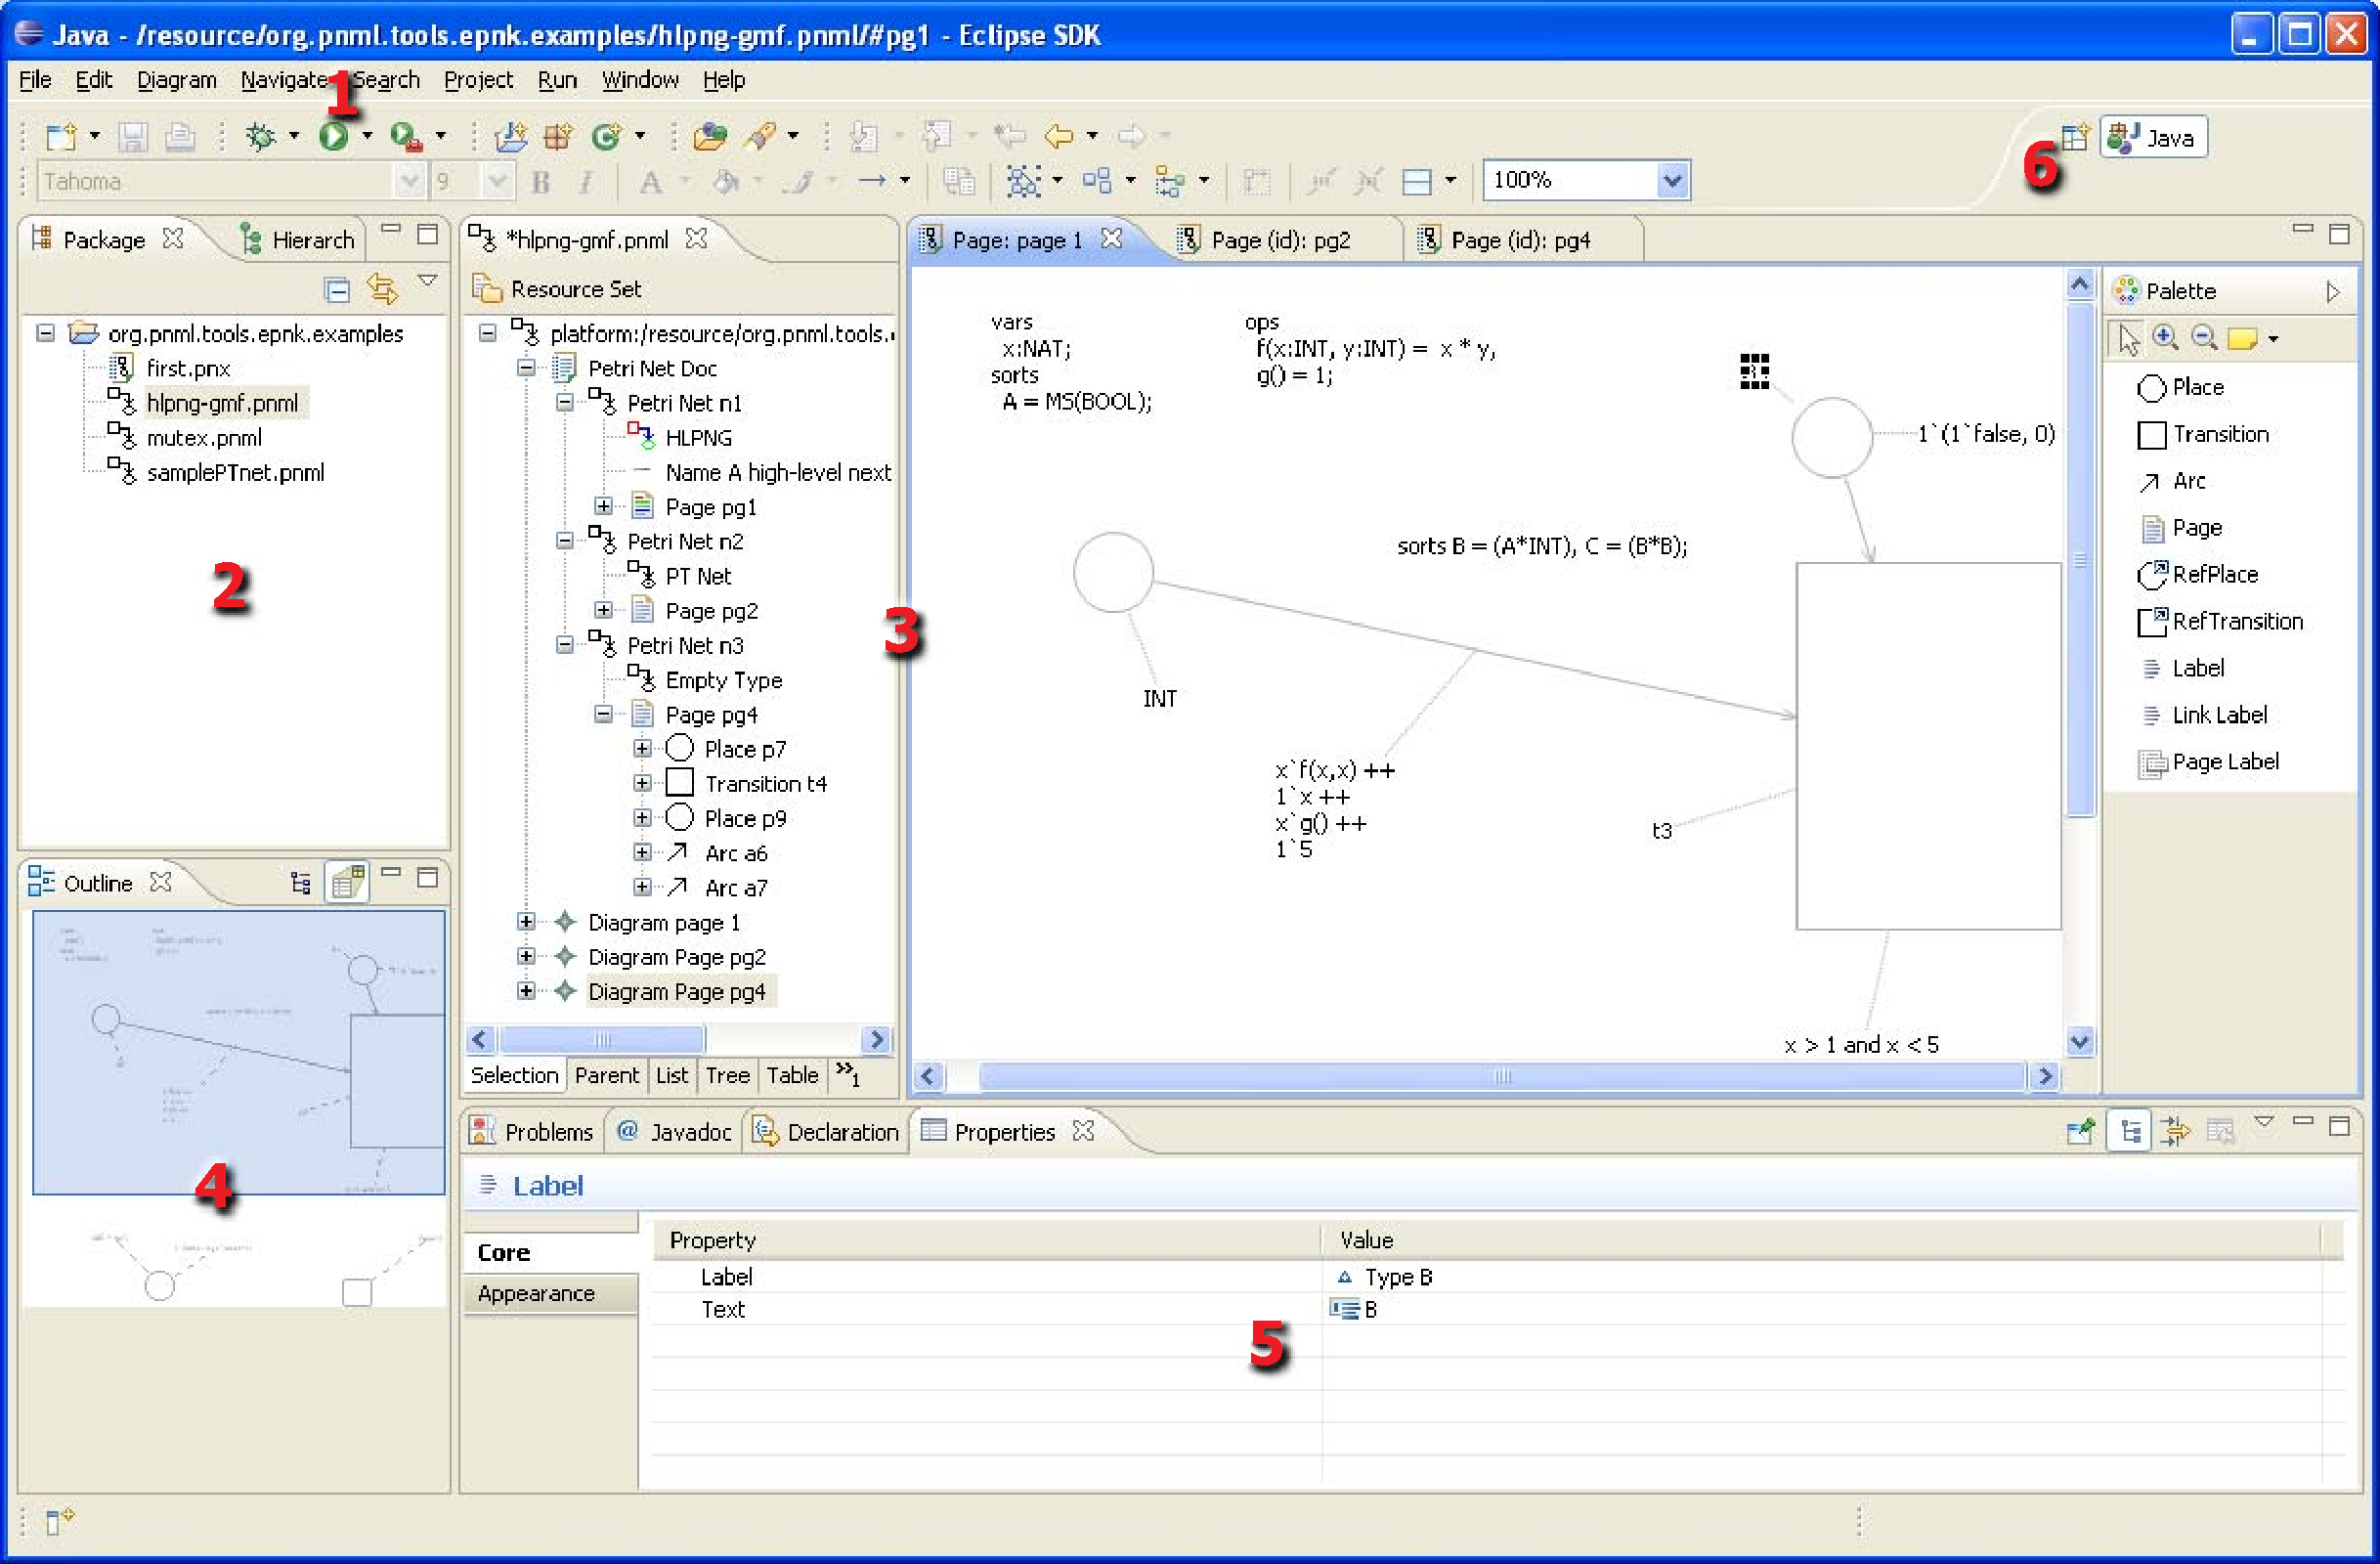
\includegraphics[scale=.30]{IDE-marked}}
  \caption{The Eclipse workbench}
  \label{fig:workbench}
  \index{Eclipse!Workbench}
\end{figure}

On the left-hands side, marked by (2), you can see the \emph{package explorer},%
  \index{Eclipse!Package explorer|DEF}
which gives you access to all the files in your workbench. The package explorer
can be used for browsing through the existing files and for manipulating,
renaming, copying, moving, and deleting them. This is very much like the file
explorer of your operating system. Eclipse actually has different kinds of explorers,
depending on the perspective and the user's preferences. The package explorer is
made for Java development projects. For our purposes, any of these explorers
would do, like for example the ``navigator'' or the simple ``project explorer''.
To find and open one of these other explorers, you can use the menu ``Show View'' in the
menu bar menu ``Window''. All these explorers have some important concept
in common, which concerns the organisation of files in the workbench: the
top-level ``folders'' are actually not folders, but they are \emph{projects}.
This is relevant only when creating these projects. You can create a folder
or file in the workbench only after you have created some project; this can be
done via the ``File'' menu or by a right-click in the explorer and then
selecting ``New''$\rightarrow$``Project''. Note that in the dialog, you can
create many different kinds of projects; for us the kind ``Project'' in
category ``General'' will do. Then, files can be created within
this project. 

In the center (3), you can see the \emph{editor area} of Eclipse. This is%
  \index{Eclipse!Editor|DEF}
where all the editors that are started in Eclipse will be opened. Note that
there can be many editors open at the same time (in our example, there are four
editors open). Typically, you can see only one at a time and the others are
hidden below it. But, you can move the editor tab to some border of the editor
area, so that you can see the contents
of two or more editors at the same time. In our example, there is
a tree editor of a complete Petri net document open on the left-hand
side, and, on the right-hand side, you can see one specific page open
in a graphical editor (the graphical editors for some other pages are hidden
beneath). Note that, even though there can be many editors open and even visible
at the same time, there will always be only one editor that is active. This
editor and what is selected in it determines what you see in some other
views. For example, you can see the \emph{outline view} (4)%
  \index{Eclipse!Outline view}
of the page or you can see the
property of the currently selected element in the \emph{properties view} (5)%
  \index{Eclipse!Properties view}
at the bottom.  In order to open an editor on some resource in the explorer,
you would, typically, double click on the resource you want to open. This will open
the \emph{default editor}%
  \index{Eclipse!Default editor|DEF}
on the selected resource. You can also use the right mouse button on a resource
to open a pop-up menu and then select ``Open with'' 
to select a specific editor for this purpose. The way of editing the contents
of a resource depends on the kind of editor; generally, it is straightforward.
Saving the file can typically done by a shortcut (like CNTRL-S) in all 
editors (or via the ``File'' menu in the menu bar).
An editor can be terminated (closed) either by clicking the close
symbol on the tab of the editor or via the ``File'' menu in the menu bar.

Most editors support undo and redo of the latest changes, which you can
access via the ``Edit" menu or via the CNTRL-Z and CNTRL-Y shortcuts.

Note that the graphical editor of the ePNK cannot be initiated directly from
the explorer since the resource could have many pages and a page is
not the top-level element. When you open a PNML file, a tree editor
will be opened that shows the structure of the Petri net. The graphical
editors for a page of a Petri net can be opened by a pop-up menu (right
mouse button) on pages in the tree editor for Petri nets or by a double
click on the page (see Sect.~\ref{sec:graphical-editor} for details).

All the other areas of the workbench are% 
  \index{Eclipse!View|DEF}
\emph{views}\footnote
{Actually, also the resource browsers are views.}%
. In Eclipse, views are used for many different purposes. The
views that are most relevant for us, are the \emph{outline}%
  \index{Eclipse!Outline view|DEF}
(4), the \emph{properties}%
  \index{Eclipse!Properties view|DEF}
(5), and the \emph{problems view}% 
  \index{Eclipse!Problems view|DEF}
(not visible in
Fig.~\ref{fig:workbench}). The outline gives an overview of the contents of
the currently active editor and, in case of a graphical editor, allows us to
quickly move around the visible area of this editor. The properties view
shows some details of the currently selected element in the editor; in many
cases, the properties view also allows us to edit some properties. Note that,
initially, the properties view might not be open. You can, typically, open it
from the active editor via a context menu on the right mouse button:
In the pop-up menu that opens, there will be a menu ``Show Properties
View'', which opens the properties view. You can also open
the properties view via 
``Window''$\rightarrow$``Show View''$\rightarrow$``Others ...'' and
then selecting ``Properties'' in the category ``General''.

We mentioned already that the Eclipse workbench can appear
in different ways, which is defined by the chosen \emph{perspective}%
  \index{Eclipse!Perspective|DEF}
(and some user-specific settings). The perspective can be changed via
the tools at the top-right of the workbench, which are marked with (6)
in our example. We do not need to change it; but if, for whatever reason, you
end up in a wrong perspective, by clicking on the left symbol,
you can open the ``Open Perspective'' dialog. There, you can
select the perspective ``Resource'' or, if you like, ``Java'' (which is
the default perspective).
 
If you are interested in more details in the Eclipse workbench,
you can have a look into the Eclipse help
(``Help''$\rightarrow$``Help Contents'') or at one of the
many books or online articles;
\url{http://www.vogella.de/articles/Eclipse/article.html} could
be a start.%
  \index{Eclipse|)}%
  \index{Eclipse!IDE|)}

\section{Creating Petri net files}
\label{sec:CreatingPetriNetDocuments}

This section explains how to create new ePNK files. Note that there
are two formats in which the ePNK can save a Petri net. The first and
recommended format is PNML. The second format is the XMI-serialisation of the
PNML models, which we call PNX.  Note that PNX, is part of the ePNK since XMI is the
standard serialisation mechanism of the EMF technology used for implementing
the ePNK and, therefore, came for free. Whether PNX really should be a part of
the ePNK distribution is yet to be seen. Therefore, the focus of
this users' guide is on PNML.

The easiest way of getting started with the ePNK is obtaining existing PNML
files from somewhere else and just copy them to the workbench. For example, you
could get some examples from the ePNK home page: 
\url{http://www2.compute.dtu.dk/~ekki/projects/ePNK/}. You can also use a text
editor and create a simple text file with file extensions ``.pnml'' and insert
the single line
\begin{lstlisting}[language={[structured]PNML},keywordstyle=\underbar]
  <pnml xmlns="http://www.pnml.org/version-2009/grammar/pnml"/>
\end{lstlisting}
to this file, which is an empty Petri net document without any nets in it.

The ePNK also provides you with a wizard for creating a PNML document.
Like all Eclipse creation wizards, this wizard is started via the ``New''
menu, which can be either accessed by the ``File'' menu from the menu bar or via
the pop-up menu that opens on a click to the a right mouse button in the
explorer.
Then, select ``Other...'' (the short-cut to that would be pressing
CNTRL-N in the explorer) and in the newly opened ``Select a wizard''
dialog choose ``PNML Document''%
  \index{PNML Document|DEF}
from the ``ePNK'' category and press
``Next''. In the next dialog, you must choose a name and, if you
want, you can choose a different folder in which this file should
be created. Pressing ``Finish'' will create the file; then, the
newly created file will be opened in a tree editor (see
Sect.~\ref{sec:tree-editor});%
  \index{ePNK!Tree editor}
note that you also can continue the
creation process by pressing ``Next'', which will allow you to chose an
XML-Encoding.  Note that, in the dialog with the encoding, there
is also a field asking for the ``Model Object''; but you cannot
choose anything here since PNML, in contrast to other formats,
has a fixed root object that cannot be changed: ``PetriNetDoc''. 

Note that in the same wizard category ``ePNK'' there is another
wizard called ``PNX Document''.%
  \index{PNX Document|DEF}
When you use this wizard, a PNX file
will be created. In this wizard, you can select a root element different
from the PetriNetDoc -- but this would be reasonable only in very special cases
(and when you know exactly what you are doing).
 
\section{The tree editor}
\label{sec:tree-editor}

\index{ePNK!Tree editor|(DEF}
As mentioned earlier, the ePNK provides two kinds of editors
for Petri nets: the \emph{tree editor}, which allows us to create,
modify, and delete all parts of the Petri net in a tree-like
structure; and the \emph{graphical editor}%
  \index{ePNK!Graphical editor}
in which a page
of a Petri net with its places, transitions, and arcs can
be edited in a graphical way. Clearly, the graphical editor
is more convenient for editing pages than the tree editor.
But, other parts like for example the page structure and the
complete Petri net document are more convenient to edit in the
tree editor. This is why there are two different editors in the ePNK.
The graphical editor for pages is always started from a
selected page -- either in the tree editor or in the graphical
editor. When opening a PNML document from the resource explorer,
it will always be the tree editor that opens. A graphical editor
can be opened by a double click on a page element in an already 
open editor.

\subsection{The tree editor: Overview}
Let us have a closer look at the tree editors first.
Figure~\ref{fig:tree.editors} shows the Eclipse workbench with
two PNML documents open in tree editors. The right one shows the tree editor
opened with the PNML file (``test.pnml'') with the single line as discussed in
Sect.~\ref{sec:CreatingPetriNetDocuments}. Therefore, it contains only the
Petri net document element without any contents. The other PNML document, which
is open on the left-hand side (``hlpng-gmf.pnml''), shows a Petri net document
with three nets that have different types.
 
\begin{figure}[hbt!!]
  \centerline{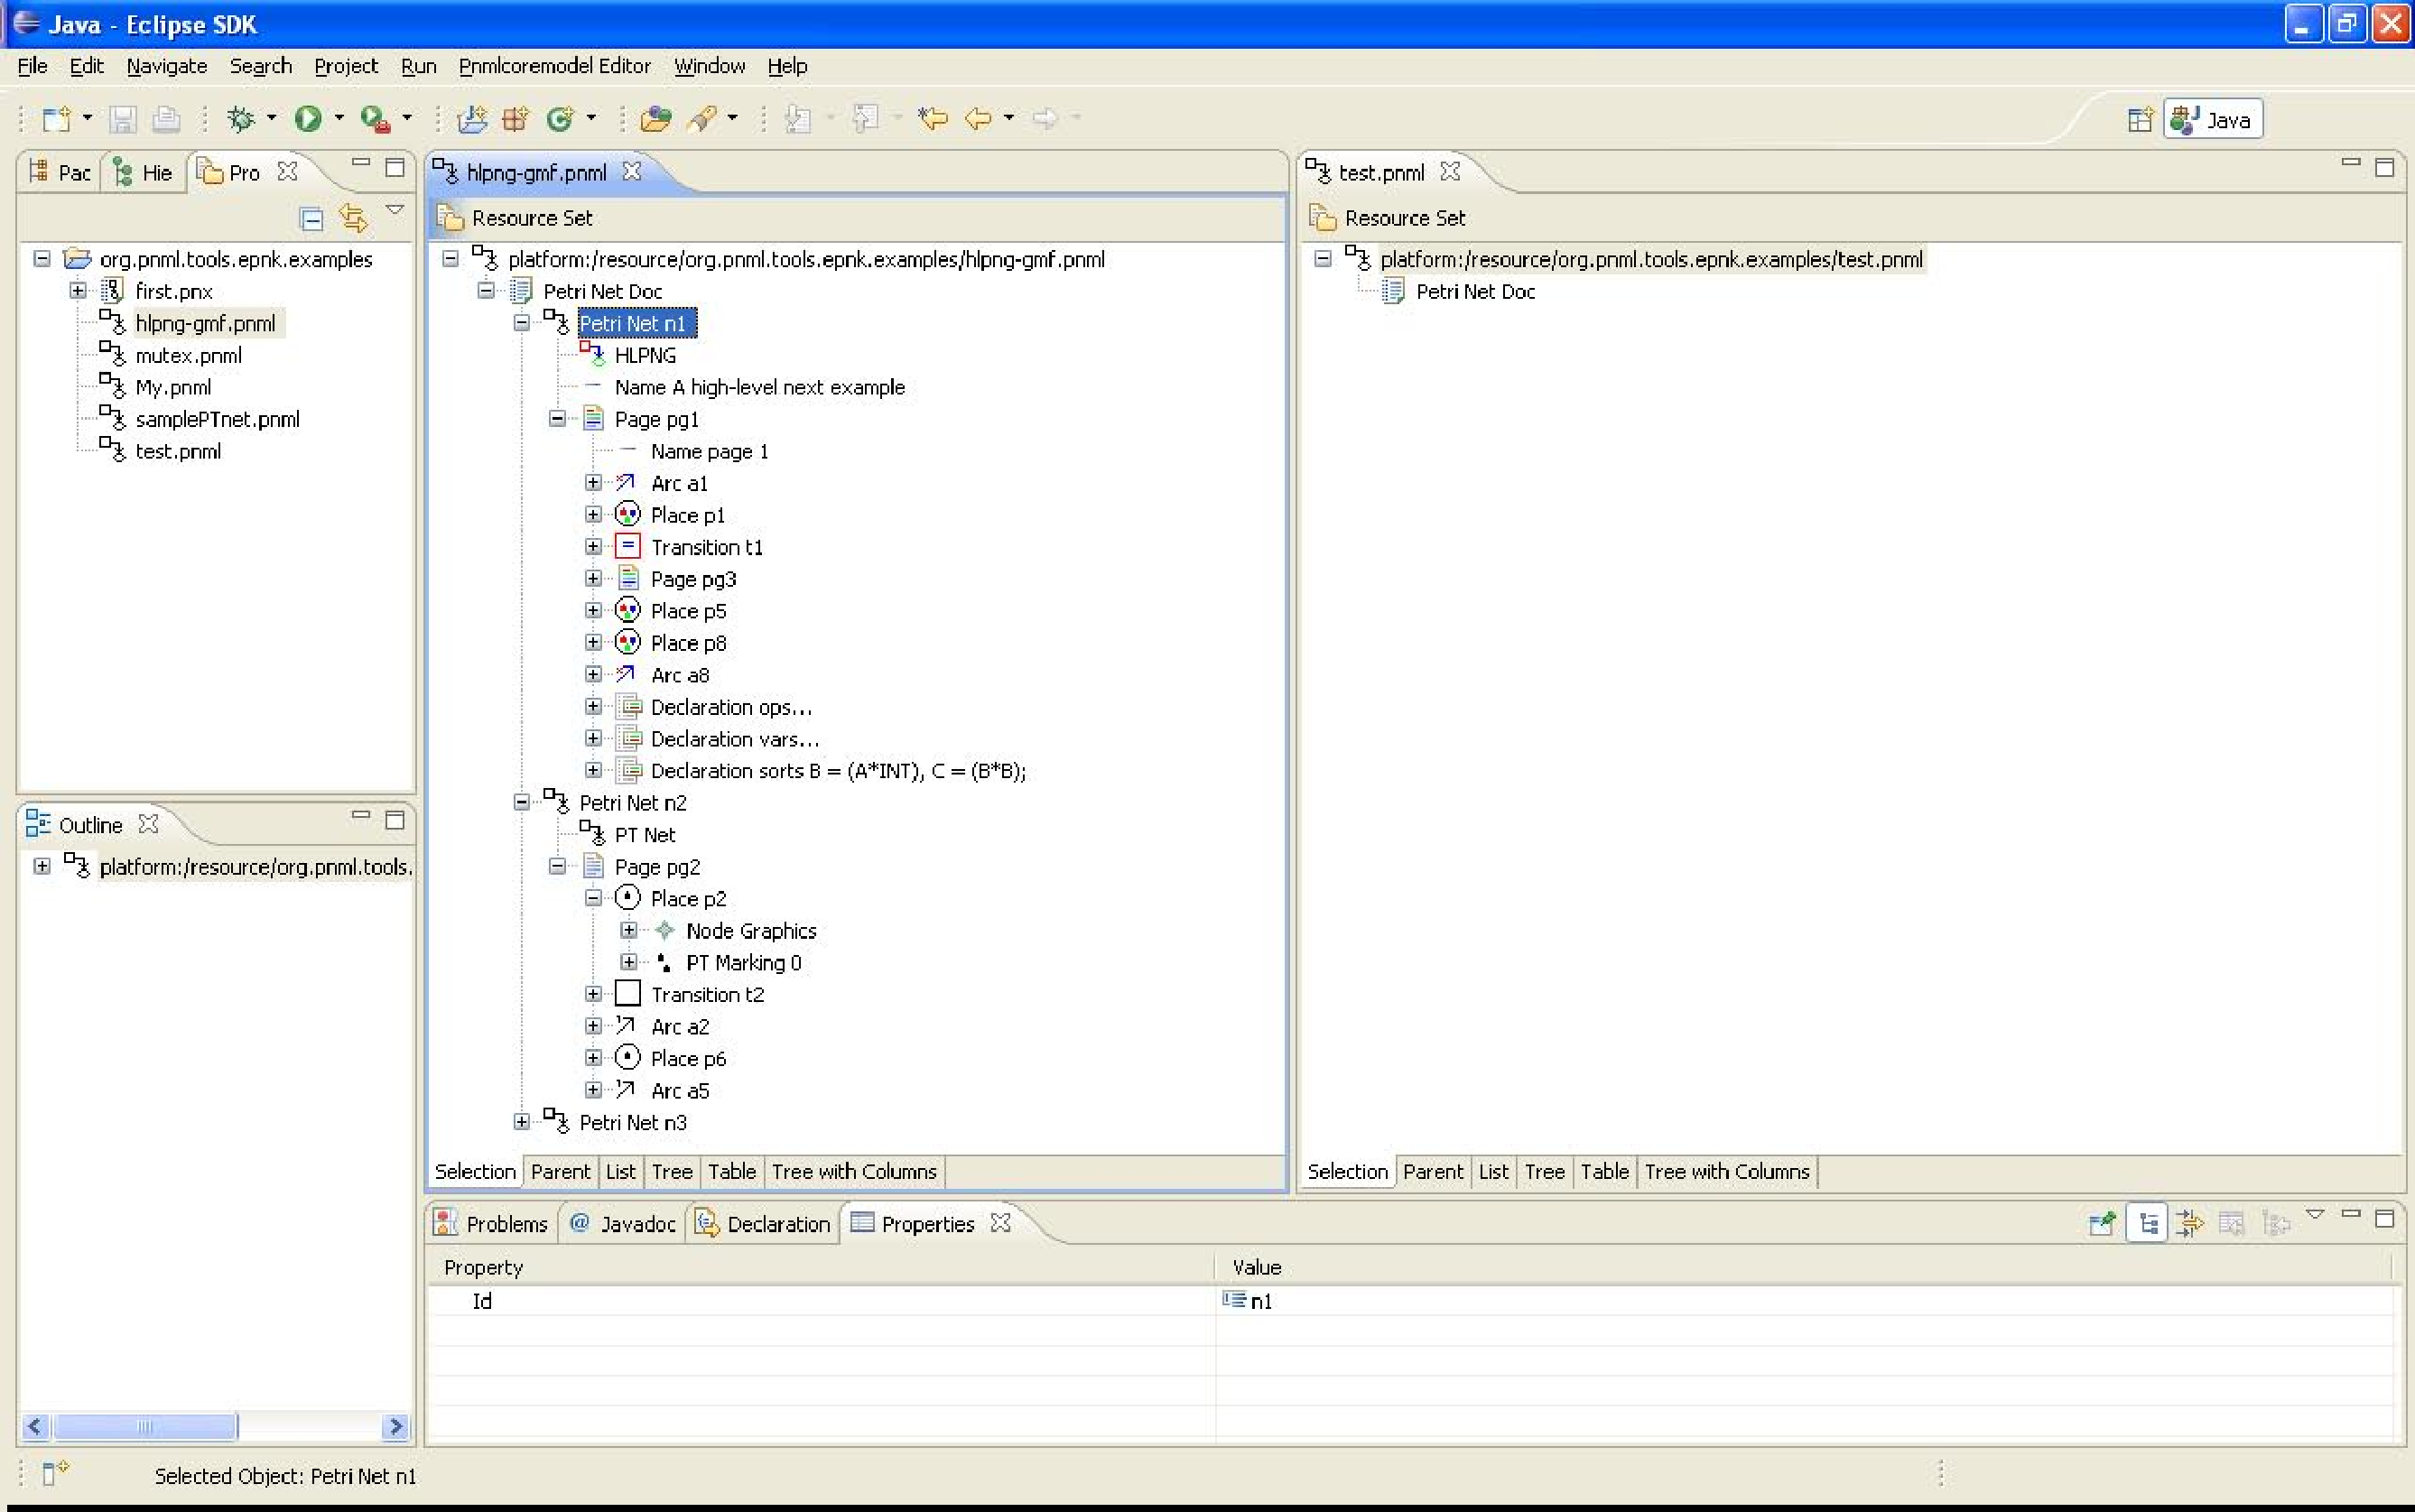
\includegraphics[scale=.28]{TreeEditors}}
  \caption{Two Petri net documents in tree editors}
  \label{fig:tree.editors}
\end{figure}

These documents were opened from the explorer by a double click\footnote
 {Remember, that you can use the pop-up menu to make an explicit choice
  by which editor you want to open the file. This way, you can open
  the file with a text editor, so that you can see the PNML
  it produces. On a double click, the file is opened
  with the editor you had selected the last time.}
on the respective file in the workbench's explorer. Let us briefly go through
what you see in the Petri net document ``hlpng-gmf.pnml''.  The top-line shows the
actual \emph{resource}%
  \index{Eclipse!Resouce|DEF}
or file in which this document is stored; the second
line is the symbol for the Petri net document itself -- all documents will
follow this structure in the tree editor. Then you can see that
there are three Petri nets contained in this document (with \emph{ids}%
  \index{ePNK!id}
n1, n2, and n3); the last net is actually not folded out because
its was not fitting to the screen. The first line below the 
Petri net is the type of the Petri net. The first net
is a high-level net, which is named \emph{HLPNG}%
  \index{HLPNG}
according to ISO/IEC~15909-2;
the second net is a Place/Transition-System, called PTNet according
to the standard. You can also see that the nets contain places, transitions,
and arcs, which are indicated by corresponding icons. You can also see
some pages and sub-pages.  Note that the icons for the places, transitions,
and arcs are different for the two different Petri net types, so that it
easier to distinguish them on a first glance. In the properties view at the
bottom, you can see the properties of the currently selected element, which is
Petri net n1; the only property is its id. Note that this net has a
name; this, however, is not shown as a property, but as a \emph{child element}%
  \index{Eclipse!Child element|DEF}
of the net, which is true for all labels of Petri nets. In this case, the name is 
``A high-level next example''.

\subsection{Creating elements}
\label{subsec:creating-elements}

You can unfold all the sub nodes (children) of the net and this way
inspect the complete document in all details. More importantly, however,
you can create the basic elements of the Petri net document. You can
create new nets (along with their type) and their pages. And from there, you
would use the graphical editor to draw the rest.  This basically works by
inserting \emph{child elements}.%
  \index{Eclipse!Child element|DEF}
Inserting a child element is done by
right-clicking on the element to which you want to add a child, then selecting
``New Child'' in the dialog that pops up, and then selecting the appropriate
element. Figure~\ref{fig:new-child-element} shows the pop-up dialog when
inserting a new Petri net to the Petri net document.

\begin{figure}[hbt!!]
  \centerline{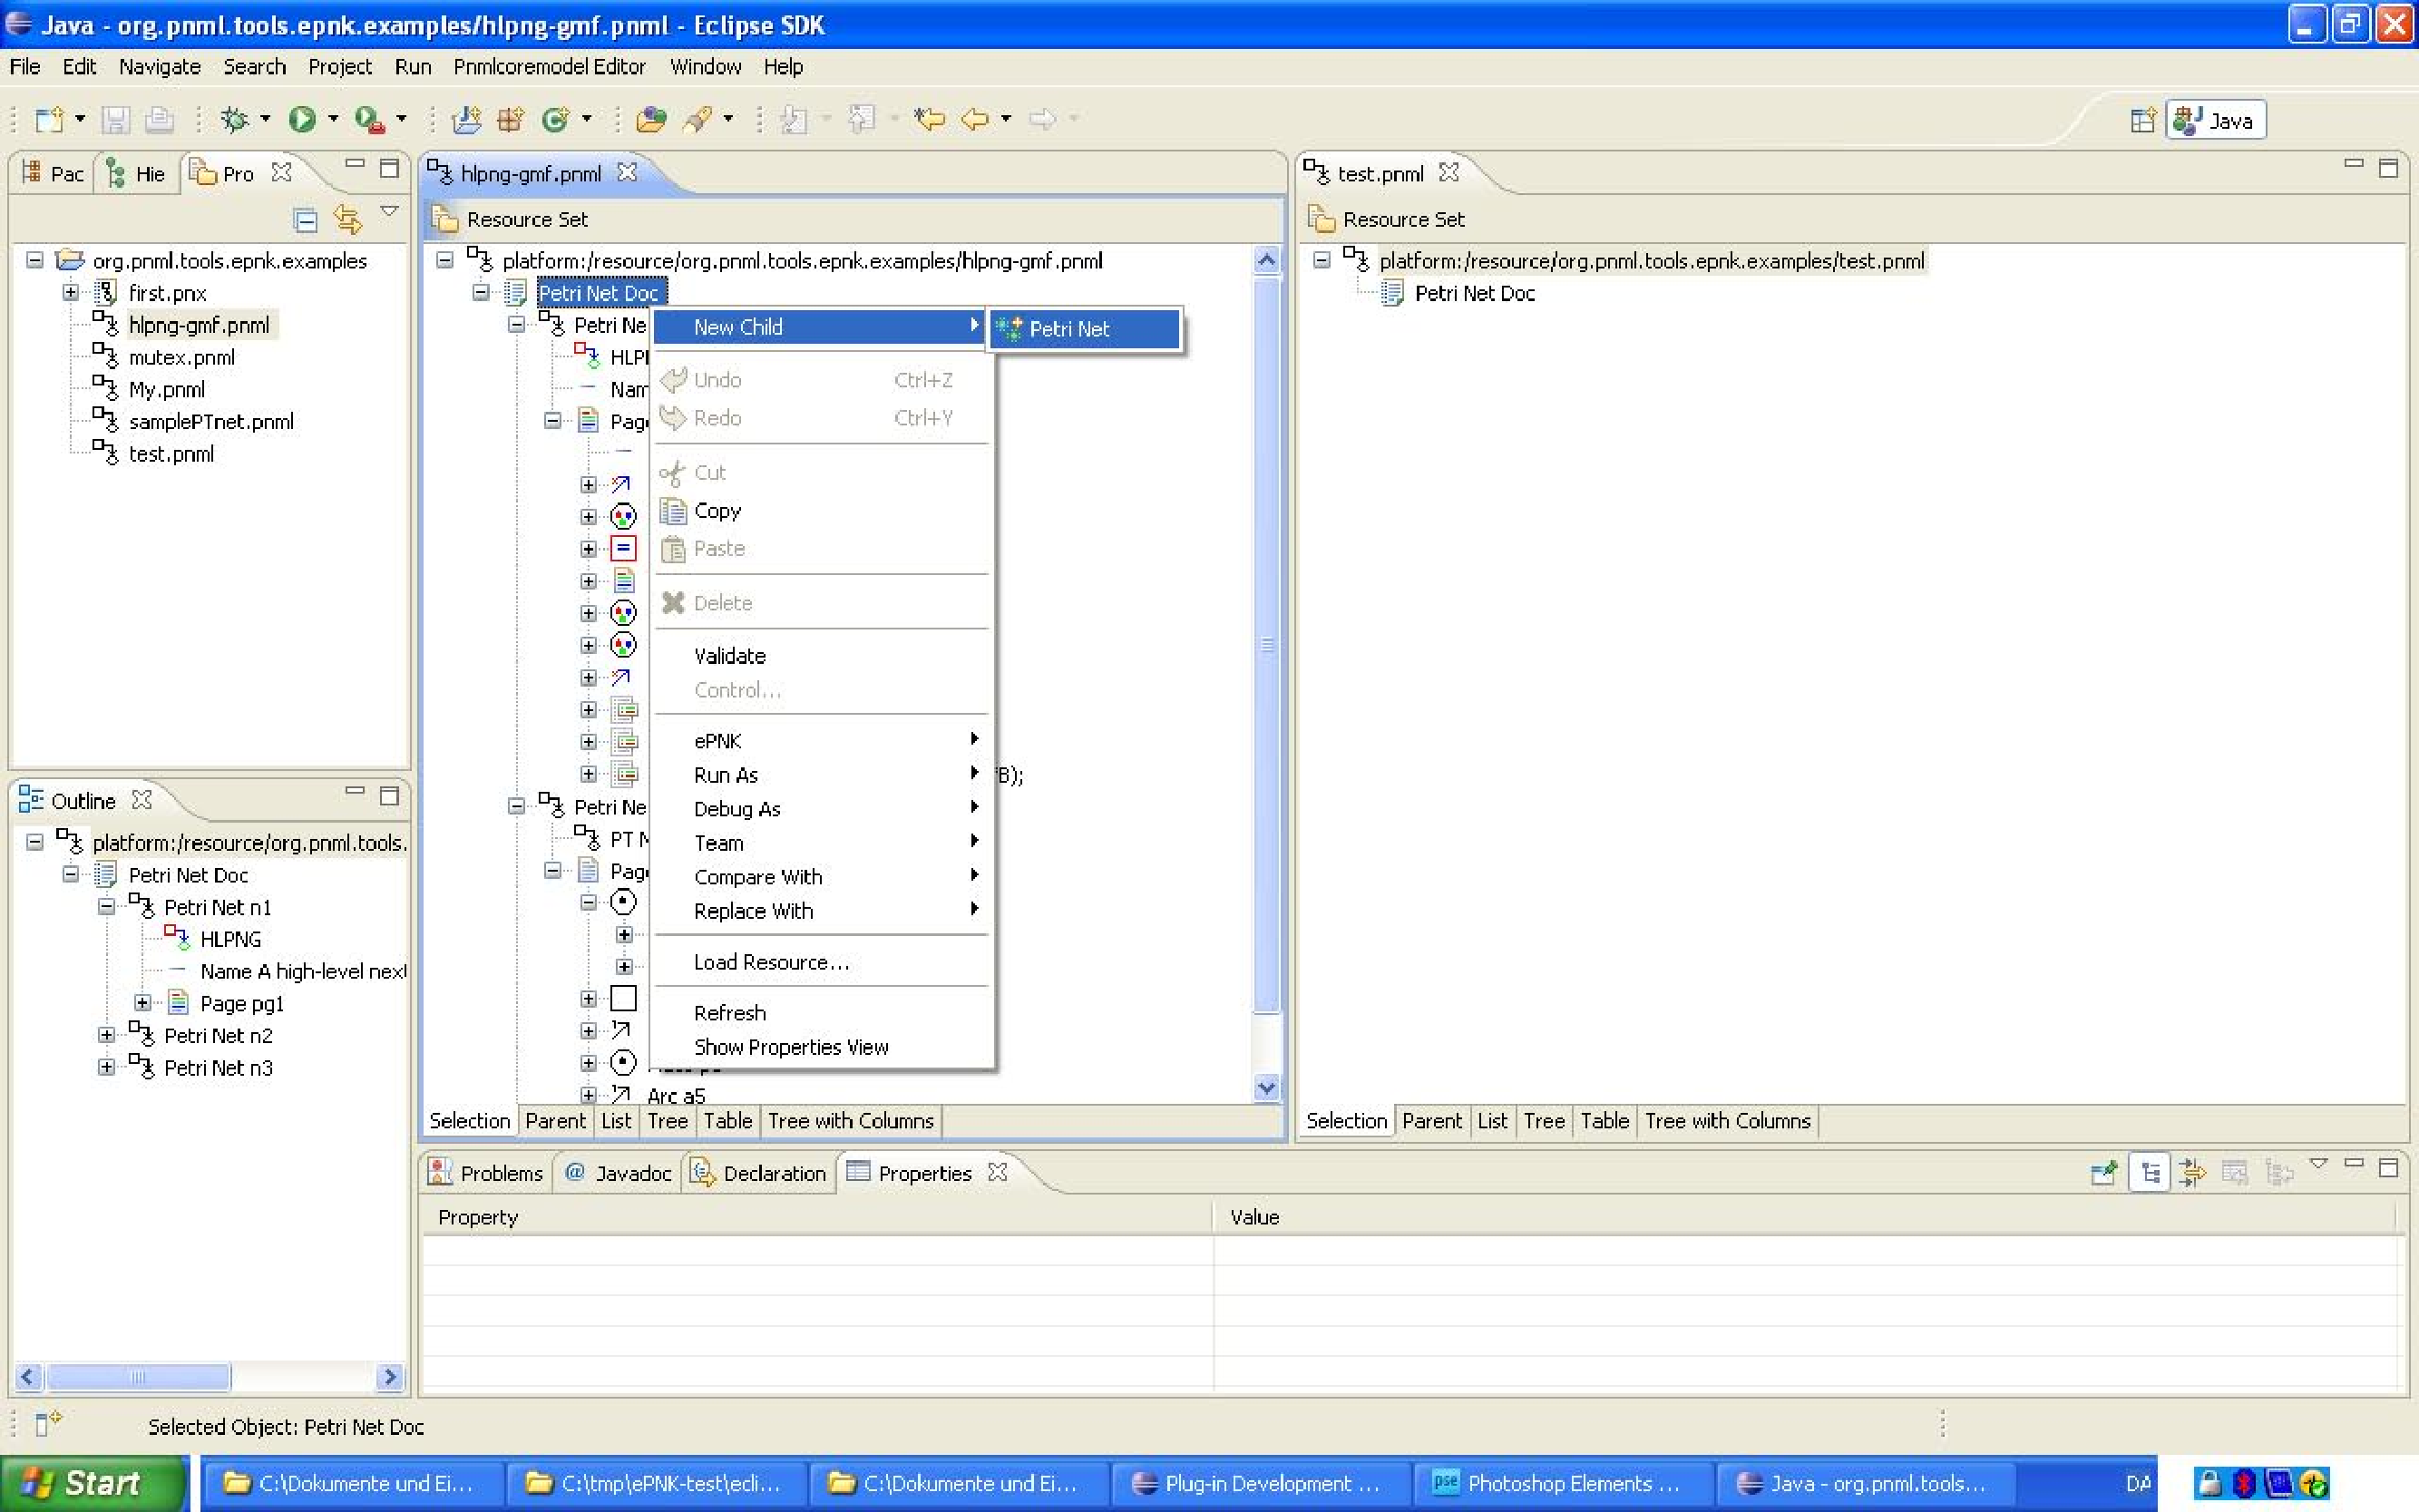
\includegraphics[scale=.28]{NewChildElement}}
  \caption{Pop-up menu when inserting a new Petri net}
  \label{fig:new-child-element}
\end{figure}

Note that this dialog will show all available Petri net types, from which
you will need to select. Then a new net of that type will be created. Note
that the created net will contain a child element, which represents
the type of this net. You should never delete or change this net type
manually\footnote
  {Unless you know exactly what you are doing.}.
You will find some more information on the Petri net types that
are deployed together with the ePNK in Sect.~\ref{sec:petrinettypes}. 

After you have created a new Petri net, the name of the net and new
pages can be inserted to it by via the ``New Child'' pop-up menu on the
selected Petri net similar to creating the net -- just select the
kind of element you want to create.

\subsection{Saving the document}
\label{subsec:save-documents}

As discussed in Sect.~\ref{sec:Eclipse-IDE}, you can save the net via the
``File'' menu or with the CNTRL-S shortcut. Note that saving the net
must be done -- and can be done only -- in the tree editor. Therefore,
only the tree editor shows the dirty-flag, when the editor contains
unsaved changes.

\subsection{Validating and correcting the document}
\label{subsec:validation}
\index{ePNK!Validation|(DEF}

Before saving a PNML document, it is a good idea to \emph{validate} the
net. This will check whether all the constraints that PNML and the
respective Petri net types imposes on the Petri net document are met. It is
possible to save a document that does not properly validate, and you would
be able to load the file again. But, if you save a file that
does not properly validate, you cannot be sure that the saved document
is ISO/IEC~15909-2 conformant PNML, and other tools might not be able to load
it.

There are many things that can be wrong and need validation
on a Petri net document. Most of them are type specific (such as the requirement
that an arc must run from places to transitions or the other way round only);
these Petri net type specific constraints will be discussed in
Sect.~\ref{sec:petrinettypes}. But, there are also some general constraints:
\begin{itemize}
  \item Every Petri net object must have an id and this id must be
        unique in the scope of this document.
        
  \item Arcs may only connect nodes which are on the same page (as
        long as you are using the graphical editor, this constraint
        cannot be violated; but if you do changes in the tree editor,
        this could be violated).
        
  \item There must not be cycles on the references between reference
        nodes, and all reference nodes must refer to a node.
        
  \item A reference node must refer to a node within
        the same net.  
\end{itemize}

In order to identify which constraints are violated, you can use the
validation feature. Click on the right mouse button on the Petri net
document; then, in the pop-up menu, select ``Validate''. The result
of the validation will be shown in a dialog; the results of the validation
is also visible in the \emph{problems view}\footnote
  {If the problems view is not open, you can open it by
   ``Window''$\rightarrow$``Show View'' $\rightarrow$``Problems''.}%
  \index{Eclipse!Problems view}
after the validation as shown in Fig.~\ref{fig:validation}. Most of these
errors are actually coming from high-level nets. But, there is also a general
constraint violated in this example: some IDs collide (line 5 and 6 in the
problems view), which means that the same ID is used twice in this document.

Note that you can double-click on the individual problems in the problems
view. Then, an editor is opened with the element to which this problem refers to
selected. If there is a graphical editor open for the page that contains 
the element with the error, the ePNK will show the selected element in the
graphical editor; if there is not graphical editor open with that element,
the element will be shown in the tree editor. 

\begin{figure}[hbt!!]
  \centerline{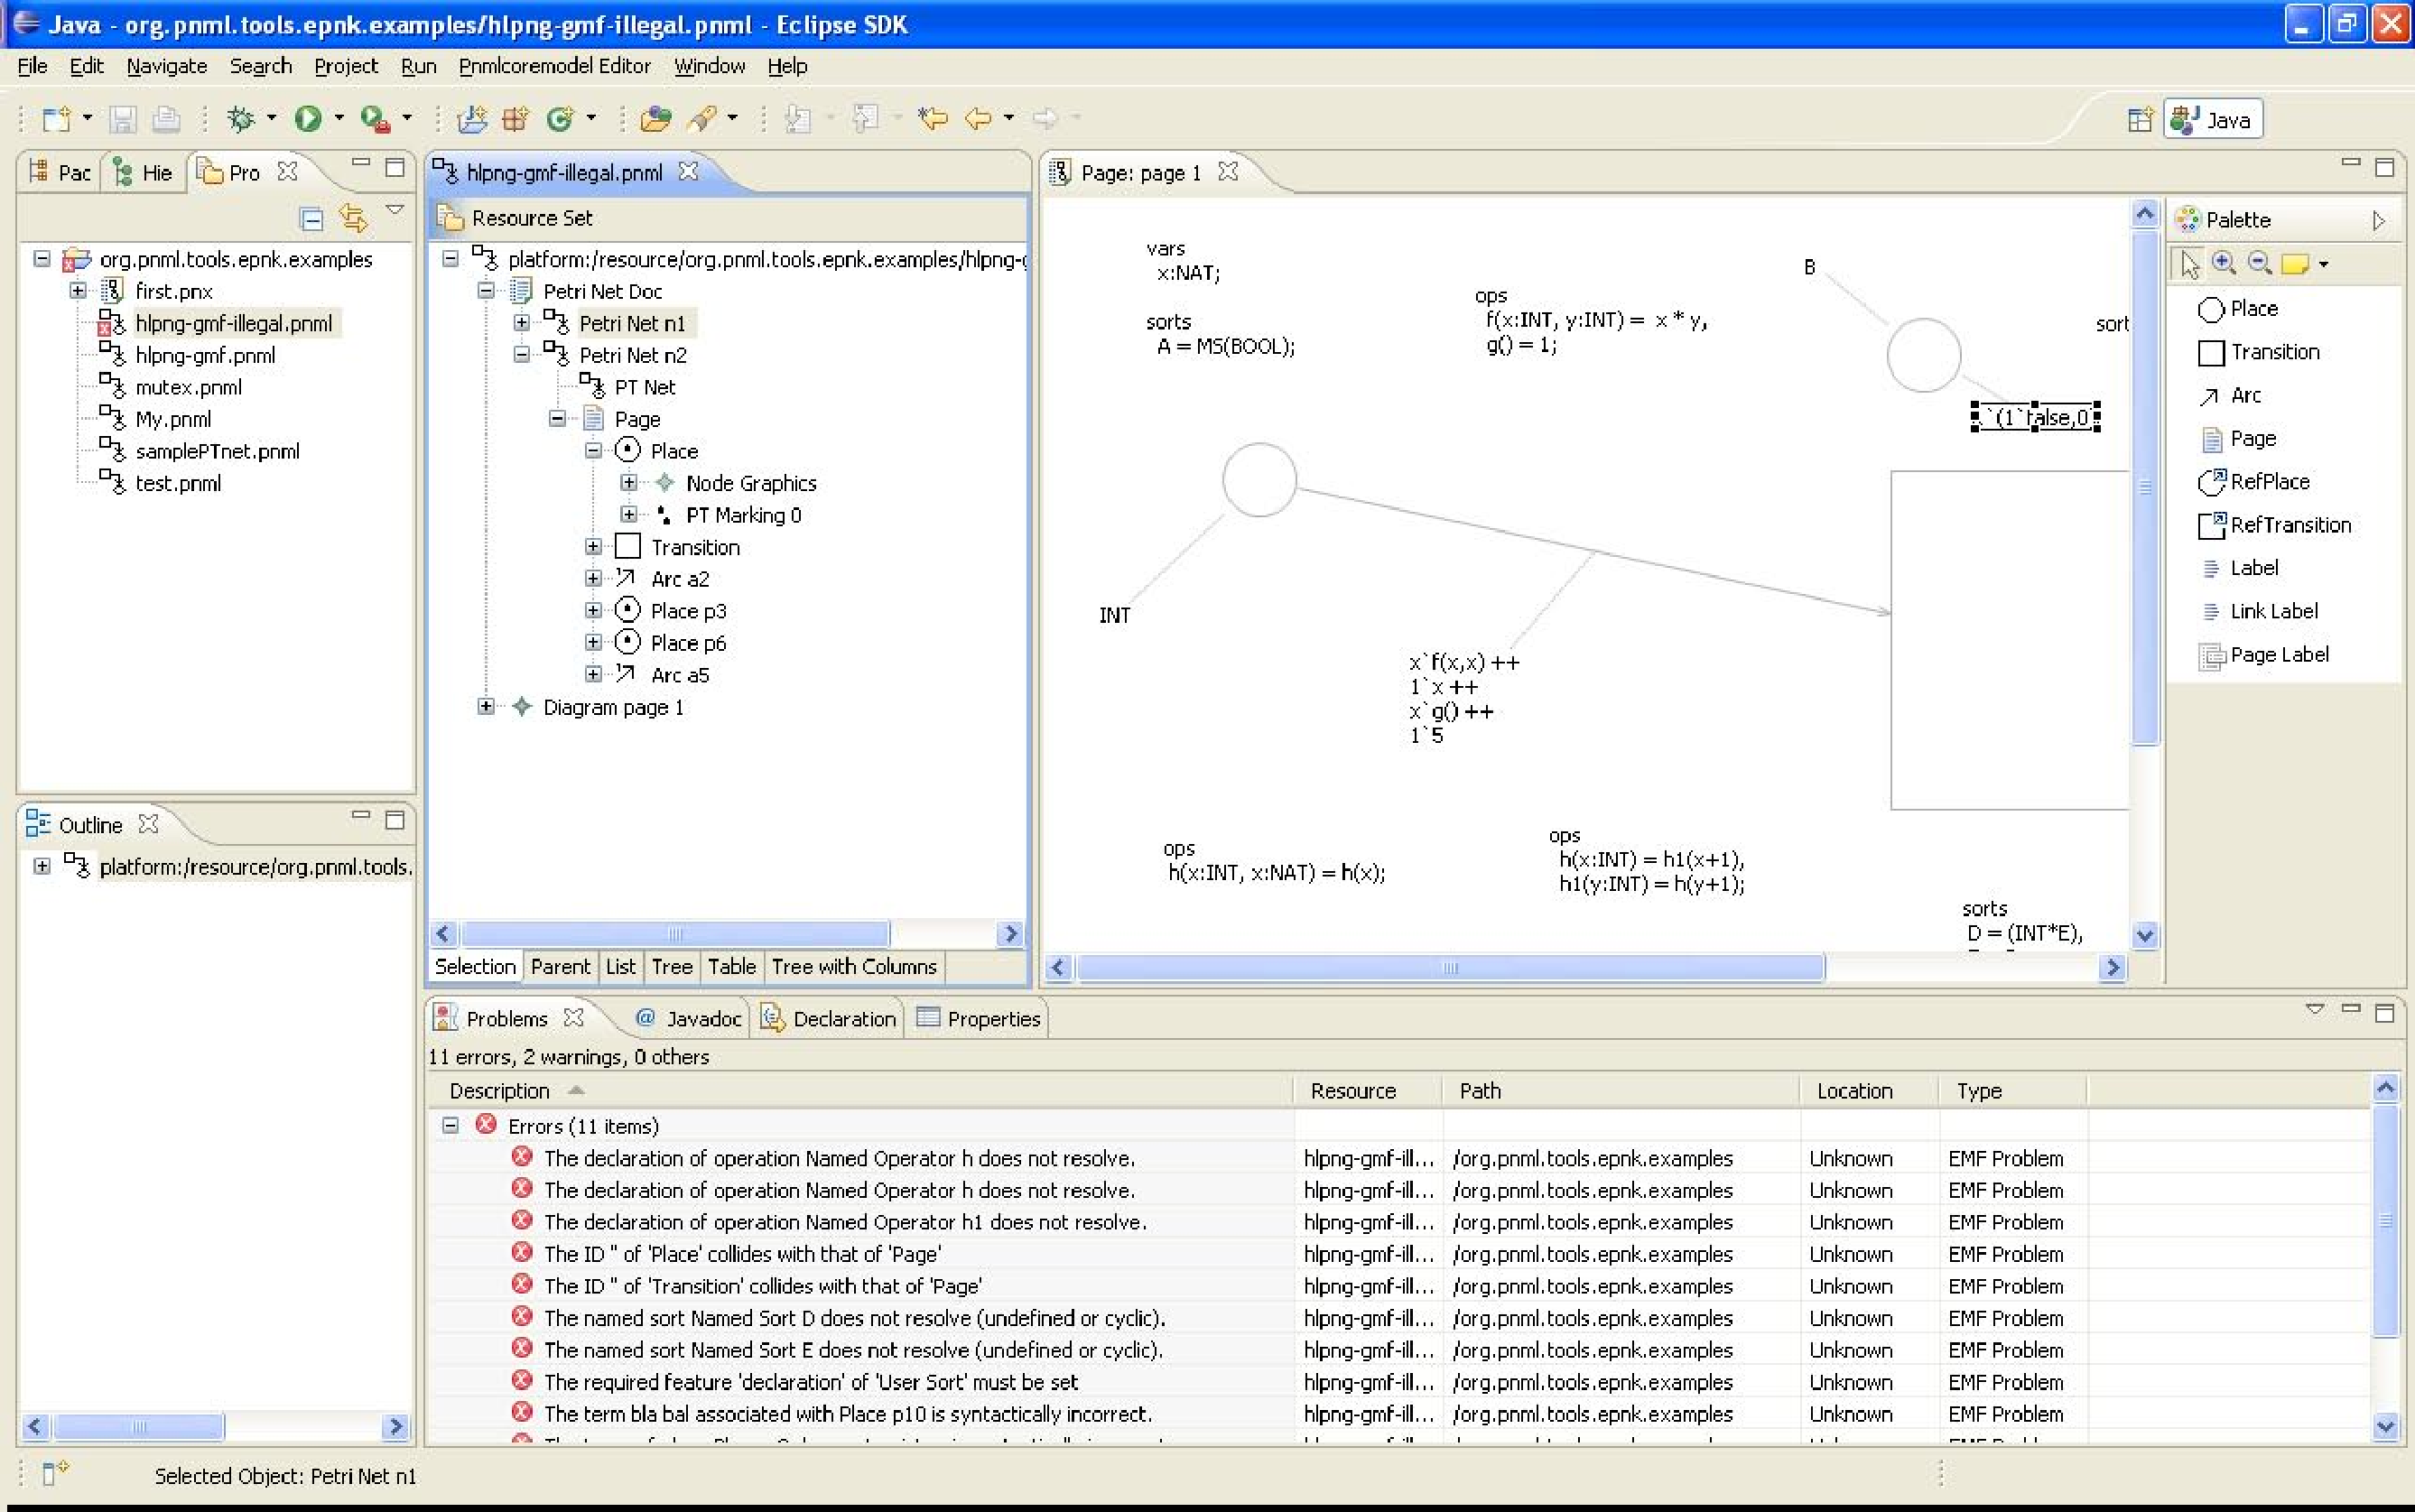
\includegraphics[scale=.25]{Validation}}
  \caption{The problems view with many constraint violations}
  \label{fig:validation}
  \index{Eclipse!Problems view}
\end{figure}

In order to reduce the number of errors, you can also do a validation
on sub-elements of the Petri net document, which could be a net
or even a single page. Ultimately, however, you must validate
the complete Petri net document.

In our example, there are some problems that
can be fixed automatically. For example, ids can be set automatically.
The ePNK provides an action for this. To this end, select the Petri net
document, click the right mouse-button, and then select
``ePNK''$\rightarrow$``Add missing IDs'' in the%
  \index{ePNK!id|DEF}
pop-up menu. This will fix all problems with the ids within a
Petri net document. Actually, there is a shortcut: a double-click
on the Petri net document element in the tree editor will automatically add all
the missing ids.

Some other errors might need some manual changes, which could typically
be made in the graphical editor of pages.

\subsection{Other Petri net information}

In principle, you can inspect and edit all the information of a Petri net
document in the tree editor. In our example from
Fig.~\ref{fig:new-child-element}, you can also see some labels (declarations
of high-level nets in this case, or a marking of a P/T-System) or
graphical information. If you have a closer look at these examples, you
will also find some other types of elements such as tool specific information --
and once graphical editors are started some auxiliary data.  But, it is
strongly recommended not to change any of this information in the tree
editor\footnote
 {Once the features of the ePNK that are really needed in the editor are fixed,
  the parts that should not be edited in the tree editor will probably be
  removed or at least made read only.}%
.%  
  \index{ePNK!Tree editor|)}
  \index{ePNK!Validation|)}

\section{The graphical editor} 
\label{sec:graphical-editor}

\index{ePNK!Graphical editor|(DEF}

For editing the contents of pages, the graphical editor should be used. The
graphical editor can be opened by right-clicking on the respective page in the
tre -editor and then, in the pop-up menu, selecting ``ePNK''$\rightarrow$``Start
GMF Editor on Page''. A shortcut for this is double-clicking on the page.

When you open a graphical editor on a page for the first time, you will
be warned that this change cannot be undone -- and no undos will be
possible beyond that point. Therefore, you will be asked whether you
want to proceed with that operation or not. 

Figure~\ref{fig:validation} shows the graphical editor with a page
open in a graphical editor; this is a
page from a high-level Petri net (in this case one with several errors
in it). Normally, this new editor shows on top of the tree editor, but
it can be moved to the right side (click in the tab at the top of the
editor window and move it while keeping the mouse pressed), so that the
tree editor and the graphical editor are visible at the same time.

Figure~\ref{fig:signal-net-attributes} shows another example of a Petri net
opened in the graphical editor, which we will discuss in
Sect.~\ref{subsec:attributes}.

\subsection{Overview of the graphical editor}
\label{subsect:graphical-editor:overview}

On the left-hand side of the graphical editor for the page, you see the
\emph{canvas}%
  \index{ePNK!Canvas|DEF}
with all the Petri net objects on that page represented
in a graphical way.  This includes also the \emph{labels},%
  \index{Label}
which are either attached to an object by a dashed line or attached to the page
itself, in which case it is called a \emph{page label}.%
  \index{Page label|DEF}  

At the top, you see the \emph{tab} of this page, which shows the page's
name (if the page has a name label assigned to it) or its id, or the
path to this page (if the page has neither a name nor an id).   

On the right-hand side, you see the \emph{palette}
or tool bar of the graphical editor. These tools allow you to create
all the Petri net objects.  Note that you can also create sub pages.

There are two different tools for labels. The tool ``Label'' is for creating
labels that are attached to objects, the tool ``Page label'' is for creating
labels that are directly attached to the page that is shown in this editor.

For creating objects and labels, you first select the tool by clicking on
it, and then clicking somewhere into the canvas. For creating an arc, you
select the arc tool and then click on the source object, and keeping the
mouse pressed and move the mouse to the target object. Note that the arc is
not added between two objects, if the Petri net type you are editing
does not allow this.

\subsection{Labels} 
\label{subsec:labels}
\index{Label|(DEF}

When creating a new page label on a page, the graphical editor will show
you all the possible options of legal labels for that type of net Petri net
via a pop-up menu.
Figure~\ref{fig:pagelabel-creation} shows the pop-up menu during the
creation of a page label for a high-level net, where the only option
``Declaration'' is shown here. You can select an option, after which
a label of that kind will be created. You can also abort by either
pressing the ``ESC'' button or clicking somewhere outside the menu.

\begin{figure}[hbt!!]
  \centerline{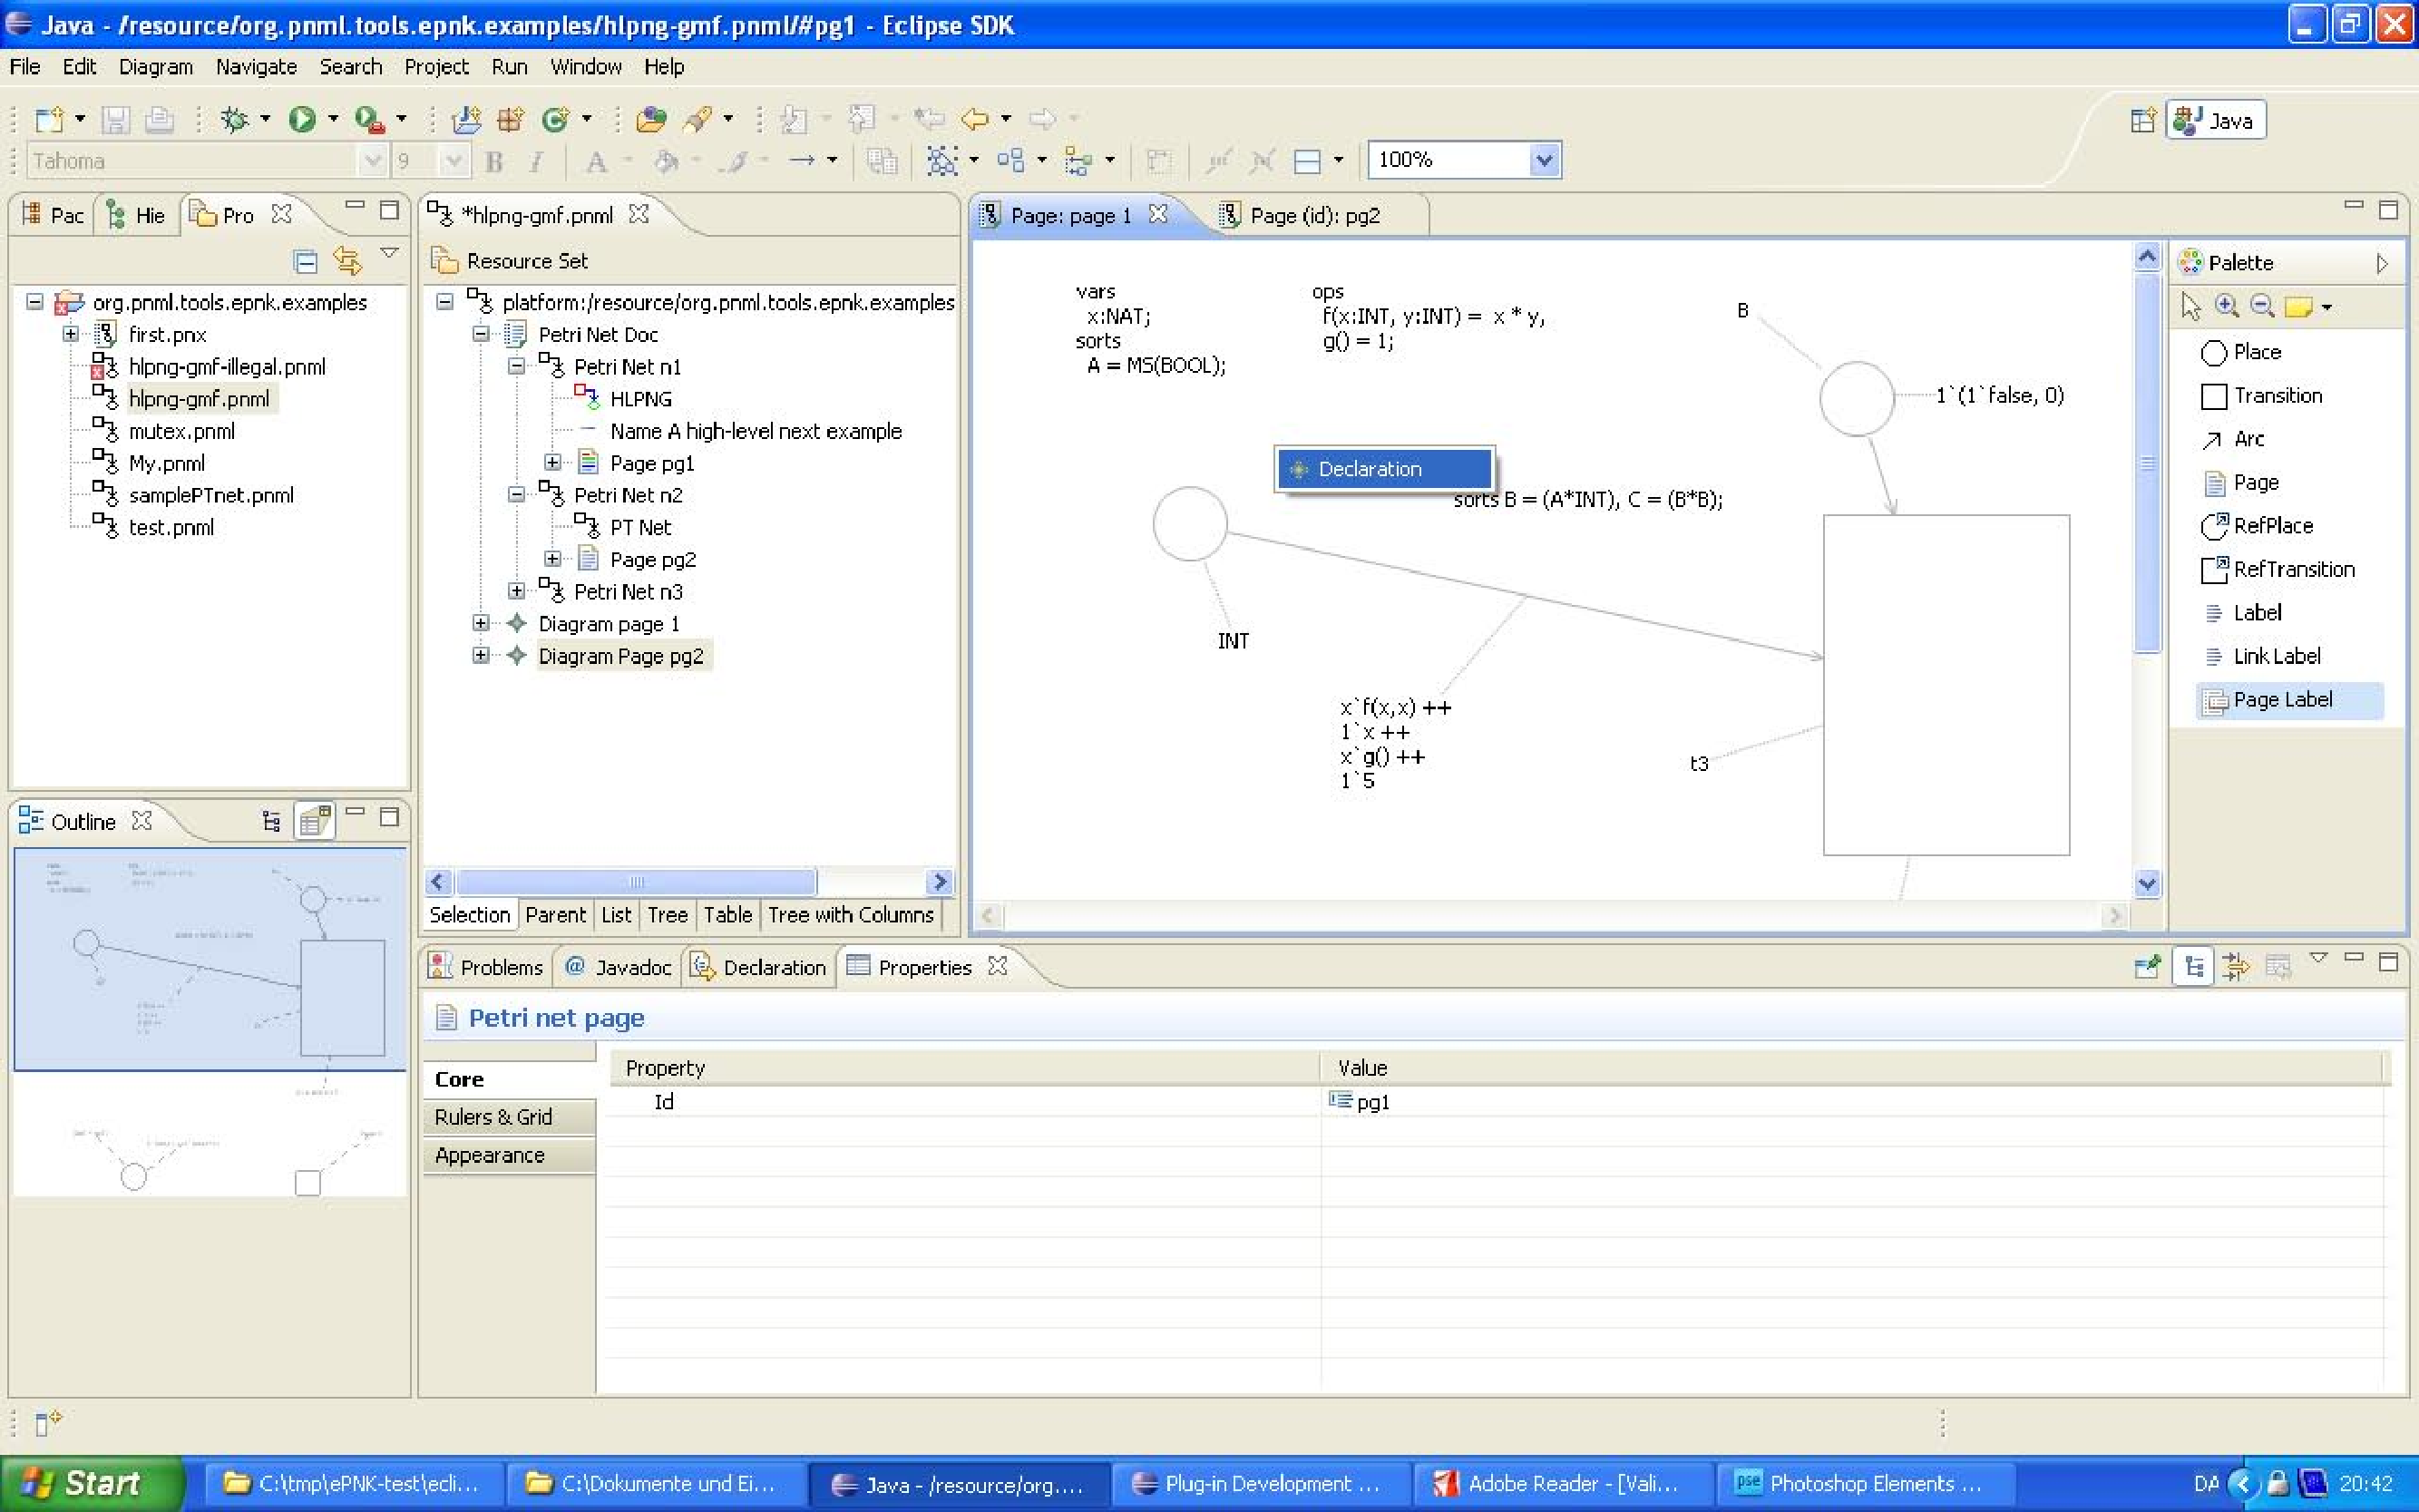
\includegraphics[scale=.25]{CreatePageLabel}}
  \caption{Pop-up menu during page label creation}
  \label{fig:pagelabel-creation}
\end{figure}

The process for creating a label and attaching it to an object is slightly
different. First you must create the label. This new label, however, will
not be attached to any object yet, which is indicated by the text
``\verb+<+not connected label\verb+>+''. A not yet connected label can -- and
must -- be connected to some Petri net object (which could also be a
sub-page) by choosing the tool ``Link Label'', clicking on a label, and then without releasing the
mouse button moving it over the object the label should be attached to.
Then, a pop-up menu will be opened showing you the possible kinds of labels
that could still be attached to the chosen object. This is shown in
Figure~\ref{fig:label-connection} for a label that is attached to a place
of a P/T-System.
The possible options are ``Name'' (which is a legal option for any object, but
only if there is no name attached yet) or ``PTMarking 0'', which is the initial marking
for P/T-Systems (where ``0'' is the default value). After the selection,
the label of the chosen type will be attached to the object.
Again, attaching the label can be aborted by pressing ``ESC'' or by
clicking somewhere outside the pop-up menu.

\begin{figure}[hbt!!]
  \centerline{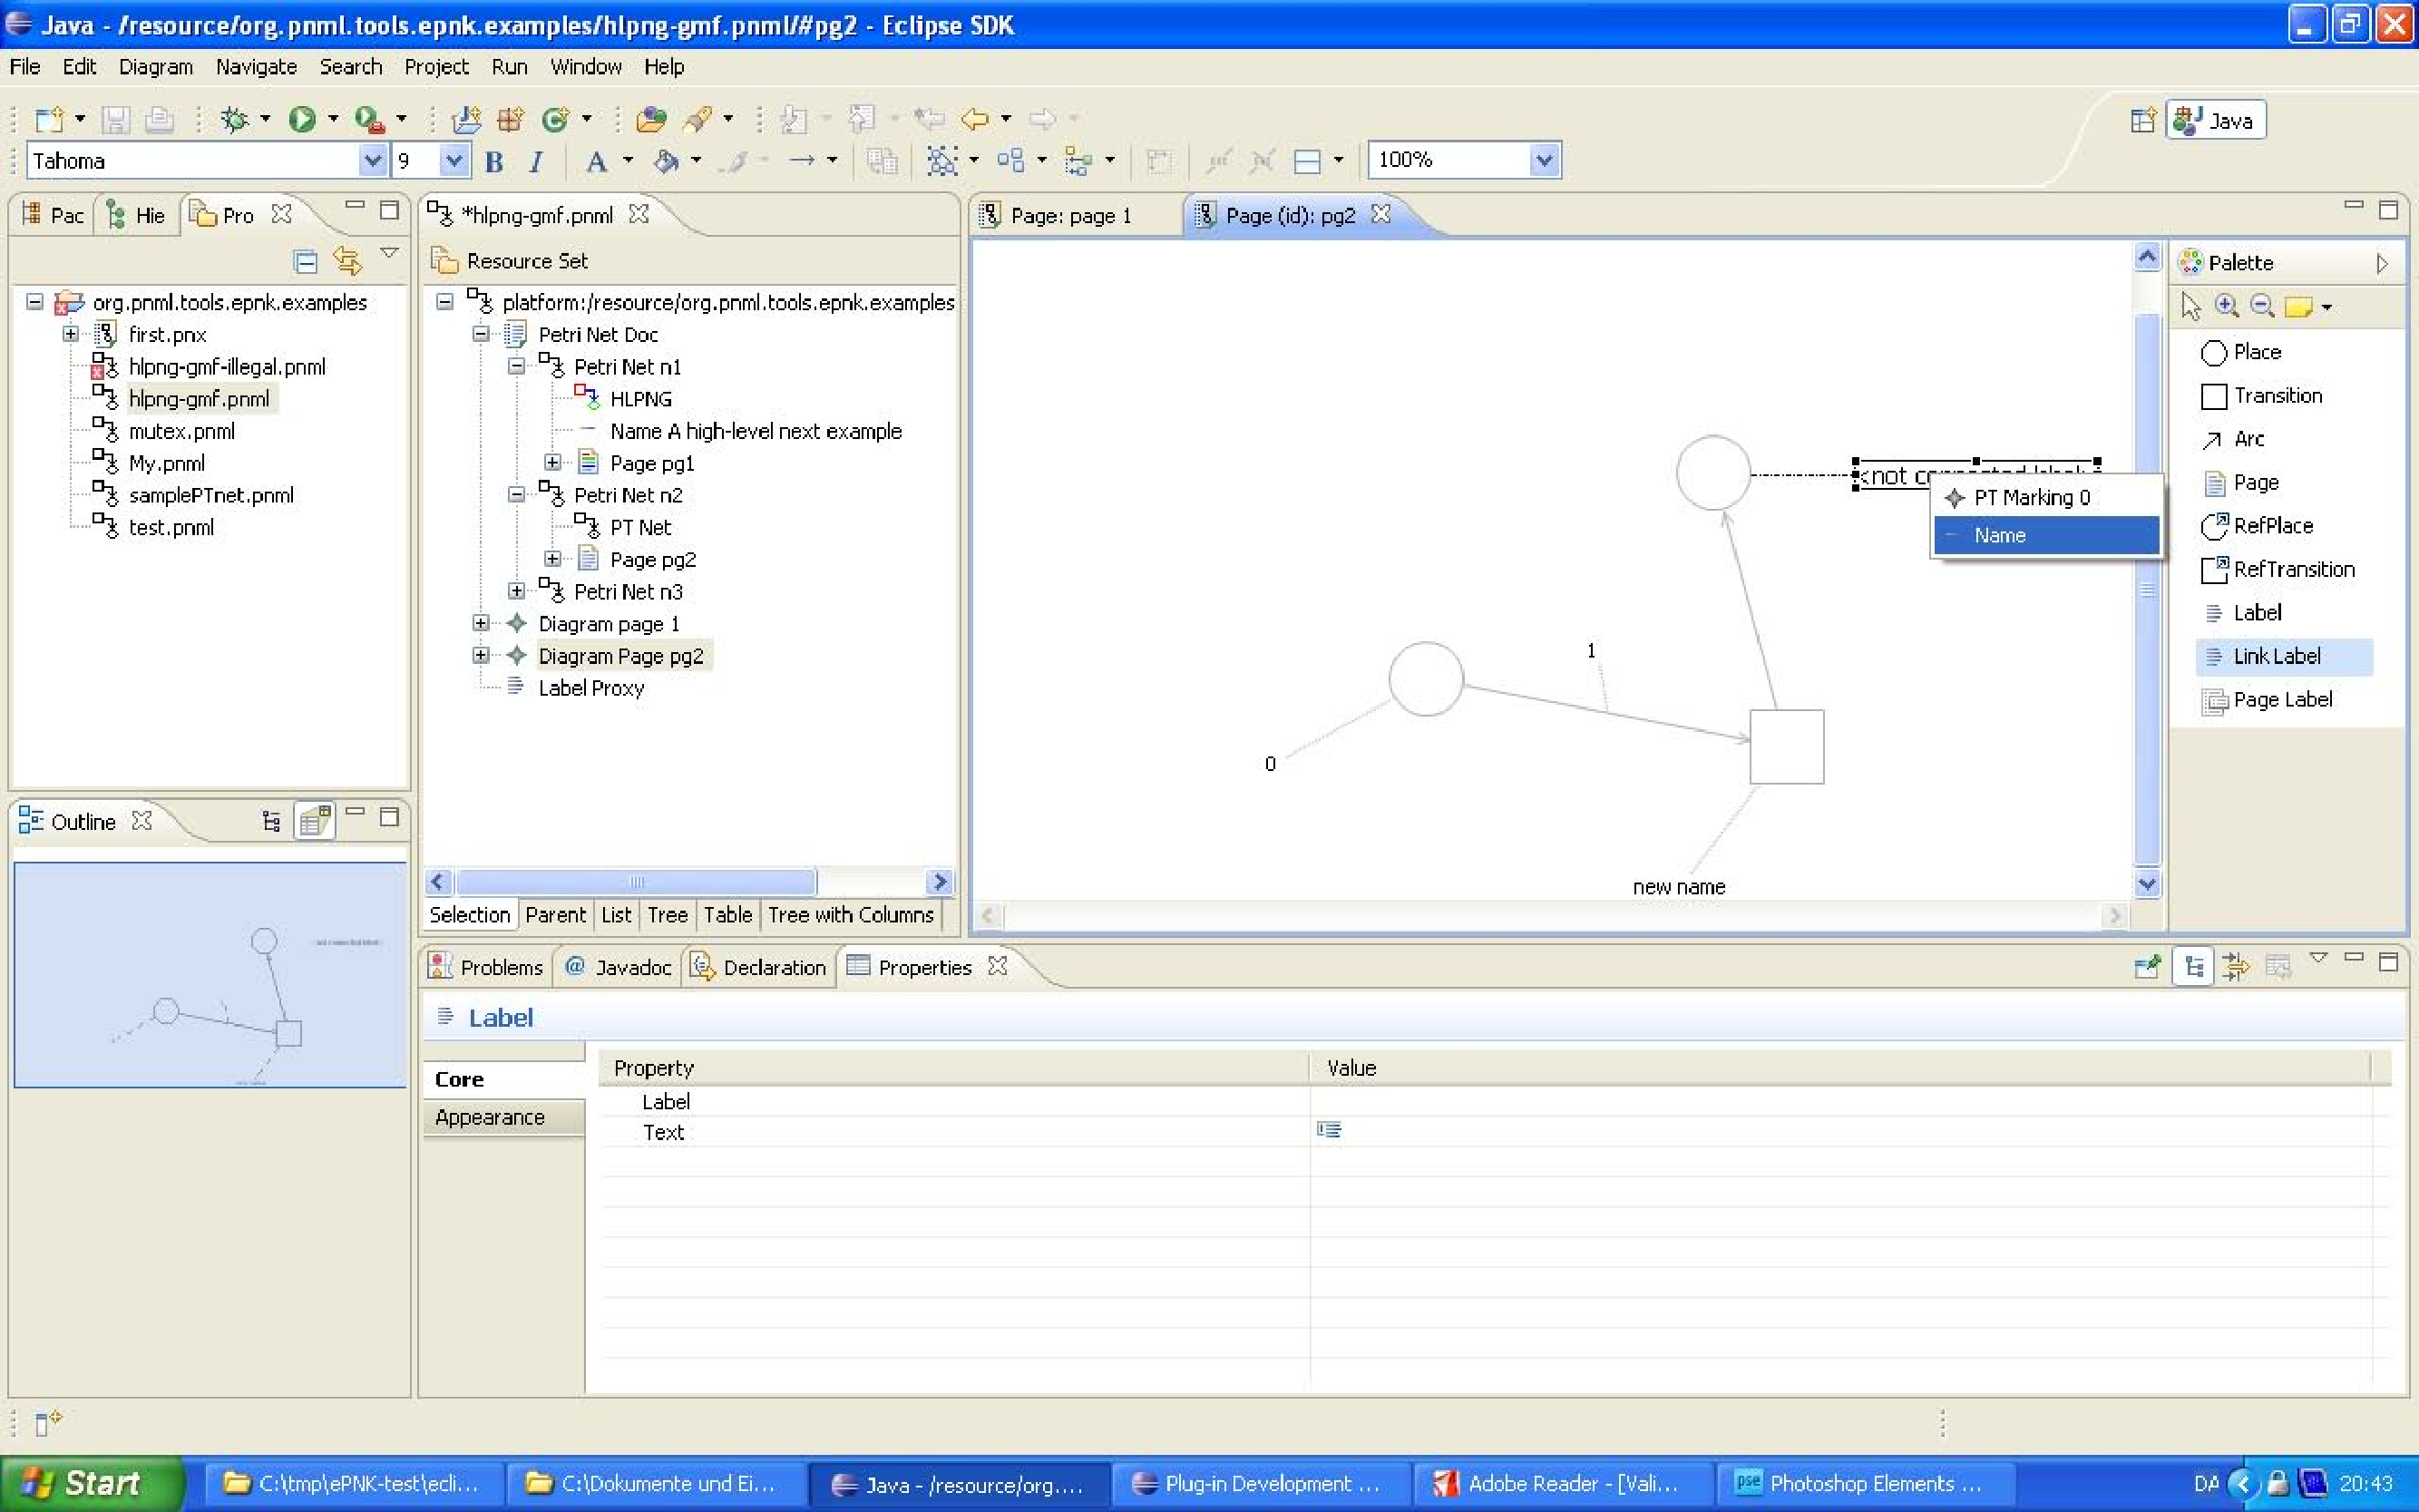
\includegraphics[scale=.25]{AttachLabel}}
  \caption{Pop-up menu during attaching a unconnected label to an object}
  \label{fig:label-connection}
\end{figure}

After the label has been attached to an object, it can be edited ``in place'',
by clicking into it and pressing the ENTER key in the end.  The legal syntax of
the label depends on the Petri net type and which kind of label it is. In
general, when editing labels and page labels there are two different
cases: The first case are \emph{simple labels},%
  \index{Label!Simple|DEF}
which typically are simple
values like ``true'' or ``false'', values like numbers, arbitrary strings,
or IDs (in general, it will be some form of data types). If such a label is
typed in syntactically incorrect, the new value will be rejected, and the
value of that label will be reverted to the value it had before editing. The
other case are \emph{structured labels}.%
  \index{Label!Structured|DEF}
These are, typically, labels with a
complex syntax, as for example the declarations of a high-level net (actually
all labels of high-level nets except for the names are structured). All these
labels will be parsed and checked for syntactical correctness; but the entered
text will be stored in all cases. If the text is syntactically incorrect,
however, the structure is not set and this will very likely result in some
validation%
  \index{ePNK!Validation}
error later (see Sect.~\ref{subsec:validation}). So this error needs to be
fixed, by editing the label again.  In case of such an error, the label will be marked
with a warning symbol (and when the mouse is moved over the warning symbol,
the tool tip will indicate that the label could not be parsed). If, for example,
we delete the comma that separates the two sort declarations in the label
``sorts B = (A*INT), C = (B*B);'' the label will be decorated with a warning
symbol. Upon validation, a validation error message will be given and later shown in the problems view.


The documentation of the legal syntax of these type specific labels, in
particular the one of the structural labels, is part of the documentation
of the Petri net type definition. For the types deployed together with the
ePNK, this information can be found in Sect.~\ref{sec:petrinettypes}.

Note that labels, in principle\footnote
 {That is, if the legal syntax of a specific Petri net type does allow it.}%
, can have line-breaks.  Since pressing the ENTER button will finish the
editing of a label, however, a line-break is inserted to a label by
pressing CNTRL-ENTER while editing the label.

Some Petri net types have quite many labels, and it is quite tedious to
create and link all these labels to a Petri net object. Therefore, the
graphical editor of the ePNK has a context menu when one of its objects
is selected, which will create and attach all missing default labels of that
object (and arrange them equally distributed around the object). The menu
pops up, when the right mouse button is pressed on the element; then select
``ePNK''$\rightarrow$``Add default labels''.%
  \index{ePNK!Add default labels@{Add default labels (menu)}|DEF}
  \index{Label|)}

\subsection{Attributes}
\label{subsec:attributes}

\index{Attribute|(DEF}
As discussed earlier, some ``labels'' of a Petri net object are not
supposed to be represented as graphical annotations of a Petri net object.
These are called \emph{attributes}.  Figure~\ref{fig:signal-net-attributes}
shows an example of a Petri net which uses attributes for some objects. It
is a signal-event net (SE-net)%
  \index{SE-nets}
\cite{StHa97}, which will be used later in the
Developers' Guide of this manual as an example of how to define new Petri net
types for the ePNK\footnote
  {The reason we need to resort to SE-nets here is that all the Petri net types
   that are defined in ISO/IEC~15909-2 use annotations only}. 

\begin{figure}[hbt!!]
  \centerline{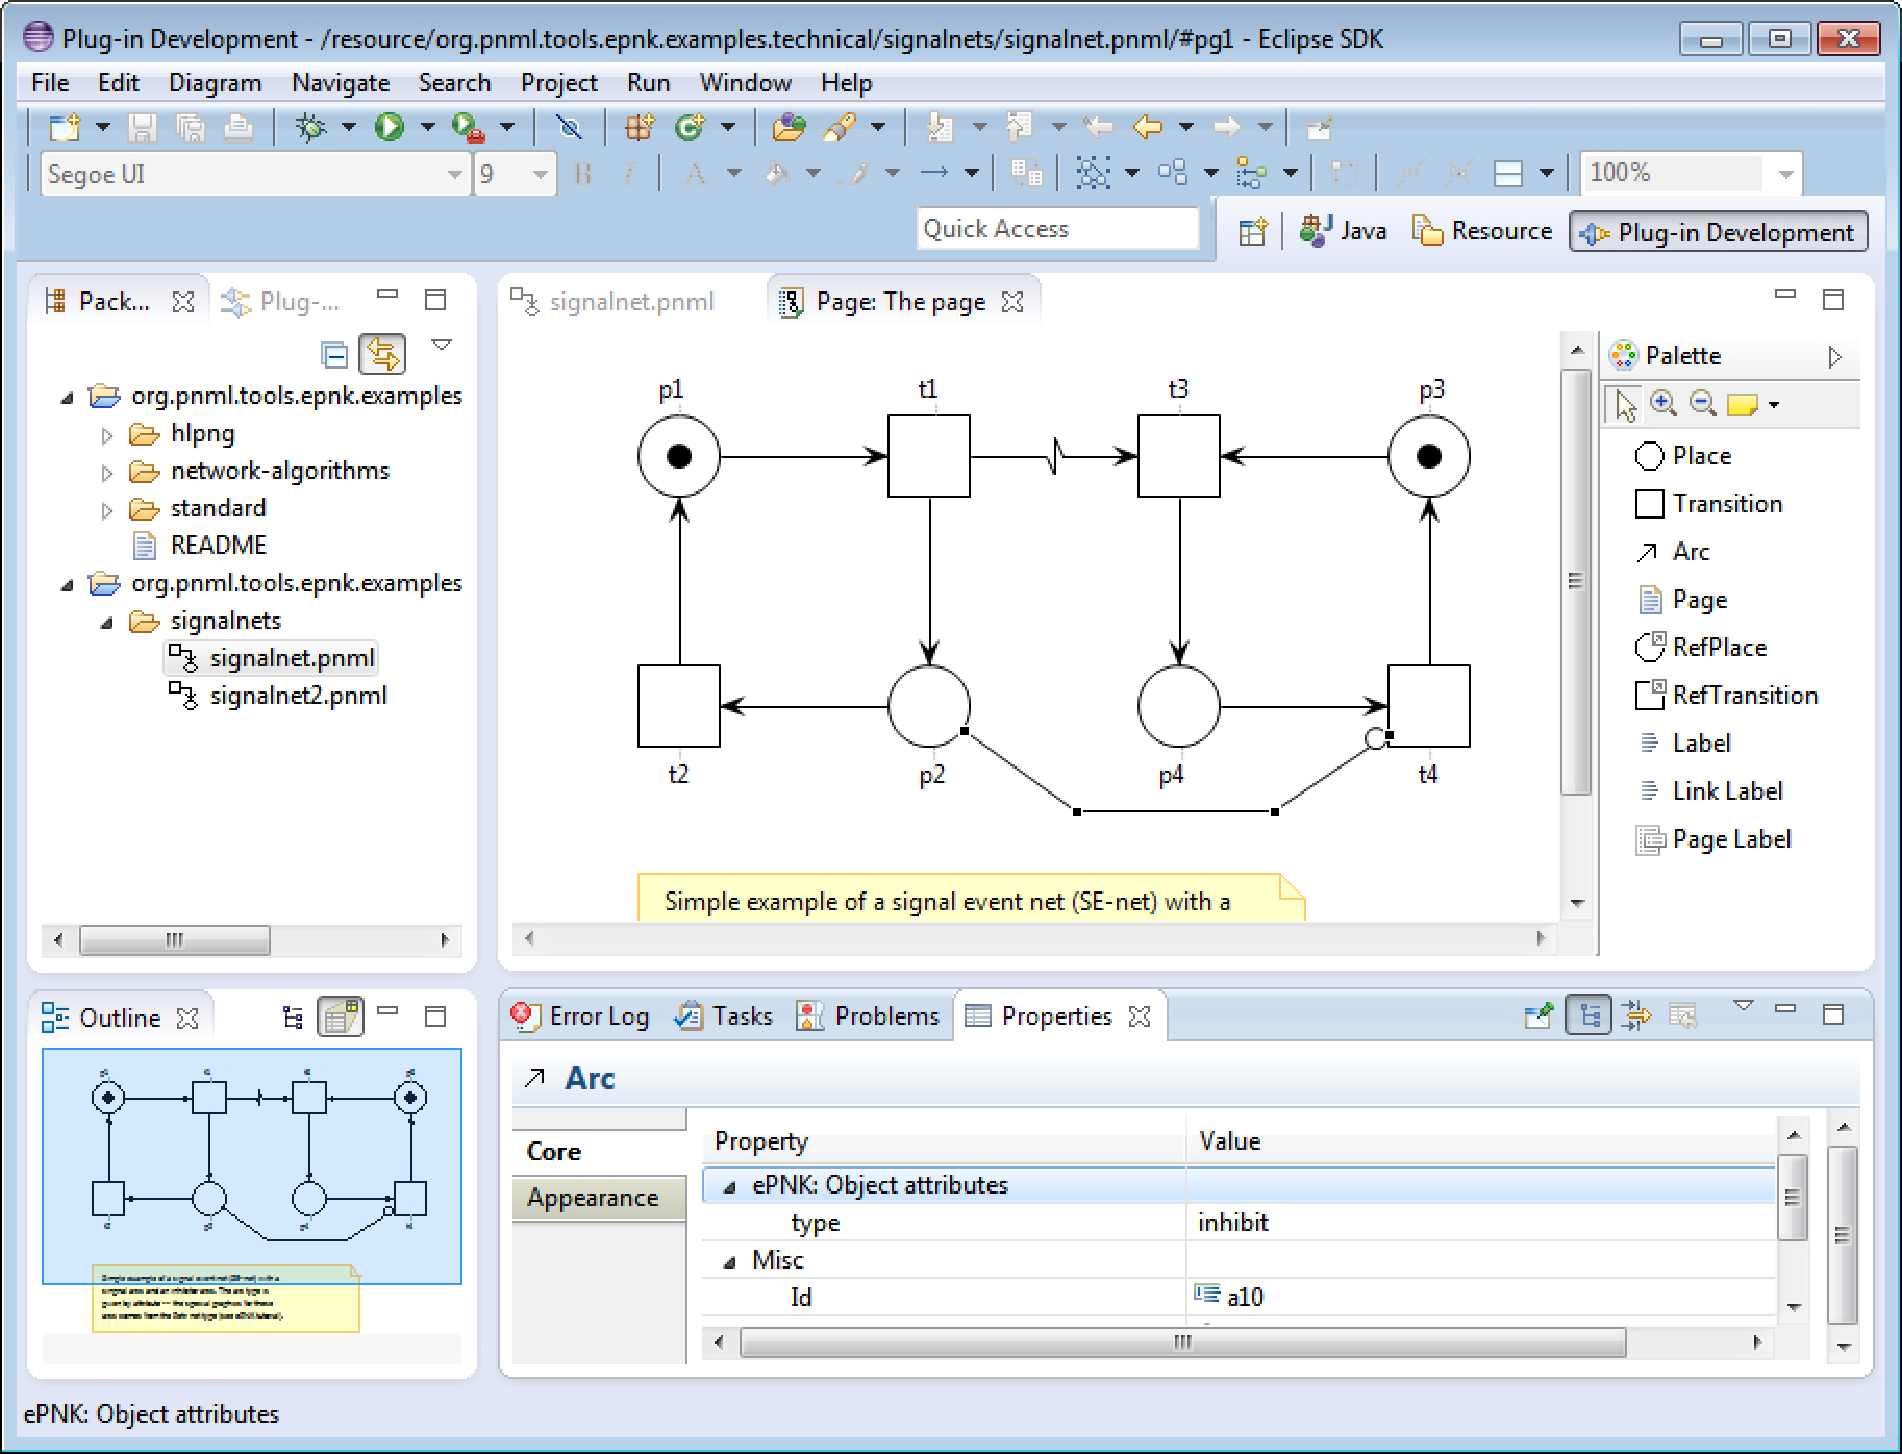
\includegraphics[scale=.38]{signalnet-attributes}}
  \caption{A Signal/Event net open in the graphical editor}
  \label{fig:signal-net-attributes}
\end{figure}

In this example, arcs have an arc type. If the arc type is not set, it is
considered to be a normal arc. The arc that is selected in
Fig.~\ref{fig:signal-net-attributes}, is of type ``inhibit'', i.\,e.\ it
represents an inhibitor arc. The value of the attribute is visible in
the properties view, and can also be changed there. In this example,
the arc is graphically shown as a lollipop -- which comes from the
implementation of that Petri net type, which implements a dedicated
graphical representation for these kind of arcs. Another
example is the signal arc (the one with the ``flash'' decoration), which is an
arc of type ``signal''. For this net type, we have chosen the marking to be an
attribute; therefore, the marking is not shown as a label. It can only be
changed by selecting the respective place, and then changing the
respective attribute in the properties view. In this net type, the marking
is indicated with a special graphics for the place (as black tokens).

As mentioned before, the value of an attribute can be changed by selecting the
respective object and then changing the value in the properties view.
Depending on the type of the attribute, this can be done by either typing
some text into the value column for that attribute or by a drop down menu
(if there are only finitely many possible values). If you want to reset
a value to the default value (the default is that the value is not set at all),
you can right-click into the property column of that property in the properties
view and then select ``Restore default value''.%
  \index{Attribute|)}

\subsection{Pages}
\label{subsec:sub-pages}
\index{Page|(DEF}

The graphical editor also allows you to create other pages on the
page it is showing. In order to avoid confusion, we call such
a page a \emph{sub-page}.%
  \index{Sub-page|DEF}
Creating a sub-page
can be done with the ``Page'' tool, in the very same way in which
places or transitions are created on a page. In the graphical editor,
a sub-page is graphically represented as a rounded rectangle. 

It is possible to open a graphical editor on a sub-page from the
graphical editor via a pop-up menu on the right mouse button: ``ePNK''
$\rightarrow$ ``Start GMF Editor on Page'' (as we have seen it for the tree
editor).
And also here, a double-click on the page in the graphical editor is
a shortcut for opening a graphical editor on this page.
Therefore, the tree editor is needed only for creating the top-level
pages of the net; all the sub-pages could be created by the
graphical editor. But navigation to sub pages might be a bit easier
and much faster in the tree editor; this is why you would probably want to use
the tree- editor for navigating and opening sub-pages further down in the
tree-hierarchy. It is recommended not to create sub-pages in the tree editor,
since they would not have a position in the graphical editor. Still, it is
possible and the graphical editor would show these pages (as well as other
objects created in the tree editor) in the top-left corner, when it is opened
with the graphical editor for the first time. Then, you could move it to
a better position.

The graphical editor indicates by a special decoration when a sub-page is
open in some graphical editor: a symbol of an open folder.

What is more important about pages is how to deal with their labels. Typically,
all the type-specific labels are represented as \emph{page labels}%
  \index{ePNK!Page label|DEF}
on the respective sub-page.
For HLPNGs, for example, the declarations of a page
are shown as page labels on that sub-page. The name, however, will be shown as a label
attached to that page on the super-page.  Which labels are shown as
labels attached to the sub-page on the super page, and which labels are shown
as page label on the opened sub-page is up to the Petri net type definition.%

Note that some Petri net types, allow labels to be directly defined for the net,
in which case they are \emph{net labels}%
  \index{ePNK!Net label|DEF}%
and not \emph{page labels}. This applies for example for all kinds
of declarations in High-level Petri nets (HLPNGs). Though, we do not recommend
to use them, ISO/IEC 15909-2 mandates tools to support them. The ePNL allows
to add net labels in the tree editor, if needed.

Note that even though, a Petri net can consist of many pages, the net is
considered as a single flat net only. \emph{Reference places}%
  \index{ePNK!Reference place}
and
\emph{reference transitions}%
  \index{ePNK!Reference transition}%
, are conceptually merged with the places and
transitions they refer to. This is what we call \emph{flattening of the net}.%
  \index{Flattening (of a net)|DEF}
In Sect.~\ref{subsubsec:developer:functitions:utilities:convenience} of the
Developers' Guide, we will see that the ePNK provides mechanisms for
accessing the flattened net structure in a uniform way.%
\index{Page|)}


\subsection{Graphical features}
\index{ePNK!graphical features|(DEF}

The graphical editor of the ePNK allows you to make all kinds of changes to
the graphical appearance of the Petri net. The features supported are
the standard features of GMF editors. Figure~\ref{fig:signal-net-graphics}
shows the same net as above again; in order to high-light some GMF features
now, the grid and rulers switched on.

\begin{figure}[hbt!!]
  \centerline{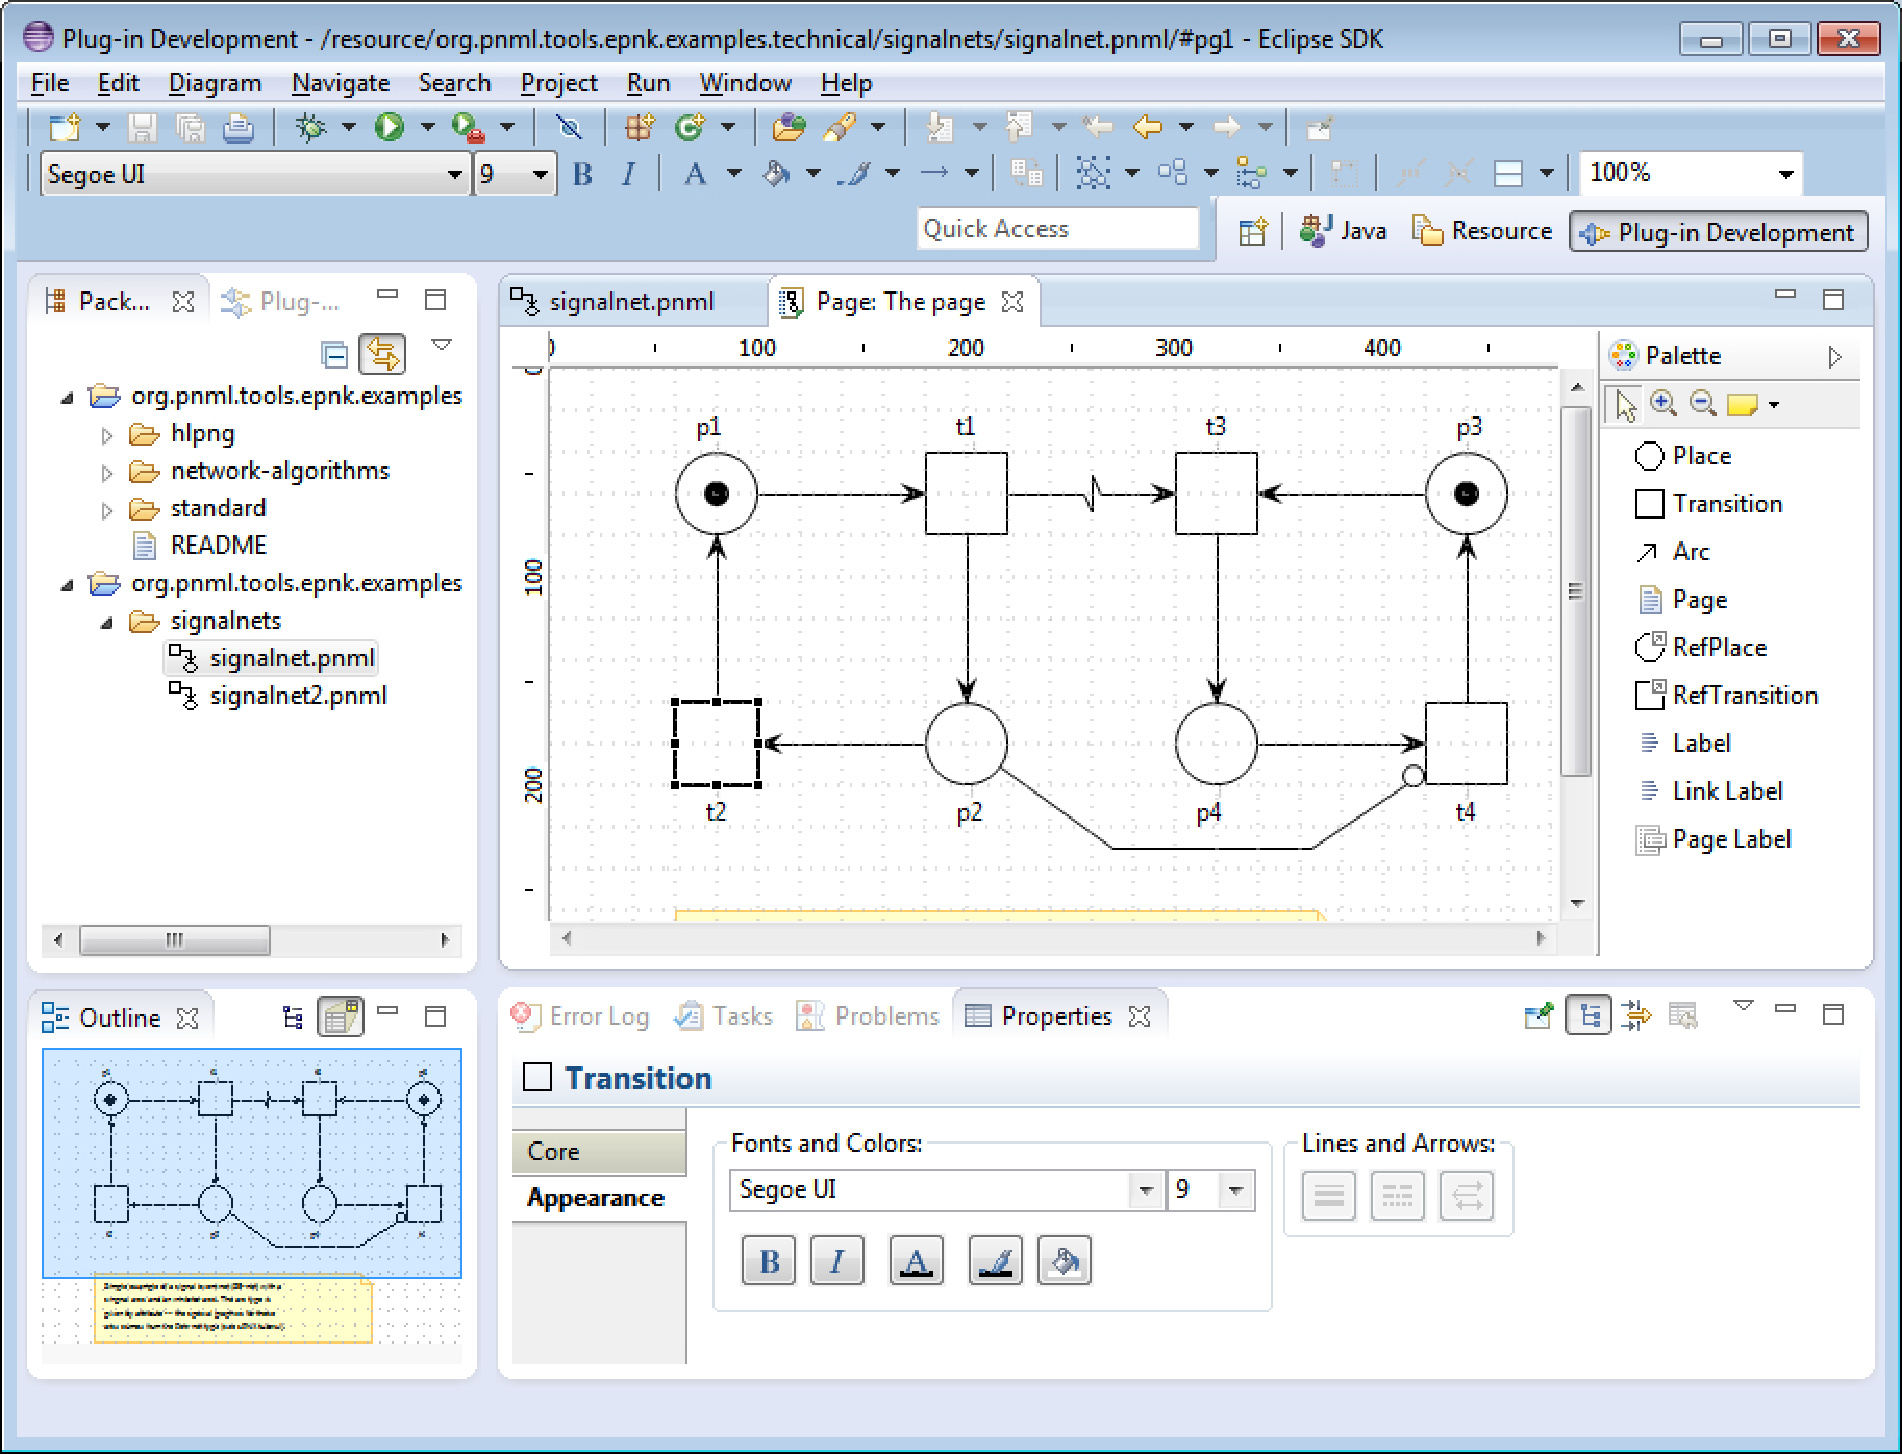
\includegraphics[scale=.38]{signalnet-graphics}}
  \caption{The Signal/Event net again: now with grid and rulers}
  \label{fig:signal-net-graphics}
\end{figure}

Since the graphical features are pretty straightforward, and are similar
to typical graphical editors, we do not explain the details here. The
graphical features can be changed in the properties view, when selecting
the ``Appearance'' section (up to now, the properties view had always
shown the ``Core'' section). Figure~\ref{fig:signal-net-graphics} shows
the graphical features that can be changed, when a node is selected. The
available features vary for the different kinds of objects.

Note that Petri net types can define a special graphical appearance for
some nodes or arcs, which depends on attributes or some other information
of the resp.\ element. In that case, some graphical information selected by
the user might be overruled by the specific graphical information for that
element of the Petri net type. You can see an example of such a specific
graphics in Fig.~\ref{fig:signal-net-graphics}, where signal arcs and
inhibitor arcs are shown in their usual graphical notation. In this example,
however, the specific graphical information does not interfere with the
user graphics. But, if a net type defines that some specific arcs should
be displayed in red colour, for example, this would override the colour chosen
by the user.

The ePNK saves the nets in exactly the graphical representation you
see them before you save the file. But, the exact graphical representation
is saved as a tool specific extension of the ePNK! This means that the
exact graphical representation can be reproduced in the ePNK only.

The ePNK also transfers most of the graphical information to the respective
features of PNML, so that other tools could reproduce almost the same
graphical appearance as you see it in the ePNK. Some features, however,
are not supported by PNML (as for example the size of labels) and some
others are not yet transferred by the ePNK to PNML. In turn, some graphical
features of PNML are not supported by the ePNK editor (e.\,g.\ the alignment
of text in labels).

In Sect.~\ref{subsec:supported-graphical-features}, you will find a complete
list of graphical information that is transferred to PNML elements. Here
is a brief list of graphical information from the graphical ePNK editor
that is \emph{not} transferred to PNML: font styles (bold or italic for labels);
routing and jump link information for arcs. Note that also the comments that
you can place on a page will be lost in other tools, since this is tool specific
information only in the ePNK (comments are not a concept of PNML).

Note that PNML nodes that do not have a size attached to them, will have the
width and height 40pt in the ePNK (which the GMF default). 

Arcs can have \emph{intermediate points} or \emph{bend points}%
  \index{intermediate point|DEF}%
  \index{bend point|DEF}
in the ePNK as well as in the PNML. These intermediate points will be
transferred to the PNML model. But there is some caveat: when a node is moved in
the ePNK editor, the bend points of the attached arcs might also be moved. Due
to some quirk in GMF, these changes are not transferred to the PNML model at
all. If you want to be sure that the intermediate points of the PNML model
corresponds to what you see in the graphical editor of the ePNK, you should
move at least one bend point of each arc attached to the node after you have
moved the node.

Arcs are either drawn as a \emph{polyline} or as a \emph{bezier curves}, which
is defined by the ``Smoothness'' chosen for the respective arc in the ePNK
editor. The ePNK draws an arc as a polyline, if the ``Smoothness'' is%
  \index{Smoothness (of an arc)|DEF}%
  \index{Curved arc|DEF}%
  \index{Polyline arc|DEF}
set to ``None''; for all other choices of ``Smoothness'' (i.\,e.\ ``Normal'',
``Less'', or ``More'') the arc will be drawn as a quadratic bezier curve,
where every second intermediate point is used as a control point as mandated
by ISO/IEC~15909-2. The information on whether an arc should be drawn as a
straight line or as a bezier curve is transferred to the PNML model.
 
\index{Image|(DEF}
The graphical editor of the ePNK also supports the \emph{image} feature of PNML:
Every node can be assigned an image in the PNML model; instead of the 
normal shape of the respective node, the image will be shown. The ePNK
supports JPEG and PNG -- as required by PNML. Actually, the ePNK supports
even more image formats\footnote
  {All image formats supported by the Eclipse SWT {\tt ImageLoader}
   should work: BMP, ICO, JPEG, GIF, PNG and TIFF.}%
. But, since the other formats are not supported by PNML, we recommend
to use the JPEG and PNG format only.

% Right now, the image attribute of a node (in the Fill element of the
% NodeGraphics) can be set in the tree editor only. From version~1.0.1 on, 
The properties view has an image property, in which the path to the image
can be set directly when the resp.\ element is selected in the graphical editor.
The paths should be a relative path to the image, staring from the folder that
contains the PNML document.

Note that, for efficiency reasons, each image is loaded only once -- the first
time it needs to be shown in the graphical editor. If you change an
image file and you want a graphical editor in an already open document to
show the new image, the \emph{image cache}%
  \index{ePNK!Image cache|DEF}
of the open editor must be cleared
explicitly. To this end, right-click on the top-level ``Petri Net Doc''
element in the ePNK tree editor of that document and select
``ePNK$\rightarrow$``Clear Image Cache''.%
  \index{ePNK!Clear image cache|DEF}
  \index{Image|)}%
  \index{ePNK!graphical features|)}%
  \index{ePNK!Graphical editor|)}%

\section{Petri net types} 
\label{sec:petrinettypes}
\index{PNTD|DEF}

In this section, we give an overview of the Petri net types that are
deployed together with the ePNK. In the basic version of the ePNK, these
are \emph{P/T-Systems} (\emph{PTNet})%
  \index{P/T-Systems|DEF}
  \index{ePNK!PTNet|DEF}
and \emph{high-level Petri nets} (\emph{HLPNG}).%
  \index{High-level Petri nets|DEF}
  \index{ePNK!HLPNG|DEF}
Moreover, there is the \emph{empty type} (\emph{Empty}),%
  \index{Empty (net type)|DEF}
which, however, does not contain any concepts in addition to the
PNML core model; therefore, we do not discuss the empty type here. The empty
type was introduced to explicitly indicate, that there are no Petri net type
specific extensions. 

Actually, HLPNGs come in different levels or kinds: ``\emph{dot nets}'',%
  \index{ePNK!Dot net|DEF}
which are a way of representing P/T-Nets as high-level nets; basically, ``dot
nets'' are high-level nets restricted to the sort ``DOT'' and a minimal version of
operators on them; ``\emph{symmetric nets}''%
    \index{ePNK!Symmetric net|DEF}
are a restricted version of
high-level nets that uses  some special finite sorts and a limited set of operations only;
and the full version of high-level nets. The kind of a HLPNG can be
changed by selecting the HLPNG type in the tree editor and by selecting the kind
attribute in the properties view (identified by the respective URI as defined by
ISO/IEC~15909-2).
For a detailed discussion of the legal constructs of the different kinds of HLPNG,
we refer to the discussion of ISO/IEC 15909-2 \cite{HKea09}. Note that, in
contrast to the Petri net type, the kind of a HLPNG can be manually changed anytime, since the kind of HLPNG
concerns the validation only. The PNML syntax is the same.

\subsection{PTNet}
\label{subsec:PTNet}
\index{ePNK!PTNet|(DEF}

We start with explaining the details of \emph{PTNets}. In
Sect.~\ref{subsec:PNTD} we have already seen the additional features of 
PTNets, which are the initial marking for
places and the inscription for arcs. Both labels are simple labels, which
means that it will be checked right after editing a label whether the label is
syntactically correct (see Sect.~\ref{subsec:labels}); if it is not
correct, the value will be reverted to the value it had before.

The marking of a place must be a non-negative integer in any reasonable
representation\footnote
 {For those who want to bother with the technical details, it can be any
  String that would be accepted by the Java {\tt Integer.parseInt()}
  method as a number and that evaluates to a number greater or equal than 0.}%
.  The arc-inscription is similar, just that it must represent a positive 
integer (i.\,e.\ must be a number greater than 0).

Moreover, PTNets have the restriction that arcs may only run from a
place to a transition or from a transition to a place, which will
be enforced in the graphical editor\footnote
  {In the tree editor, illegal arcs can be created, but the respective net
   would not pass validation.}%
. Actually, the constraint is slightly more complicated due to
reference nodes: We can connect place-like nodes (PlaceNodes)
with transition-like nodes (TransitionNodes) and vice versa;
but semantically, i.\,e.\ when flattening a net (see
Sect.~\ref{subsec:sub-pages}), this amounts to the above condition.%
  \index{ePNK!PTNet|)}

\subsection{HLPNG}
\label{subsec:introHLPNG}
\index{HLPNG|(DEF}

\emph{HLPNGs} are much more involved than P/T-Nets and we cannot explain
them in all details here. For a detailed motivation and full account
on what \emph{HLPNGs} are, we refer to ISO/IEC~15909-2
\cite{ISO-IEC:15909-2-2011,HKea09}. Actually, HLPNG are
conceptually quite close to coloured Petri nets \cite{JeKr09} or
algebraic system nets \cite{KiRe96}.

For HLPNGs, there are the following labels (in addition to names):
\begin{description}
  \item[Declaration] A \emph{declaration}%
       \index{Declaration|DEF}%
is a page label, which is used
     to define \emph{variables}%
       \index{Varialble|DEF}%
, \emph{sorts},%
       \index{Sort|DEF}%
     and \emph{operators}%
         \index{Operator|DEF}%
, which can then be used in the other labels.  Every page can have
     any number of declarations and, within a single declaration,
     different kinds of declarations can be mixed. Note that all
     declarations are global (known in the complete Petri net),
     even though they are attached to a specific page.
     
     Declarations do not need to be contained in a page at all --
     they can be contained directly in the net. We do not recommend
     to make use of that; but ISO/IEC~15909-2 mandates
     this to be possible. So, the ePNK can read nets with declarations
     which are directly contained in the net and such net labels can
     be created in the tree editor of the ePNK, if needed.

  \item[Type] A \emph{type}%
       \index{Type|DEF}
     is a label that is associated with a place.
     Every place must have exactly one type label which denotes
     the sort of the tokens on that place. This sort can be built
     from the predefined sorts of HLPNGs or some user-defined sorts.

  \item[HLMarking] A \emph{marking}%
       \index{Marking|DEF}
     is a label that is attached to a place
     and defines the place's initial marking. The marking is
     represented by a ground-term\footnote
      {A ground-term is a term that does not contain variables.},
     which must denote a multiset over the place's type. Note that this
     label may be omitted, in which case the initial marking is
     considered to be empty. There can be at most one label of this
     kind.

  \item[Condition] A \emph{condition}%
       \index{Condition|DEF}
     is a label that can be attached
     to a transition. The condition is a term of type boolean and
     can contain variables. There can be at most one condition;
     if the condition is missing, it is assumed to be true.

  \item[HLAnnotation] An \emph{arc annotation}%
       \index{Arc annotation (HLPNGs)|DEF}
     is also a term that may
     contain variables. The term must be a multiset term over the
     type of the place to which the arc is attached. Every arc should
     have exactly one arc annotation\footnote
     {Actually, ISO/IEC~15909-2 would allow that this label is
      missing. This does not make much sense though since, in most cases,
      there is no reasonable standard interpretation if the label is
      missing.}.
\end{description} 

All labels of HLPNGs are structural labels (see Sect.~\ref{subsec:labels}),
which means that the user can edit them and leave them syntactically incorrect.
Of course, this will not pass validation; but, it is possible to save
nets with incorrect labels and load them again, so that the labels can
be corrected another time.

PNML does not define or mandate a concrete syntax for declarations and terms.
The concrete syntax for the labels is up to each tool; so it might be different
in different tools. What matters is the abstract syntax. In order to, get
the abstract syntax of a HLPNG net of some net from another tool into the
concrete representation of the ePNK, the ePNK provides a pop-up action,
which converts the abstract syntax into ePNK's concrete syntax. It is
available in the tree editor\footnote
  {Note that you must have installed the ``HLPNG Label Serialisation'' feature
   for this to work.}%
, when a HLPN object is selected ``ePNK''$rightarrow$``Serialise HLPNG
Labels''.%
  \index{HLPNG Label Serialisation|DEF}

ePNK's concrete syntax for HLPNG labels resembles the one of CPN Tools
\cite{JeKr09}, but it is not identical to the one of CPN Tools! Below, we
explain this ePNK's concrete syntax for labels. Before going into the details
of the syntax, we briefly discuss some examples.

The following shows several declarations of variables, sorts and operators.
Each of them could be in a separate declaration label, but they could also be
contained in a single declaration:
\begin{verbatim} 
vars
  x:NAT;
  
sorts
  A = MS(BOOL);
  
ops
  f(x:INT, y:INT) =  x * y,
  g() = 1;
  
sorts B = (A*INT), C = (B*B);    
\end{verbatim}

First, a variable x of built-in sort NAT is defined. Then a user-defined
sort A is defined, which is a multiset over the built-in sort BOOL. Then,
two named operations are defined, f and g. The operation f takes two parameters
of type INT; the operation g does not have parameters. Note that named
operations, basically, are abbreviations and, therefore, do not allow any
recursion (see \cite{HKea09} for details). In the end, two other user-defined
sorts are defined: B is a product of A and the built-in sort INT, and C is a pair over
sort B. Note that also for sort declarations, recursion is not allowed.

The right-hand sides of the sort declarations above give you an idea of the
syntax for sorts already. There are some built-in sort like BOOL, INT, NAT, POS and
DOT. From these, we can built products or multiset sorts.

Here are some examples of terms (using the above declarations):
\begin{verbatim}
 x`f(x,x) ++ 1`x ++  x`g() ++  1`5
 
 1`(dot,1) ++ 1`(dot,1*1)
 
 x > 1 and x < 5 
\end{verbatim}
The first is a multiset term over the sort INT, which could be used in
arc inscriptions (if the attached place is of type INT). The second is
a ground term over the product of built-in sort DOT with INT, where DOT is
a sort that represents a type with a single element dot. The last term
is a term of sort BOOL, which could be used as a condition.

The precise syntax is defined by the following grammar (that actually is
a simplified version of the grammar that was used for generating the parser).
The terminals ID, INT, NAT, STRING in this grammar represent legal identifiers
and legal representations of integer numbers, non-negative integer numbers
and string constants.

Listing~\ref{lst:grammar1} shows the part of the grammar for declarations.
\begin{figure}[htbp!]
\lstinputlisting[label=lst:grammar1,stringstyle=\normalsize,%
caption={Grammar for declarations}]%
  {HLPNGInscriptionLanguage.xtext}
\end{figure} 
%
Listing~\ref{lst:grammar2} shows the part of the grammar for terms.
\begin{figure}[htbp!]
\lstinputlisting[label=lst:grammar2,stringstyle=\normalsize,%
caption={Grammar for terms}]%
  {HLPNGInscriptionLanguage2.xtext}
\end{figure}
Note that we have simplified the grammar for making it more readable. The
simplification, however, makes the grammar ambiguous (i.\,e.\ some texts could be
parsed in two or more different ways). The ambiguities can be resolved again by
assigning a binding priority to the different operators -- moreover all operators are left-associative.
Each line in the declaration of BinOp represents operators on the same
level of priority, where the first line has the least binding-power and
the last the highest. The unary operators (actually there is only one) have the
highest binding power of all. Note that there are also some operators like the
cardinality, which use circumfix notation: if m is some multiset  \verb+|m|+
denotes the cardinality of that multiset. This operator has the same binding
power as parentheses.

Listings~\ref{lst:grammar3} and~\ref{lst:grammar4} show the part of the
grammar for built-in sorts and constants.
\begin{figure}[htbp!]
\lstinputlisting[label=lst:grammar3,stringstyle=\normalsize,%
caption={Grammar for sorts and constants (1)}]%
  {HLPNGInscriptionLanguage3.xtext}
\end{figure} 
%
\begin{figure}[htbp!]
\lstinputlisting[label=lst:grammar4,stringstyle=\normalsize,%
caption={Grammar for sorts and constants (2)}]%
  {HLPNGInscriptionLanguage4.xtext}
\end{figure} 
Note that every number constant will implicitly be assigned the tightest fitting
sort: INT, NAT, or POS. If a positive integer, say 5 should have the type
INT instead, this can be expressed by 5:INT, which works like a type cast in
object-oriented programming languages.

In addition to these syntactical constraints, the terms must also be correctly
typed, which we do not discuss here in detail. 

For HLPNGs, there are many constraints. Like for PTNets, arcs may only
run from places to transitions or from transitions to places. All of the
other additional constraints concern the correctness of the labels of
HLPNGs. The following list gives an overview:
\begin{enumerate}
  \item Every place must have a correct type (a correct sort in the context of
        the defined sorts of the net).
  \item Every declaration must be syntactically correct and correctly typed.
  \item Every declaration must properly resolve (must not be recursive and all
        symbols it refers to must be defined).
  \item Every term (in markings, arc annotations, and conditions) must
        be syntactically correct and correctly typed.
  \item The marking of a place must be a ground term and must be
        a multiset over the sort of the place.
  \item The arc annotation must be a term that is a multiset over the
        attached place's sort.
  \item Every condition must be a term of sort BOOL.
  \item Every declaration should have a distinct name (actually, this causes a
        warning only since this is a condition on concrete syntax, which is not
        part of PNML).
  \item The parameters of every operation declaration should have distinct names
        (actually, this causes a warning only since this is a condition
        on concrete syntax, which is not part of PNML). 
\end{enumerate}

As mentioned earlier, PNML and ISO/IEC~15909-2 do not define a concrete
(textual) syntax for declarations and terms. The syntax defined here is a syntax
specific to the ePNK. In principle, a PNML document with a high-level Petri net in
it could leave all the textual parts of the labels empty. In that case,
the most important structure and content of these labels would not be
visible in the graphical editor at all. The user would not see and would not
be able to edit the labels textually. In order to convert this structural
information into some text that can be edited by the user in the ePNK, a
simple extension to the ePNK is deployed as a separate feature called ``HLPNG
Label Serialisation''. % It is recommended to install this feature.
%
If you have the ``HLPNG Label Serialisation'' feature installed, you can
serialize all structured labels to the textual syntax of the ePNK. To this
end, right-click on the respective HLPN element (the Petri net) in the
tree editor; then select ``ePNK''$\rightarrow$''Serialise HLPNG Labels''.%
  \index{HLPNG Label Serialisation|DEF}%
  \label{sec:user:hlpng:label-serialisation}%
  \index{HLPNG|)}%
Then, you will be able to see and edit the labels in the syntax that we
have discussed above (independently from which editor the PNML file came from).

\subsection{Other types}

Note that there are some other Petri net types coming with the ePNK, if
if you have the ePNK tutorial installed.  Most notably, there are
\emph{Signal/Event-systems} (\emph{SE-Nets})%
  \index{Signal/Event-systems}
  \index{SE-nets}%
, which we will use as an example later in the Developers' Guide (see
Chapt.~\ref{chap:developers-guide}). Moreover, there is a technical
Petri net type where pages and arcs are equipped with comments, and
arcs can have different types. This type is called \emph{ArcTypes}, but
mainly serves as a tutorial for using attributes, and for equipping
a net with graphical extensions.

If you have the ECNO extensions installed, you have so-called ECNO nets,
which allow to model the life-cycle of elements in the so-called \emph{Event
Coordination Notation}. These are a story of their own \cite{Kin14a} and are not
discussed here.

\section{Functions and Applications}
\label{sec:users-guide:applications}
  \index{ePNK!Function|(DEF}%
  \index{ePNK!Application|(DEF}%
  
The ePNK in its basic version does not come with much functionality for
analysing, simulating and verifying Petri nets. Its main purpose, is
to provide a graphical editor for Petri nets and PNML Documents, and
to provide an infrastructure so that new Petri net types and new functions
and applications for Petri nets can be plugged in. By and by, some functions
have been developed that are now deployed together with the ePNK. And there
are some applications of the ePNK, which are projects in their own right -- for
example the ECNO project, which generates code for so-called ECNO nets
\cite{Kin12b}. We hope, that over time, more functions and applications
of other ePNK developers will be deployed together with the ePNK.

In this section, we explain some of the basic functions and applications
that are deployed together with the ePNK. In these examples, we will
also explain the \emph{ePNK applications view},%
  \index{ePNK!Applications view}
which is used as a
general user interface for the end user to control ePNK applications. 
Later, in the Developers' Guide in Chapt.~\ref{chap:developers-guide}, we
explain how you can contribute your own functions and applications to the ePNK.

Generally, the ePNK distinguishes \emph{functions} and \emph{applications}.
A \emph{function}
is something, which is initiated on some Petri net, possibly asking the user for
some extra input, then does some computation, and when the computation is
finished, provides some output to the user in form of some dialog. After that,
the function and its result are gone. One example of such a function is the
verification of some CTL formula for some Petri net by a model checker, which
is discussed in Sect.~\ref{subsec:user:model-checker}. In particular, the
model checker does not show or visualize any result in the Petri net itself.
Also an \emph{application}
is initiated on some net. In contrast to a function, the application
has a longer live-time, it shows some feedback to the user on top of the
Petri net in the graphical editor, and also provides means for the user
to interact with the application. An example of such an application is a 
simulator for high-level Petri nets, which is discussed in
Sect.~\ref{subsec:user:hlpng-simulator}. This simulator shows
graphically which transitions are currently enabled, and, by clicking
on them, the user can determine which transition should fire next.%
  \index{ePNK!Function|)}%
  \index{ePNK!Application|)}%

\subsection{A simple model checker for EN-systems}
\label{subsec:user:model-checker}
\index{Model checker|(}

In this section, we briefly discuss how to use the \emph{model checker}, which
can be initiated on P/T-nets. Note that even though this model checker
is initiated on P/T-nets, the model checker interprets the net as
an Elementary Net System (EN-systems) \cite{Thi87,Roz87}, which means
that at any time on any place, there can be at most one token.
A transition that would add another token to a place, would not be
able to fire -- and all arc-inscriptions are ignored.

Figure~\ref{fig:user:multi-agent} shows a P/T-net which consists
of several pages. Page {\sf pg0} (not visible) contains
a single place {\sf semaphor} with one initial token, and pages
{\sf pg1}, {\sf pg2}, and {\sf pg3} model three agents with the same
life-cycle, which is shown in the graphical editor in
Fig.~\ref{fig:user:multi-agent}.
%
\begin{figure}[hbt!!]
  \centerline{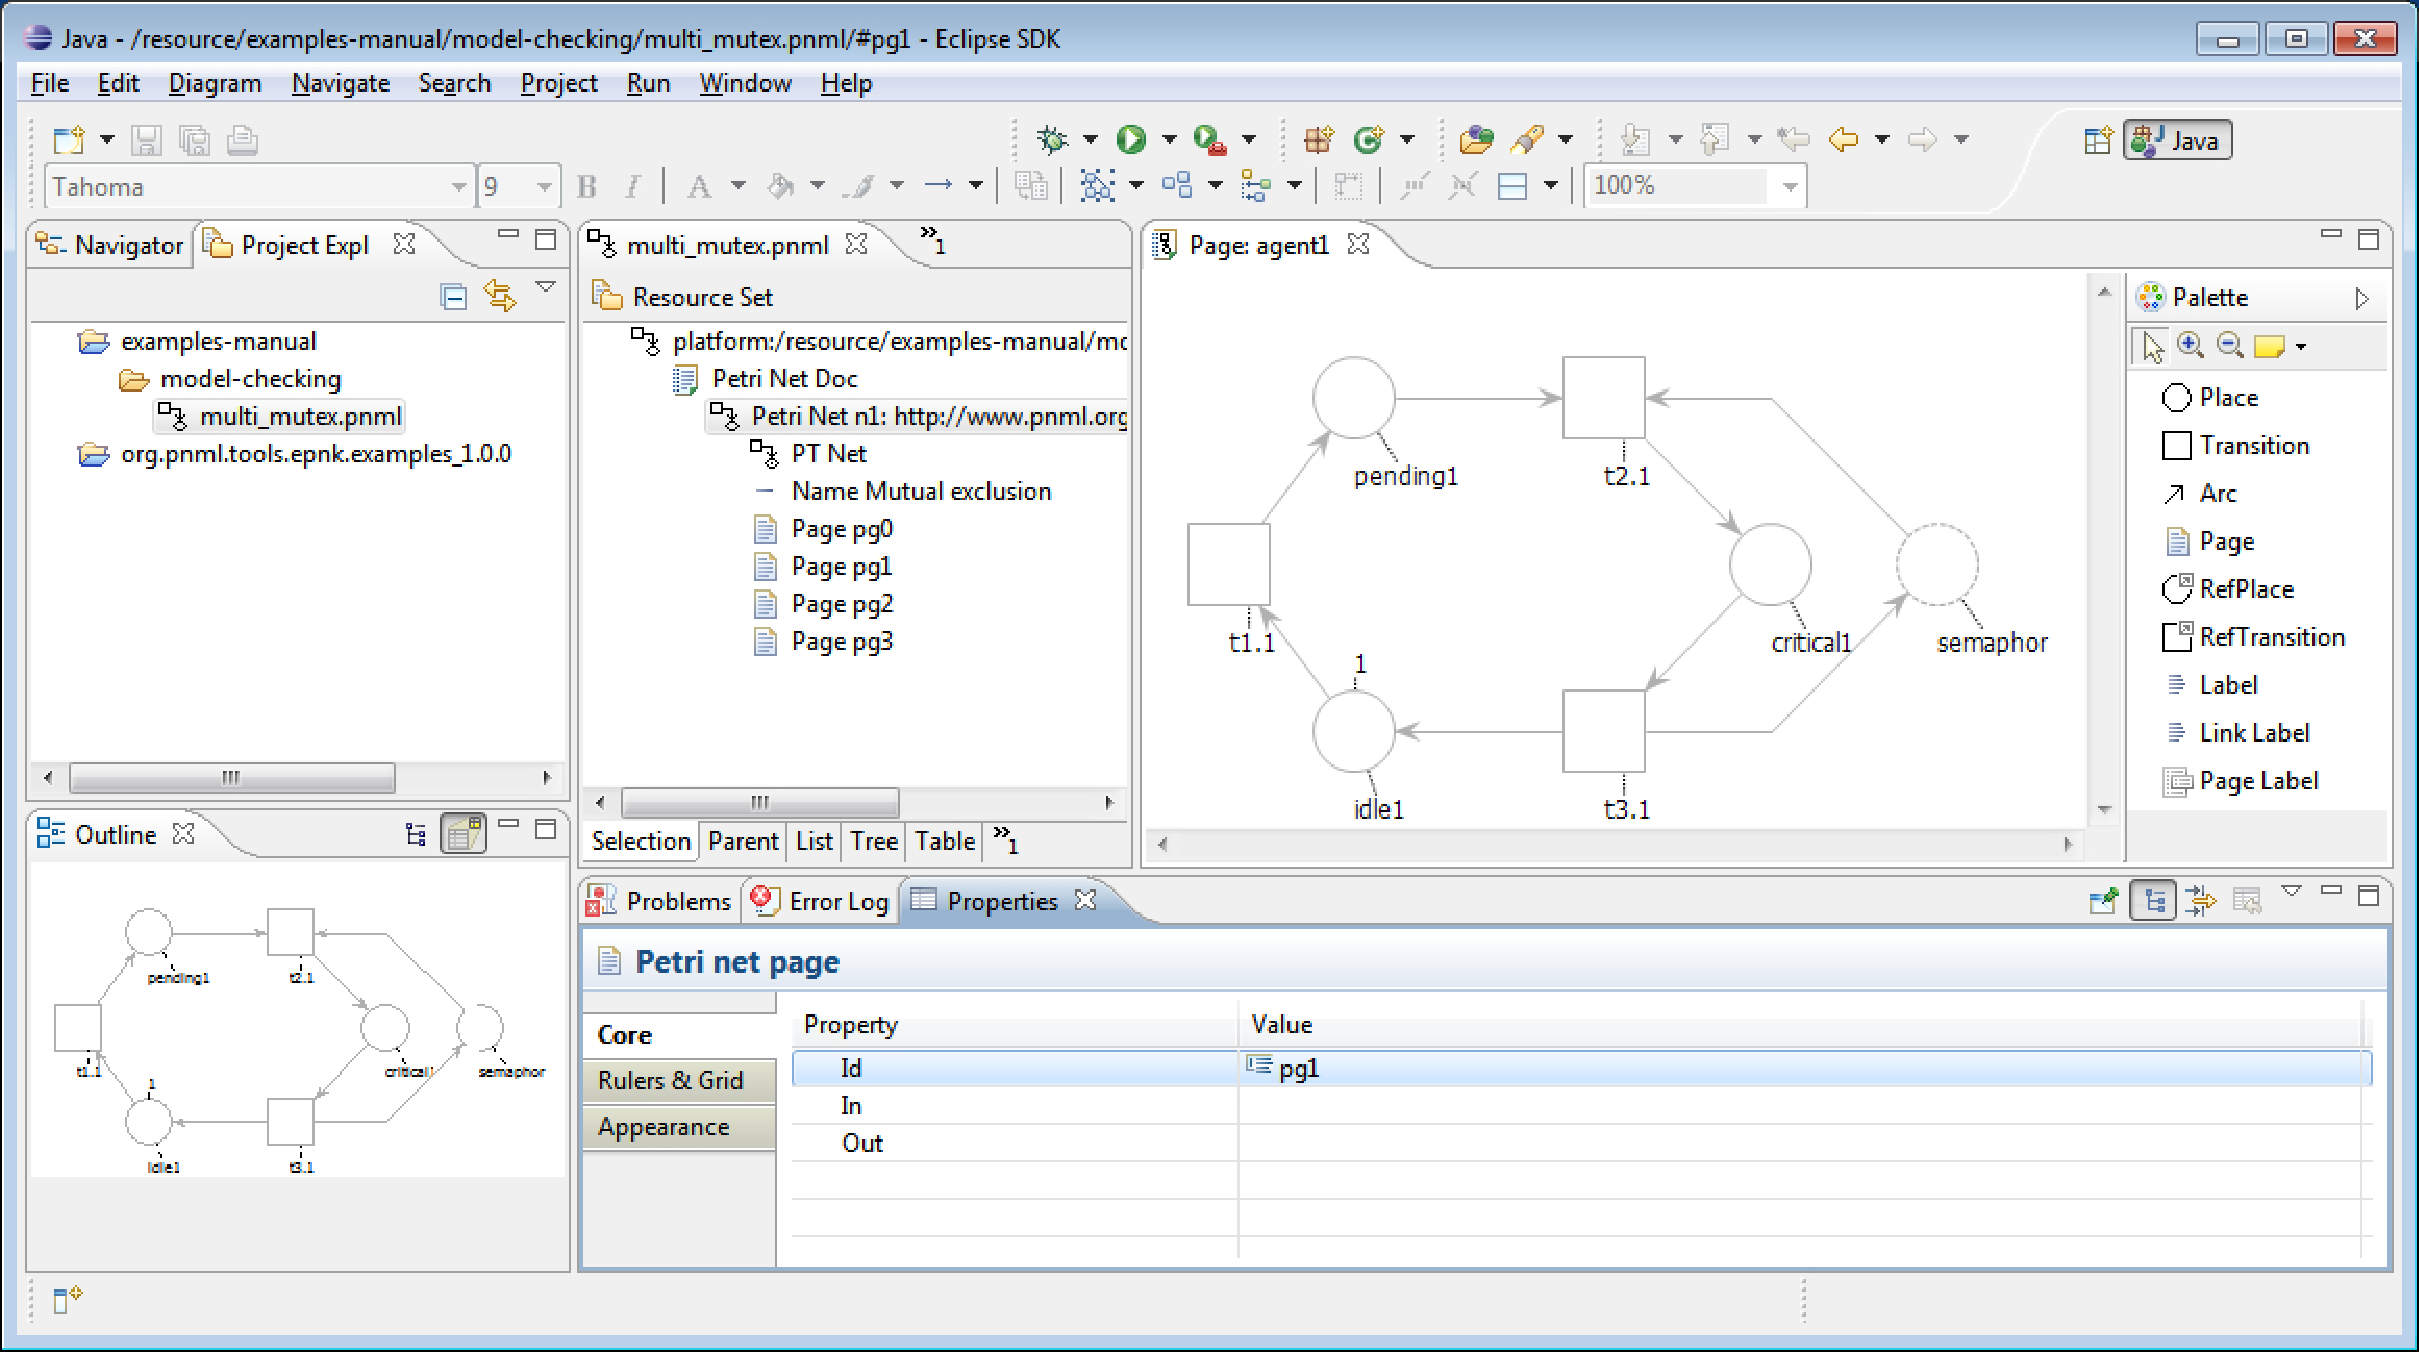
\includegraphics[scale=.30]{MultiAgents}}
  \caption{Mutex example with multiple agents}
  \label{fig:user:multi-agent}
\end{figure}
%
The three agents are competing for the semaphor in order to
access their critical section {\sf criticalx}. Actually, this
net was automatically generated by a wizard for creating a net
with any number of agents. This wizard can be initiated by
``File''$\rightarrow$``New''$\rightarrow$''Other...'' and
then selecting ``Multi-agent Mutex Net Wizard'' from the 
category ``ePNK''. 

The model checker on this net can be initiated by right-clicking
on the Petri net element in the tree editor and then selecting 
``ePNK''$\rightarrow$``Model checker''. Then, a dialog like the
one in Fig.~\ref{fig:user:modelchecker-dialog} pops up, where
two CTL formula, which make sense in any system, are provided
as a default input to the model checker:  
\begin{verbatim}
AG EX true, EG EX true # deadlock free, infinite path
\end{verbatim}
As indicated by the comments behind the hash symbols, these two
formula will check whether the system is deadlock free and whether
there is at least one infinite path.
%
\begin{figure}[hbt!!]
  \centerline{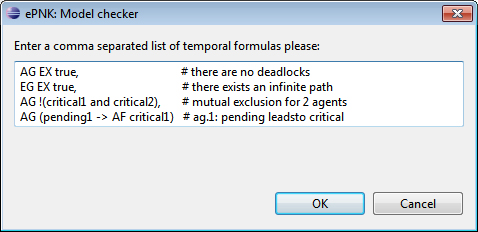
\includegraphics[scale=.40]{ModelCheckingDialog.jpg}}
  \caption{Model checking dialog: Input of formulas}
  \label{fig:user:modelchecker-dialog}
\end{figure}
%
You can of course enter some other formulas, which can use place
names in order to formulate some more specific properties like:
\begin{verbatim}
AG !(critical1 and critical2) # mutual exclusion for 2 agents
AG (pending1 -> AF critical1) # ag.1: pending leadsto critical
\end{verbatim}
For the exact syntax of the temporal formulas (CTL formulas), we refer
to the documentation of the MCiE library
\url{http://www2.cs.uni-paderborn.de/cs/kindler/Lehre/MCiE/} and its
example formulas, and we recommend to have a look into the documentation
of MCiE's parser package. Place names will be used as variables in the formula.
You need to make sure that place names of the Petri net are legal MCiE variable
names (in particular, there should not be white spaces or special characters
in them). One speciality of the syntax of CTL formulas of MCiE is that the
binary temporal operators, such as $EU$ and $AR$, are represented in infix
notation like $p1 EU p2$ instead of the more common notation $E[ p1 U p2]$.
Moreover, you can use the hash symbol \verb+#+ as a line comment --
everything following the hash symbol in the same line is ignored by the
MCiE parser. 

If the formulas entered to the dialog in
Fig.~\ref{fig:user:modelchecker-dialog} are syntactically incorrect, the
dialog will pop up again, indicating the position of the syntax error.
You can either correct the error or abort the dialog.

If the sequence of formulas is syntactically correct and the dialog was not
aborted, the model checker will be started on the net and check all the
formulas. Since model
checking can take quite some time for larger nets, the actual model checking
is done in the background, so that the Eclipse GUI is not blocked while
the model checking is done.  This is actually an Eclipse concept, which
is called \emph{jobs}. %
  \index{Eclipse!Job|DEF}
If a job should take too long, it can be aborted in the Eclipse
\emph{progress view},%
  \index{Eclipse!Progress view}
which can be easily opened while jobs are running in the background by clicking
on the \emph{progress indicator}%
  \index{Eclipse!Progress indicator}
in the bottom line to the right of the Eclipse workbench\footnote
 {If the Eclipse progress area and icon are too small for you, you can
  open the Eclipse progress view explicitly: ``Window''$\rightarrow$ ``Show
  View''$\rightarrow$ ``Other...'' and then select ``Progress'' in category
  ``General''.}.

When the model checking job is finished, this will be indicated by a
symbol in the bottom right corner of the Eclipse workbench. When you click
on it, a dialog with the model checking result will pop up. For the
net and the CTL formulas from the input dialog above, the result dialog is
shown in Fig.~\ref{fig:user:modelchecker-result}, indicating that the
first three formulas evaluate to true, the third evaluates to false\footnote
  {The reasons for this property not being true is that there are not
   fairness assumptions in this net.}.%
  \index{Model checker|)}
%
\begin{figure}[hbt!!]
  \centerline{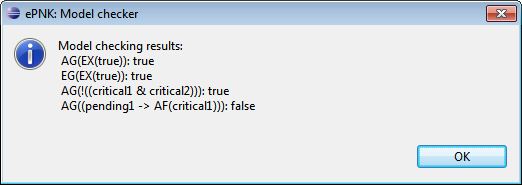
\includegraphics[scale=.40]{ModelCheckingResult.jpg}}
  \caption{Model checking dialog: Result}
  \label{fig:user:modelchecker-result}
\end{figure}


\subsection{Applications view}
\label{subsec:user:applications-view}
\index{ePNK!Application|(DEF}
\index{ePNK!Applications view|(DEF}

As mentioned above, ePNK applications are a bit more involved, since the
user can interact with them, and applications can show some visual feedback
to the user and interact with the user with visual feedback on top
of the Petri net shown in the graphical ePNK editor. One example of such
an application is an interactive simulator for high-level nets, which
is discussed in Sect.~\ref{subsec:user:hlpng-simulator}.

In order to explain the \emph{applications view}%
of the ePNK that is used for controlling the running applications and for
choosing which application the user wants to interact with, we discuss a simple
application: a simple \emph{simulator} for Place/Transition-nets.%
  \index{Simulator P/T-nets@Simulator (P/T-nets)|DEF}

Figure~\ref{fig:user:pt-sim1} shows the ePNK with a P/T-net, two of the net's
pages are open in the graphical editor. At the bottom, the \emph{applications
view} of the ePNK is shown. Note that, initially, the application view is not
open in Eclipse. You can open it in the following way: Choose
``Window''$\rightarrow$``Show View''$\rightarrow$``Other...''; then, in the opened
``Show View'' dialog select ``ePNK: Applications'' from the ``ePNK'' category.%

\begin{figure}[hbt!!]
  \centerline{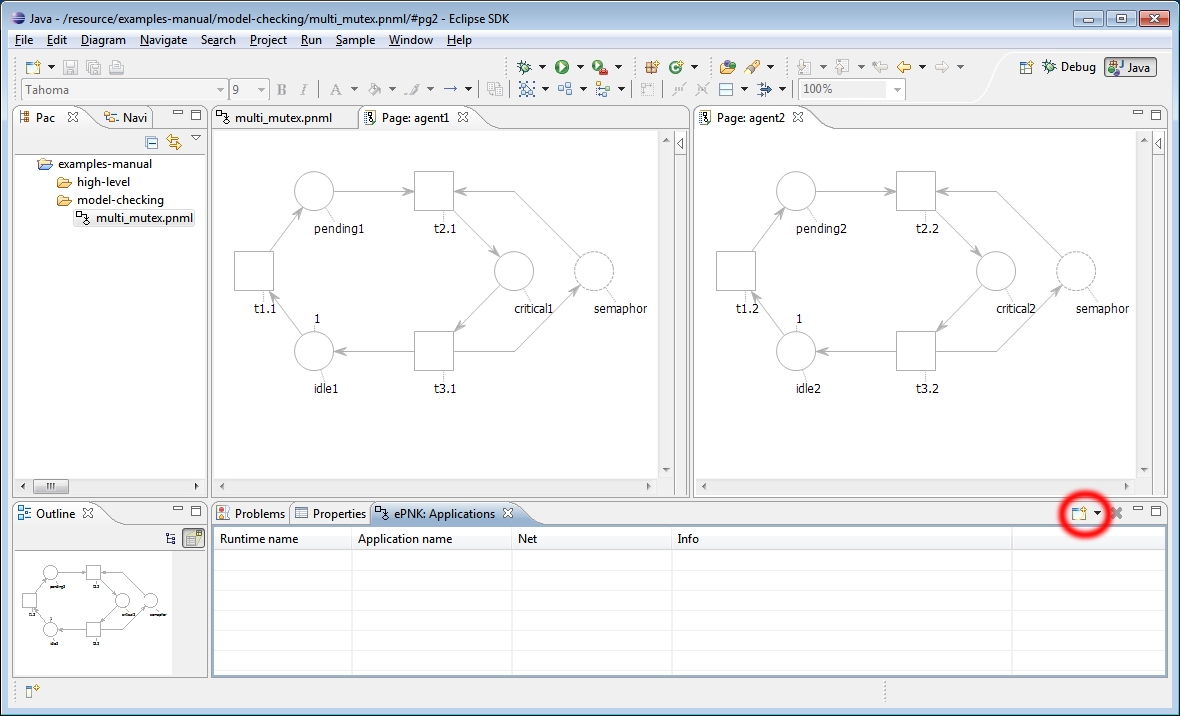
\includegraphics[scale=.30]{pt-sim1.jpg}}
  \caption{Application view a P/T-net in graphical editor}
  \label{fig:user:pt-sim1}
\end{figure}

In Fig.~\ref{fig:user:pt-sim1}, no applications are running yet. When an
editor of a net is selected, you can start an application by selecting
an application from the drop down menu, which is marked by a red circle 
in Fig.~\ref{fig:user:pt-sim1}. This menu will show all registered applications
for the selected Petri net type as well as the option to load an application
that was saved earlier, which we discuss later.

Once you have started the P/T-net simulator, the started application shows
up in the application view, and the net in the graphical editor is decorated
with some additional information. In the case of the simulator, it shows
the current marking as a blue textual label at the top-right of the respective
place; and the enabled transitions are highlighted with a blue overlay.
When the user clicks on these overlays, the respective transition fires.
Fig.~\ref{fig:user:pt-sim2} shows the simulator after the user fired
transitions {\sf t1.2} and {\sf t2.2}. Note that you might not see all graphical
feedback, since some pages are not open in the graphical editor or the graphical
editor is not on the top. You need to open the pages on which you want to see
the feedback yourself.
%
\begin{figure}[hbt!!]
  \centerline{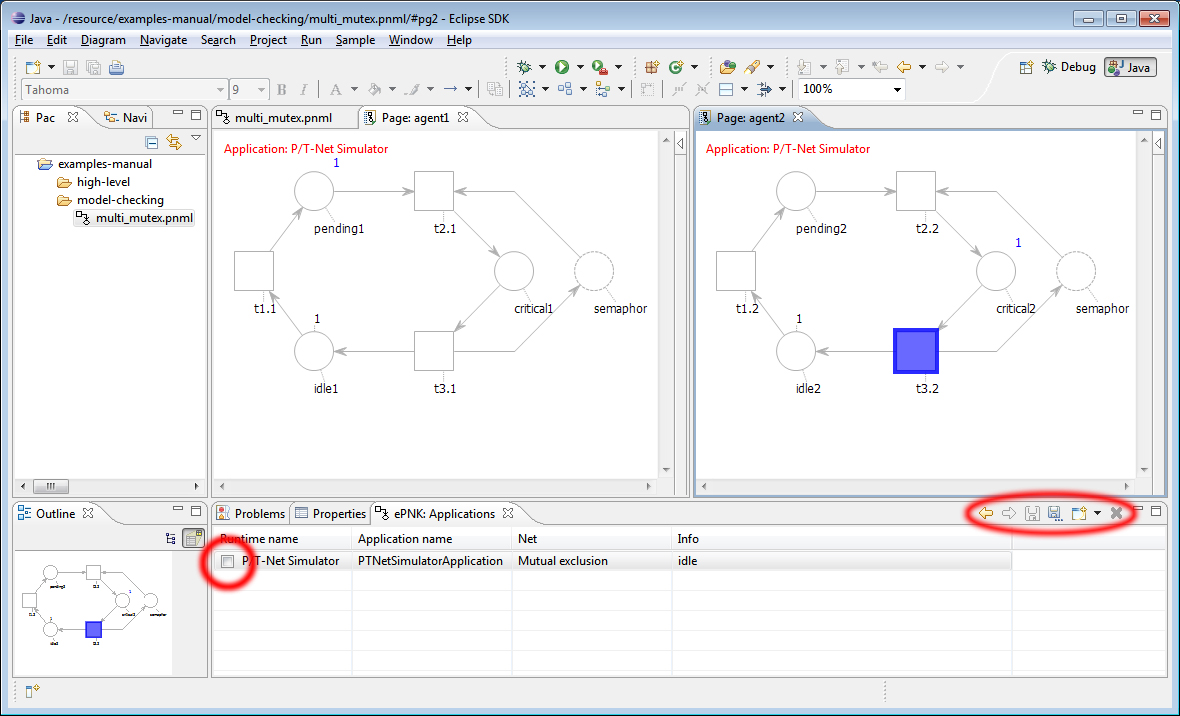
\includegraphics[scale=.30]{pt-sim2.jpg}}
  \caption{Simulator application on P/T-net running}
  \label{fig:user:pt-sim2}
\end{figure}
%
In addition, the application view
shows some more tools in its tool bar (marked in Fig.~\ref{fig:user:pt-sim2})
by a red ellipse. The back and forward buttons allow the user to navigate
to the previous or next markings, and the save buttons allow to save the
state of the simulator. The user can also start further applications by
the respective drop down menu. And the user can shut down an application
by selecting one or more applications by checking the boxes to the left of
an application, and then clicking on the delete tool. Which tools are
shown in the toolbar of the application view depends on the specific
application; but the ones shown in Fig.~\ref{fig:user:pt-sim2} are there
by default and therefore, most applications will have them.

Note that an application is always started from and associated with a net
that is open in an editor. If the editor is closed, all applications on
the respective net are shut down. But, as mentioned above, you can save
the state of an application, so that it can be restarted in that state later.
Fig.~\ref{fig:user:pt-sim3} shows the Eclipse workspace after saving the
state of a simulator by pressing the ``Save as'' button for the simulator
application. In that case the user will be prompted for a folder and file name.
The default is the same name as the net with file extension ``.apnml'' for
annotated PNML. After the first save, the state of the application can be
saved again, by simply pressing the ``Save'' button. 
%
\begin{figure}[hbt!!]
  \centerline{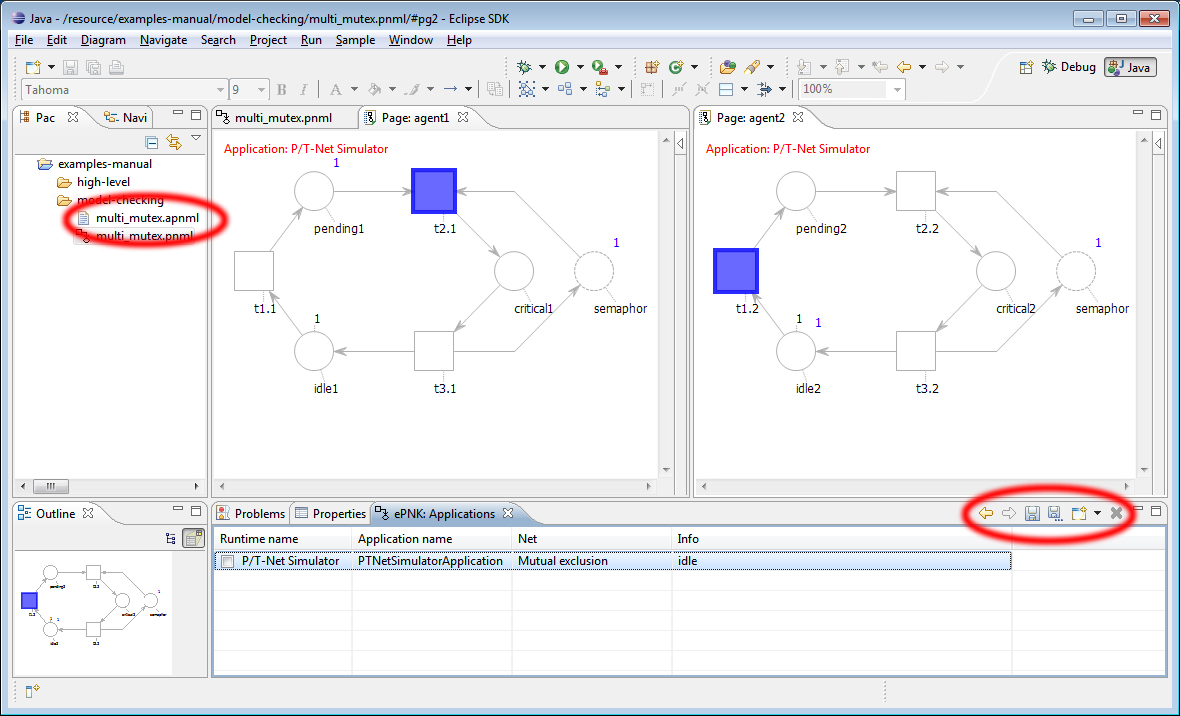
\includegraphics[scale=.30]{pt-sim3.jpg}}
  \caption{Simulator application with a saved state}
  \label{fig:user:pt-sim3}
\end{figure}
%
Later the application can be started by the drop down menu selecting
``Load application'' and then selecting the file to which the state was saved
before.

Note that there is always at most one application \emph{active}%
  \index{active application|DEF}
in the ePNK, and only the decorations of this active application are shown in
the graphical editor. But, there can be many applications running at the same time.
All running applications are shown in the applications view, and by selecting
an application there, it becomes active. You can also deselect an active
application by clicking on it with the CTRL-button pressed at the same time.%
  \index{ePNK!Applications view|)}%
  \index{ePNK!Application|)}

\subsection{A simulator for high-level nets}
\label{subsec:user:hlpng-simulator}
\index{Simulator|(DEF}

In this section, we discuss the simulator for high-level Petri nets, which is
deployed together with the ePNK. It was developed by Mindaugas Laganeckas as
part of his master's project \cite{Lag12}. The simulator is able to
simulate high-level Petri nets as well as so-called \emph{high-level net schemas}%
  \index{High-level net schema}
\cite{KiRe96,KRVW97,Rei98,HKea09,ISO-IEC:15909-2-2011}, which can
be instantiated with some communication network in order to simulate
a network algorithm on a specific network \cite{RKea98}.

Note that all examples that are discussed in this section can be obtained
from the ePNK home page together with release 1.0.0 of the ePNK:
\url{http://www2.imm.dtu.dk/~ekki/projects/ePNK/release-1.0.0.html}.

\subsubsection{The basic simulator for high-level nets}
\label{subsubsec:user:sim:basic}

We start with explaining the simulator for normal high-level nets in this
subsection and explain the simulator for net schemas later in Sect.~\ref
{subsubsec:user:sim:networks}.

Figure~\ref{fig:user:hl-simulator-1} shows the simulator application running
on a simple high-level net. The high-level net models a simple algorithm that
computes the prime numbers according to the principle of the ``Sieve of
Eratosthenes'':%
  \index{Sieve of Eratosthenes}
It starts with a multiset of all the numbers from $2$ up to some upper limit
($11$ in our example) on place {\sf numbers}. Then, the transition {\sf t}
removes a number (the value of {\sf x*y}) from this place, if this number is a
multiple of some other number (the value assigned to {\sf x}) on that place.
When no number on the place is a multiple of another number on that place, 
the transition cannot fire anymore -- and the algorithm terminates. The
numbers that are left on place {\sf numbers} are prime numbers.
%
\begin{figure}[hbt!!]
  \centerline{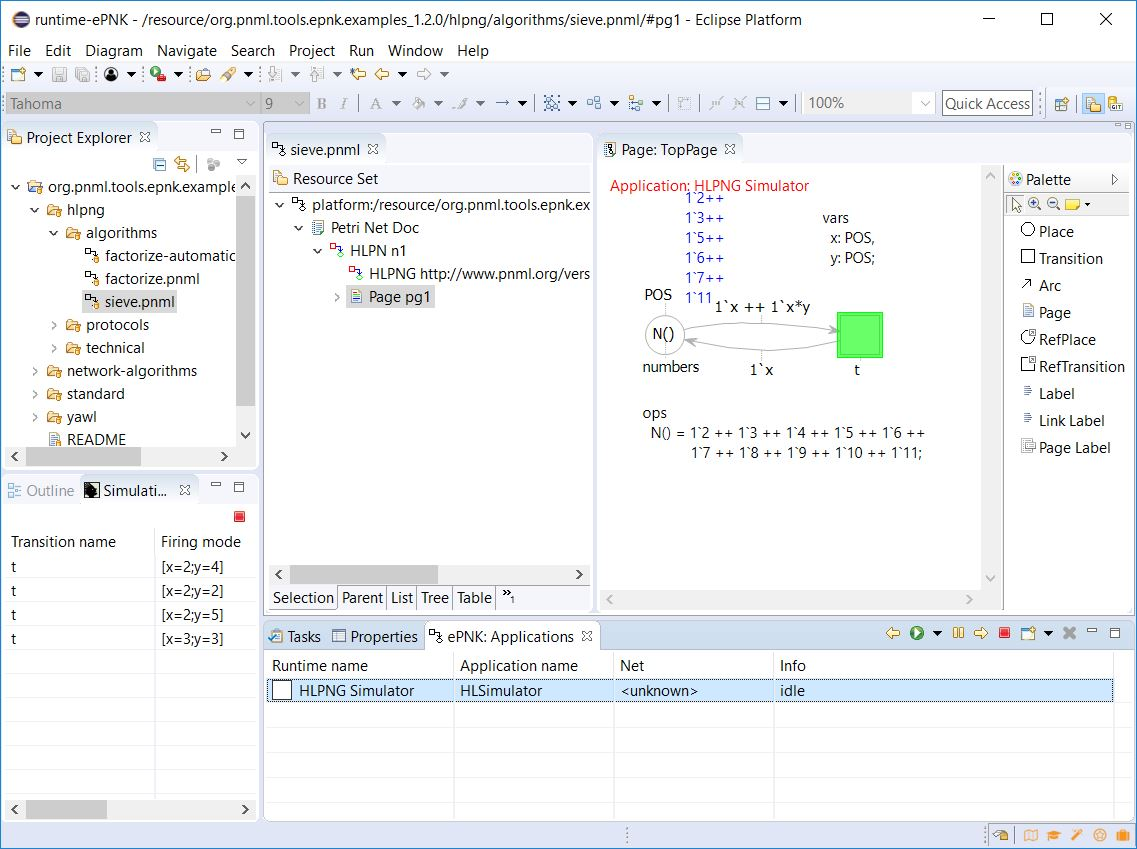
\includegraphics[scale=.33]{HL-SimulatorPrimes}}
  \caption{ePNK with a simulation application running on a HLPNG}
  \label{fig:user:hl-simulator-1}
\end{figure}
%
In Fig.~\ref{fig:user:hl-simulator-1} there is only one last non-prime
number left: $6$. The current marking of the place is shown as a blue
label at the top-right corner of the place (a long stack of tokens
represented as a multiset term in the concrete syntax for HLPNGs of the
ePNK).

Assuming that you have obtained and installed the examples from the ePNK home
page, we will now explain how to start the simulator and how to open the
additional simulator view, which shows the firing sequence up to the latest
point in the simulation. Then we will explain how to interact with the simulator.

If you did not do that yet, you need to open the \emph{ePNK applications view}%
  \index{ePNK!Applications view}
as described\footnote
  {In short:
   Choose ``Window''$\rightarrow$``Show View''$\rightarrow$``Other...'';
   then, select ``ePNK: Applications'' from the ``ePNK'' category.}
in Sect.~\ref{subsec:user:applications-view}. The \emph{Simulation view}%
  \index{Simulation view|DEF}
can be opened in a similar way: Choose
``Window''$\rightarrow$``Show View''$\rightarrow$``Other...''; then, in
the ``Show View'' dialog, select ``Simulation View'' from the ``HLPNG
Simulator Category''. By clicking on the tab at the top of the views,
you can arrange them in a way similar to Fig.~\ref{fig:user:hl-simulator-1}
-- it is convenient to see the applications view and the simulation view
at the same time.

The simulator can be started on a high-level net by right-clicking on the
HLPNG element in the ePNK tree editor and then selecting 
``ePNK''$\rightarrow$ ``Start Simulator App''.

Once the simulator application is started and selected in the applications view,
the simulation view shows the firing sequence of all transitions (along with the firing mode)
from the initial marking up to the last step of the current simulation.
If no simulation application is selected, the simulation view shows the
firing sequence of the last active simulation.  You can click on the different
entries and navigate up and down with the resp.\ buttons of the keyboard; then
the net will show the marking before the selected transition fired. The
current marking for each place is shown as a blue label at the
top right of every place -- if there is no label, the place's marking is
currently empty.

When a simulator application is selected in the applications view, you will
find several action buttons on the top right of the applications view, which
can be used to control the simulator (as shown in
Fig.~\ref{fig:user:hl-simulator-1}). The \emph{back}%
  \index{Simulator!Back button|DEF}
(left arrow) and \emph{forward}%
  \index{Simulator!Forward button|DEF}
(right arrow) buttons allow you to
navigate back and forth in the firing sequence (which had been simulated
already). The \emph{play button} (white triangle in green circle), starts the
\index{Simulator!Play button|DEF}
automatic and random firing of some transitions -- as long as there are
enabled transitions. The \emph{simulation speed}%
  \index{Simulator!Simulation speed|DEF}
can be selected by a drop
down menu on the small triangle right of the play button. It can actually
be changed while the automatic simulation is running. The automatic
simulation can be stopped -- actually ``paused'' -- by the pressing the
\emph{pause button}.%
  \index{Simulator!Pause button|DEF}
The automatic simulation can be started any time by pressing the play button
again. By pressing the \emph{stop button},%
  \index{Simulator!Stop button|DEF}
(red box), the simulator is reset to the initial marking as defined by
the net. The cross to the right will delete the simulator completely
(actually this is the general control for all applications).

The automatic simulation will randomly choose any of the currently activated
transitions, and randomly choose a firing mode. If the simulation is paused,
however, the activated transitions are high-lighted by a green overlay. You
can click on these green transitions\footnote
  {You will also be able to click on a transition which is high-lighted in grey
  or blue, as will be discussed later.}%
; then, a menu will pop up, which shows all the possible firing modes for
that transition from which you can select. Then, the transition will be
fired in the selected mode. Clicking somewhere else or pressing the ESC
button, will cancel the selection though.

Note that if you go back to some earlier state of the simulation by
selecting a transition in the simulator view or by the back button in
the simulator application, the marking at that point in the firing sequence
will be shown. You will see that one transition is high-lighted by a
blue (and darker) overlay. This is the transition to fire next in the
firing sequence as shown in the simulation view. There might also be
some other transitions high-lighted by a green overlay, which would
have been alternative choices at that point. Note that also a blue
transition might ``hide'' alternative choices that are not graphically
high-lighted, since it might be able to fire it in different firing modes.

If you are in such an intermediate state of a firing sequence, you can
still interact with the transitions by clicking on them as discussed
above and by selecting a firing mode, which will fire this alternative
transition in that marking. Note that in this case, all the later firing steps
of the earlier firing sequence are deleted.
From the current point on, a new branch of simulation will be followed.
This way, you will be able to explore different branches of the reachability
graph of the Petri net.

Note that, in some cases, the simulator is not able to compute the firing modes
fully automatically, and is not able to decide whether a transition is enabled.
In that case, the respective transition is high-lighted with a grey overlay.
This does not happen in the prime factors example, but it will happen all-over
in the example ``factorize''. Once you click on one of the transitions with a
grey overlay, you will be prompted for possible values for the different
variables. You can enter a semicolon separated list of values for each of the
variables; then the simulator will try to compute possible firing modes based on
these values.  Note that you do not need to provide values for all variables; in
many cases, it is enough to provide the value for one variable from which the
values for the other variables can be derived.  If the simulator can compute
some enabled firing modes, the transition will be high-lighted in green, so that you can
actually select the mode in which this transition should fire. You can still select
``Manual input'' for providing more or other possible values.
If no modes could be found, the transition will remain high-lighted in grey;
only if you provide values for which the transition can fire (or enough
information for the simulator to figure that out), the transition will actually
become enabled.

\subsubsection{Supported operations}
\label{subsubsec:user:sim:supported}

Note that the simulator is still in an experimental phase. In particular, some
of the more specific operations of ISO/IEC~15909-2 are not supported yet. This,
in particular, applies to the sorts and operators for symmetric nets
which currently are not supported by the simulator.

The following sorts of ISO/IEC~15909-2 are supported in the current
version (0.1.2) of the simulator: {\sf DOT}, {\sf BOOL}, {\sf NAT}, {\sf POS},
{\sf INT}, and {\sf STRING} as well as the generic sorts product, multiset
and lists over existing sorts.

The following operators are supported:
{\sf ==} and {\sf !=} on all sorts;
{\sf or} and {\sf and} on {\sf BOOL};
{\sf +}, {\sf -},  {\sf *},  {\sf /}, {\sf \%}, $<$,  and $>$ on
{\sf NAT}, {\sf POS} and {\sf INT};
{\sf concatstring} for Strings;
{\sf '}, {\sf ++}, {\sf -\,-}, {\sf all}, and {\sf empty} on multisets;
the tuple operator for products; 
{\sf emptylist}, {\sf makelist}, {\sf memberat}, {\sf sublist}, {\sf length},
{\sf appendtolist}, and {\sf concatlists} for lists.

The sorts and operators introduced for symmetric nets are not
supported by the simulator at all.
 
\subsubsection{The simulator for network algorithms}
\label{subsubsec:user:sim:networks}

In this section, we discuss the simulator for network algorithms. Before
discussing the simulator itself, we discuss the concept of network
algorithms and the way they are modelled as algebraic nets schemas
or -- in the terminology of ISO/IEC~15909 -- high-level Petri net schema
(HLPNGS).%
  \index{HLPNGS|DEF}
To this end, we use an example which -- except for syntactic sugar --
is almost identical to the first publications that used algebraic
net schemas for modelling and verifying network algorithms%
  \index{Network algorithm}
\cite{KiRe96, WWea97, Rei98}: a simple algorithm that, for a given network
of computing agents with some distinguished root agents, computes the
minimal distance of each agent from a root agent. The Petri net modelling
the algorithm is shown in Fig.~\ref{fig:user:sim:mindistance-exmpl}.%
  \index{Minimal distance algorithm}
%
\begin{figure}[hbt!!]
  \centerline{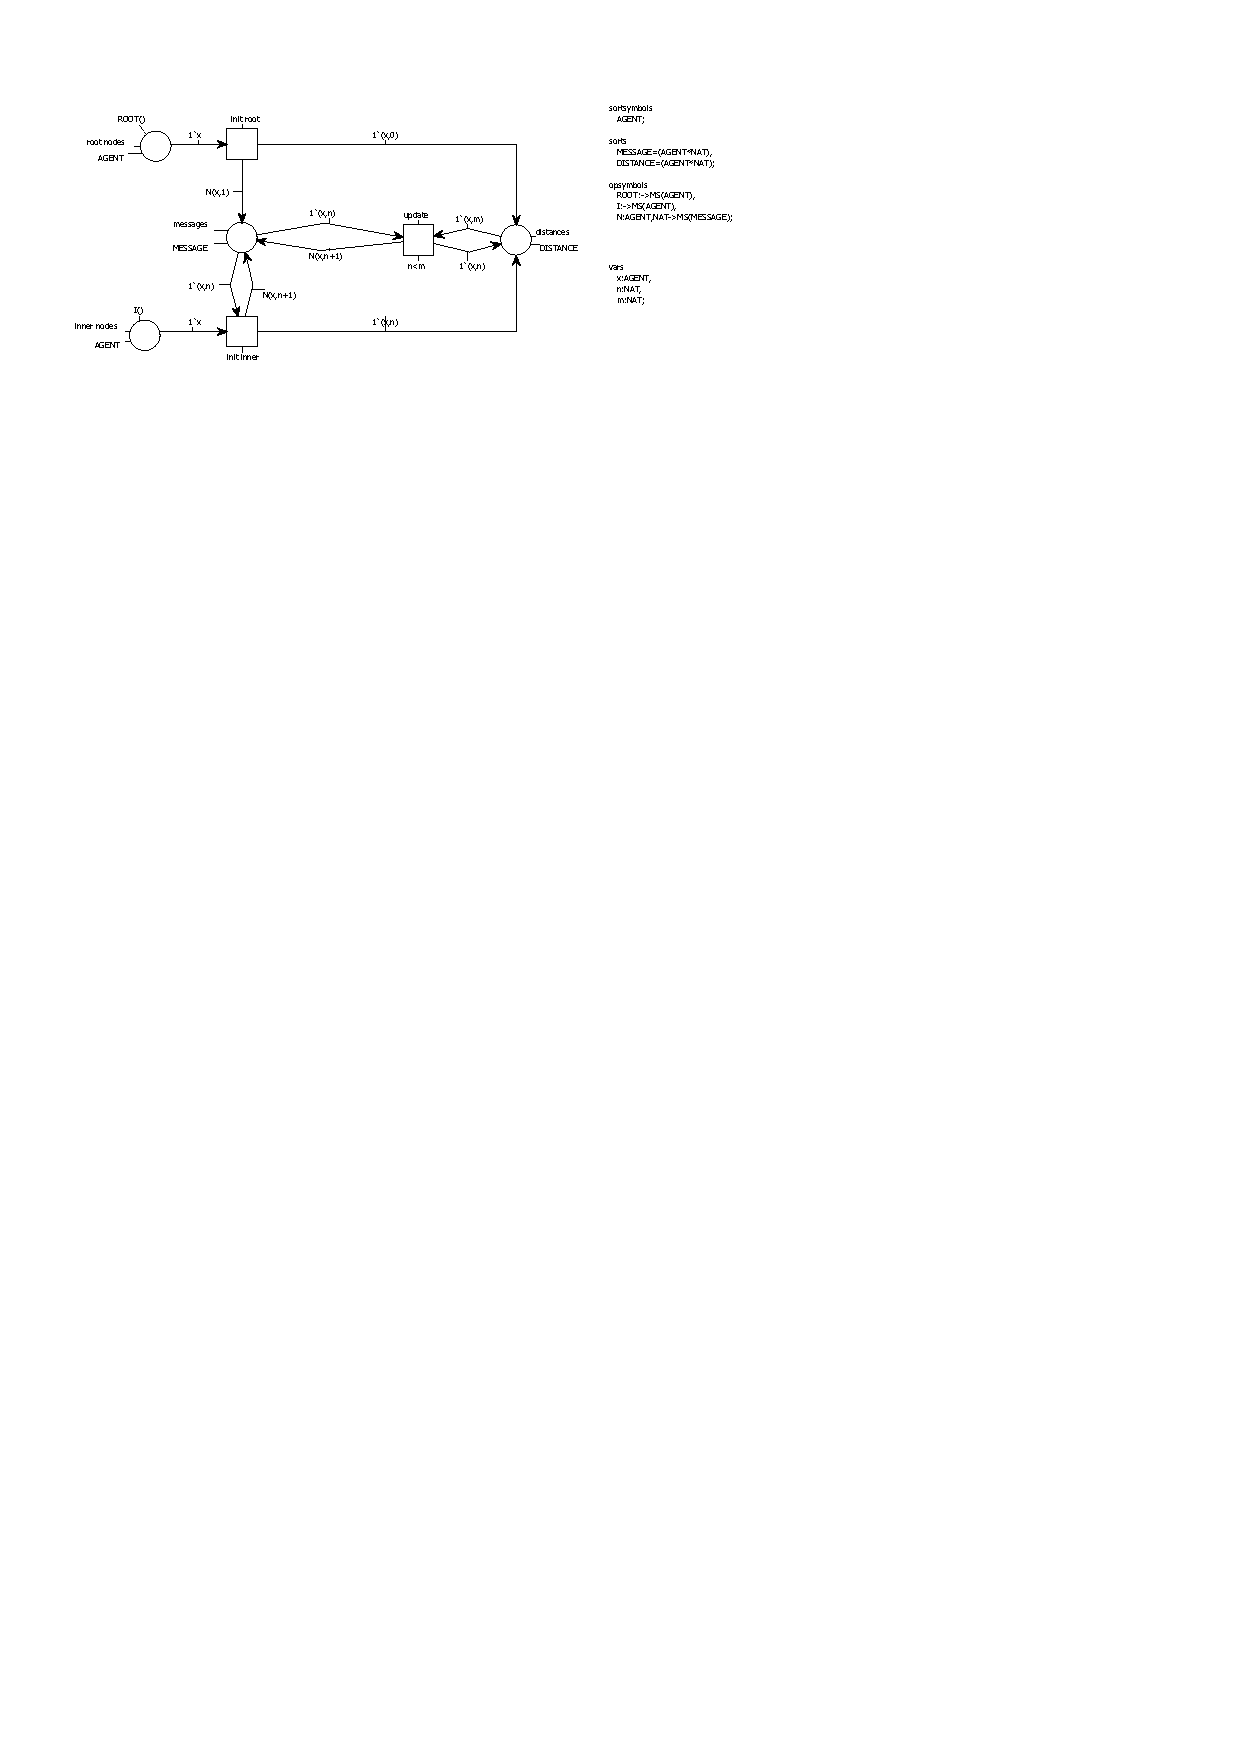
\includegraphics[scale=1.0]{MinDistance}}
  \caption{Network algorithm computing the minimal distance to a root}
  \label{fig:user:sim:mindistance-exmpl}
\end{figure}
%
In the example projects deployed for the ePNK 1.0.0, you will find it
in subfolder min-distance of folder network-algorithms.

One of the main features of a Petri net schema is that, the Petri net
model itself is completely independent from the actual network of
agents on which the algorithm is working. In the model from
Fig.~\ref{fig:user:sim:mindistance-exmpl}, the set of agents of
the network is represented by the sort {\sf AGENT}, but it is
just a symbol -- which still needs some interpretation. The
multiset constant {\sf ROOT} represents the set of root nodes,
and the constant {\sf I} represents the set of non-root nodes
(or inner nodes).

Moreover, there is an operation {\sf N}, which takes an {\sf AGENT}
and a natural number as a parameter. This function represents
sending a message from one agent to all its neighbours in the
network -- where the message itself is a natural number. A
{\sf MESSAGE} to an agent is represented by a pair, where the
first component is the receiver {\sf AGENT} and the second component
is the actual content of a message. If there is a distance computed
for some agent already, this is also represented as a pair of
an {\sf AGENT} and a number {\sf NAT} -- for making the difference
clear, we call this pair {\sf DISTANCE}.

Initially, the place {\sf root nodes} contains all the root nodes
of the network; the place {\sf inner nodes} contains all the inner
nodes. The transition {\sf init root} models the initial step of a
root node $x$: it sets its own distance to $0$, which is represented
as a pair $(x,0)$, and adds a message to all its neighbours that
they might have distance $1$ from a root node -- all these messages
are represented by $N(x,1)$. Transition {\sf init inner} models
the initial step of an inner node: when an inner node $x$
initially receives some message with some distance $n$, it stores
this distance as a potential shortest distance, and sends a
message to all its neighbours with distance $n+1$, which is
represented by $N(x,n+1)$. An inner node $x$ can later receive
other messages with another distance $n$; if the other
distance $n$ is less than its current distance $m$, the agent
takes distance $n$ as its new distance, and sends a message with
distance $n+1$ to all its neighbours. This is modelled by transition
{\sf update}.

As said before, the Petri net model from
Fig.~\ref{fig:user:sim:mindistance-exmpl} models an the minimal
distance algorithm for any network. If we want to simulate the
algorithm, we need to know on which network it should run. To this end,
a very simple network editor is deployed together with the high-level
simulator of the ePNK. Figure~\ref{fig:user:sim:network} shows the
network editor with a simple example network. In this case, it
is a network with directed arcs.
%
\begin{figure}[hbt!!]
  \centerline{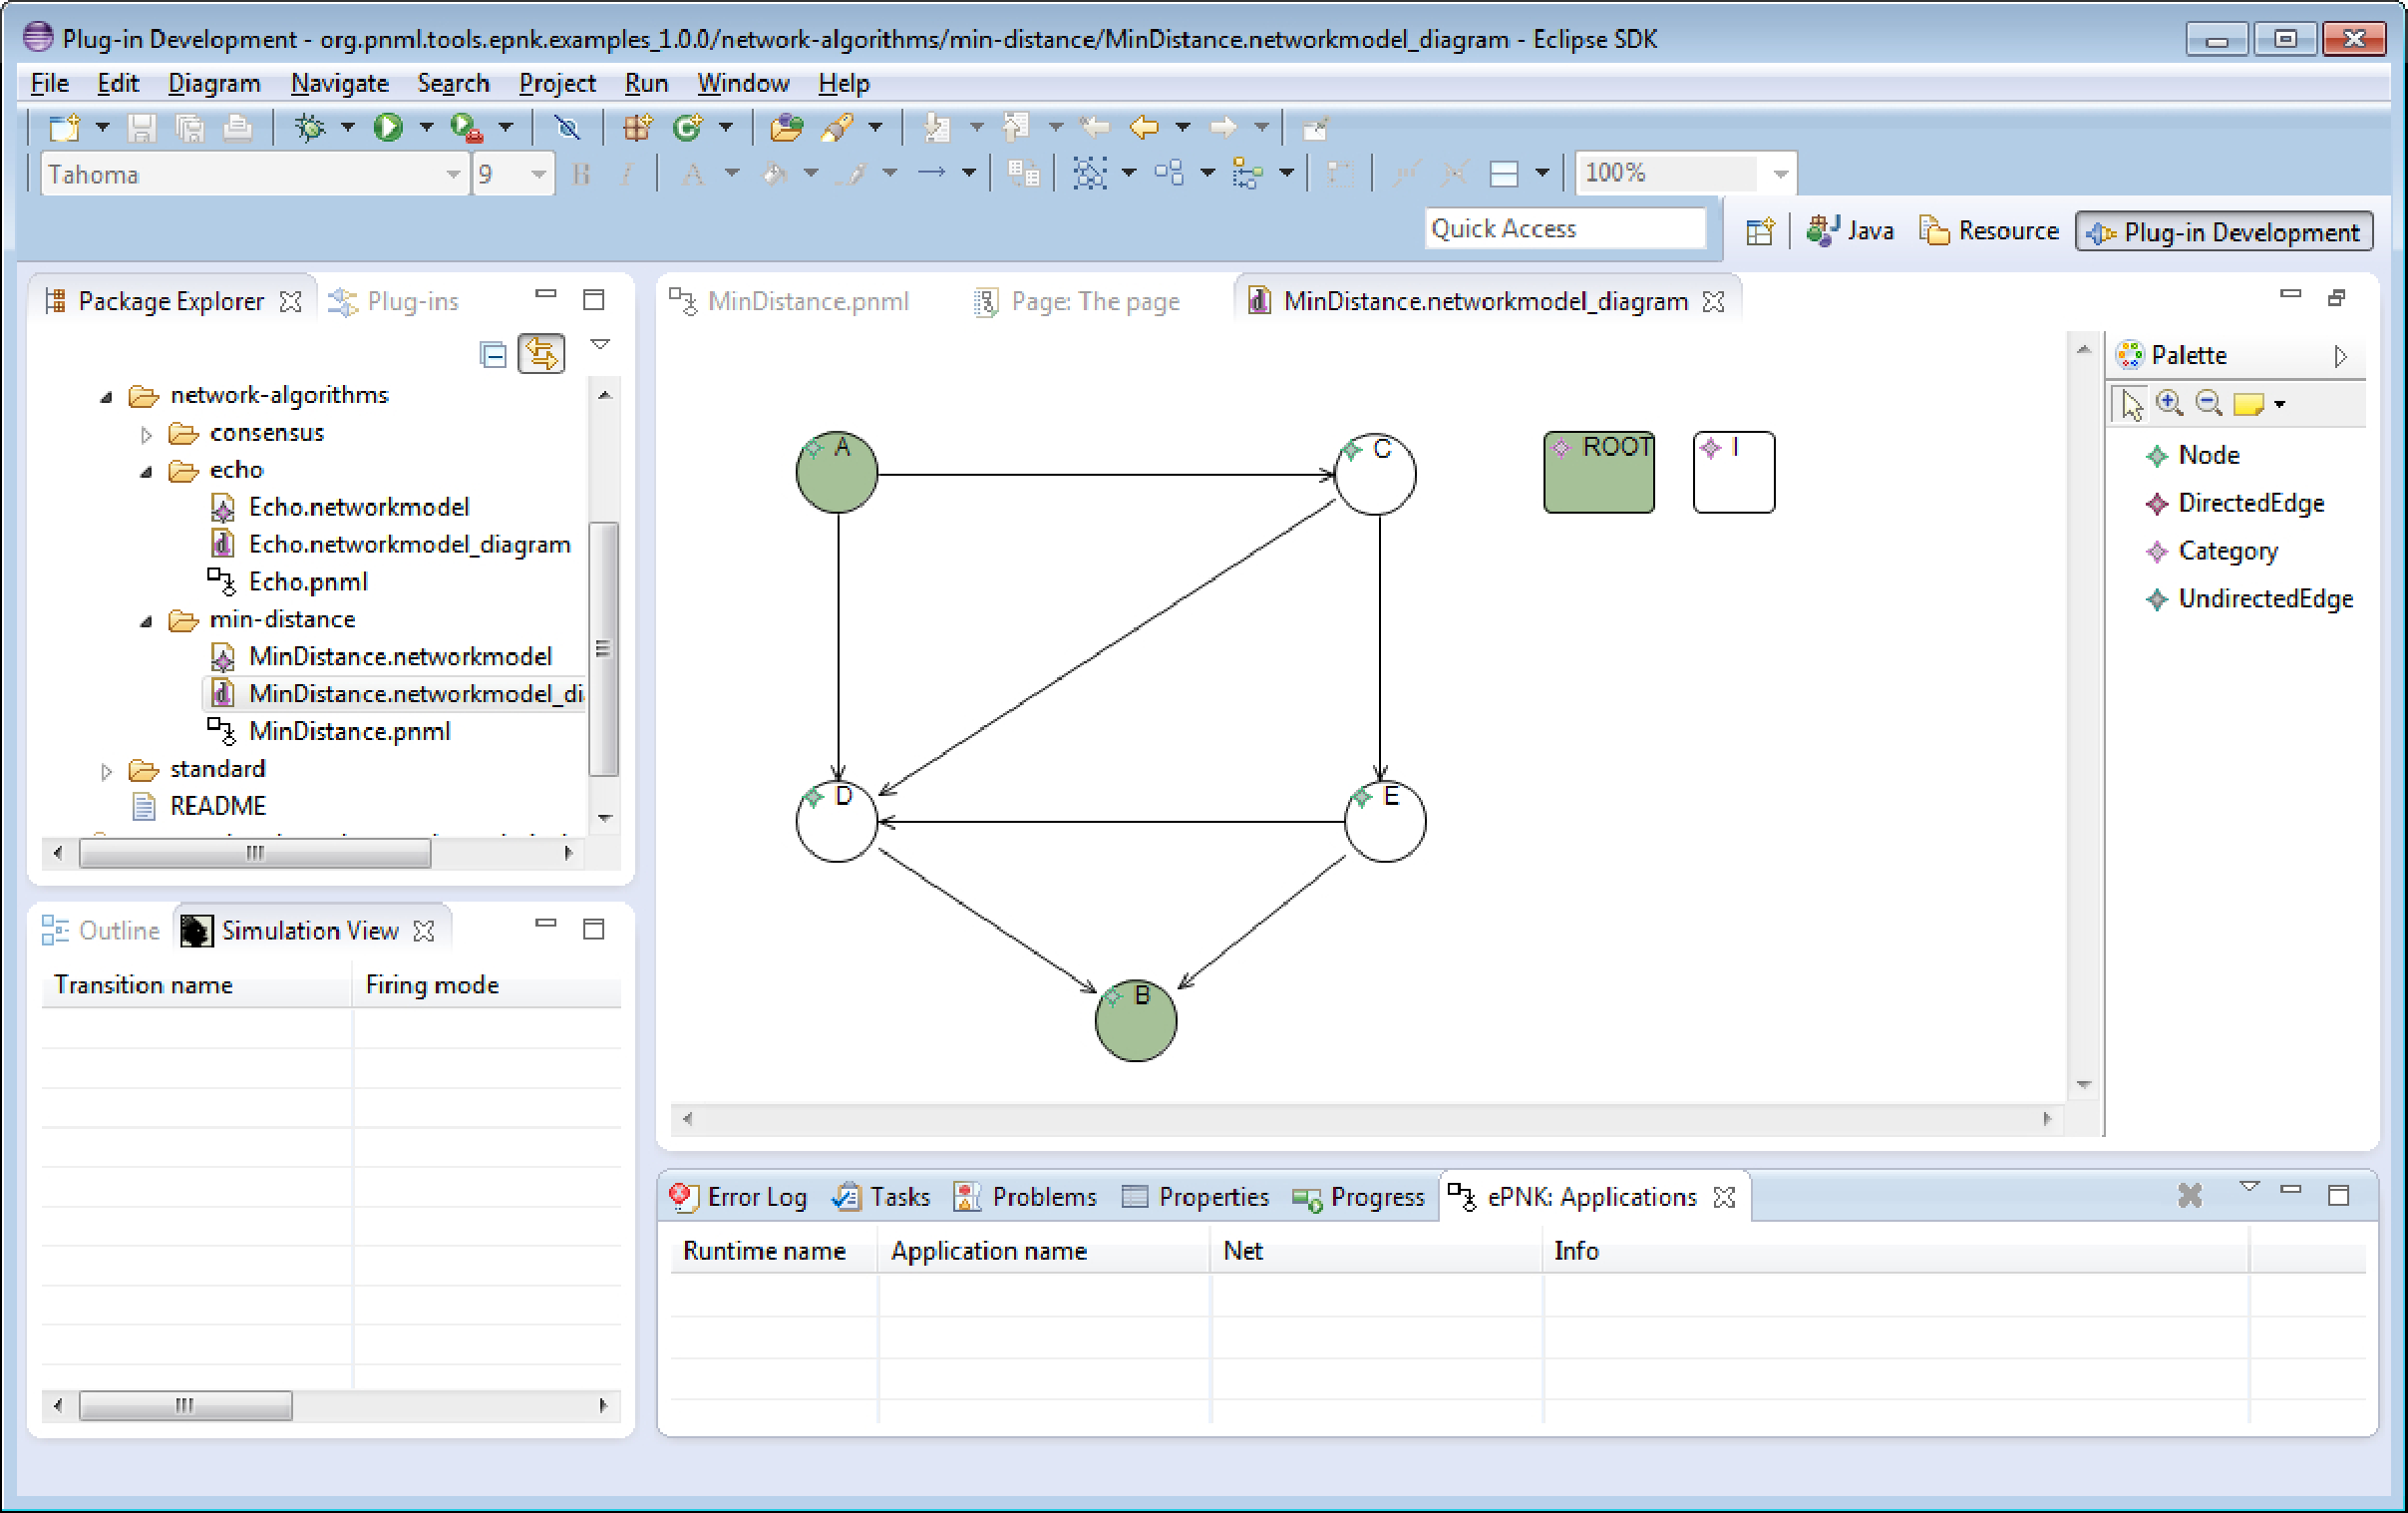
\includegraphics[scale=0.3]{Network}}
  \caption{A network on which the algorithm could work}
  \label{fig:user:sim:network}
\end{figure}
%
The network simulator can be started by right-clicking on the HLPN element in
the ePNK tree editor and then selecting ``ePNK''$\rightarrow$``Start Network
Simulator App''; if there is a network file with the same name as the Petri
net model in the same folder, the network simulator chooses this network for
the simulation. If there is no such file, the user will be prompted for
a file with a network model. Once the network model is selected, the
interpretations of the sort {\sf AGENT}, the constant symbols {\sf ROOT}
and {\sf I}, as well as the function {\sf N} (sending a message to all
the neighbours of the agent) are defined by this network. For example, for
the network of Fig.~\ref{fig:user:sim:network}, the set associated with
the sort {\sf AGENT} is $\{ A, B, C, D, E \}$; the constant {\sf ROOT}
denotes the multiset $[A, B]$, the constant {\sf I} denotes the multiset
$[ C, D, E]$; for $x = A$ and $n = 5$, the term {\sf N(x,n)} will evaluate to
the multiset $[ (C,5), (D,5) ]$ -- representing the message $5$ to each neighbor
of agent $A$. And these will be the interpretations the simulator will be using
for simulating the net.

Figure~\ref{fig:user:sim:mindistance-sim} shows the network simulator running
on the minimal distance algorithm from
Fig.~\ref{fig:user:sim:mindistance-exmpl} on the network from
Fig.~\ref{fig:user:sim:network}.
%
\begin{figure}[hbt!!]
  \centerline{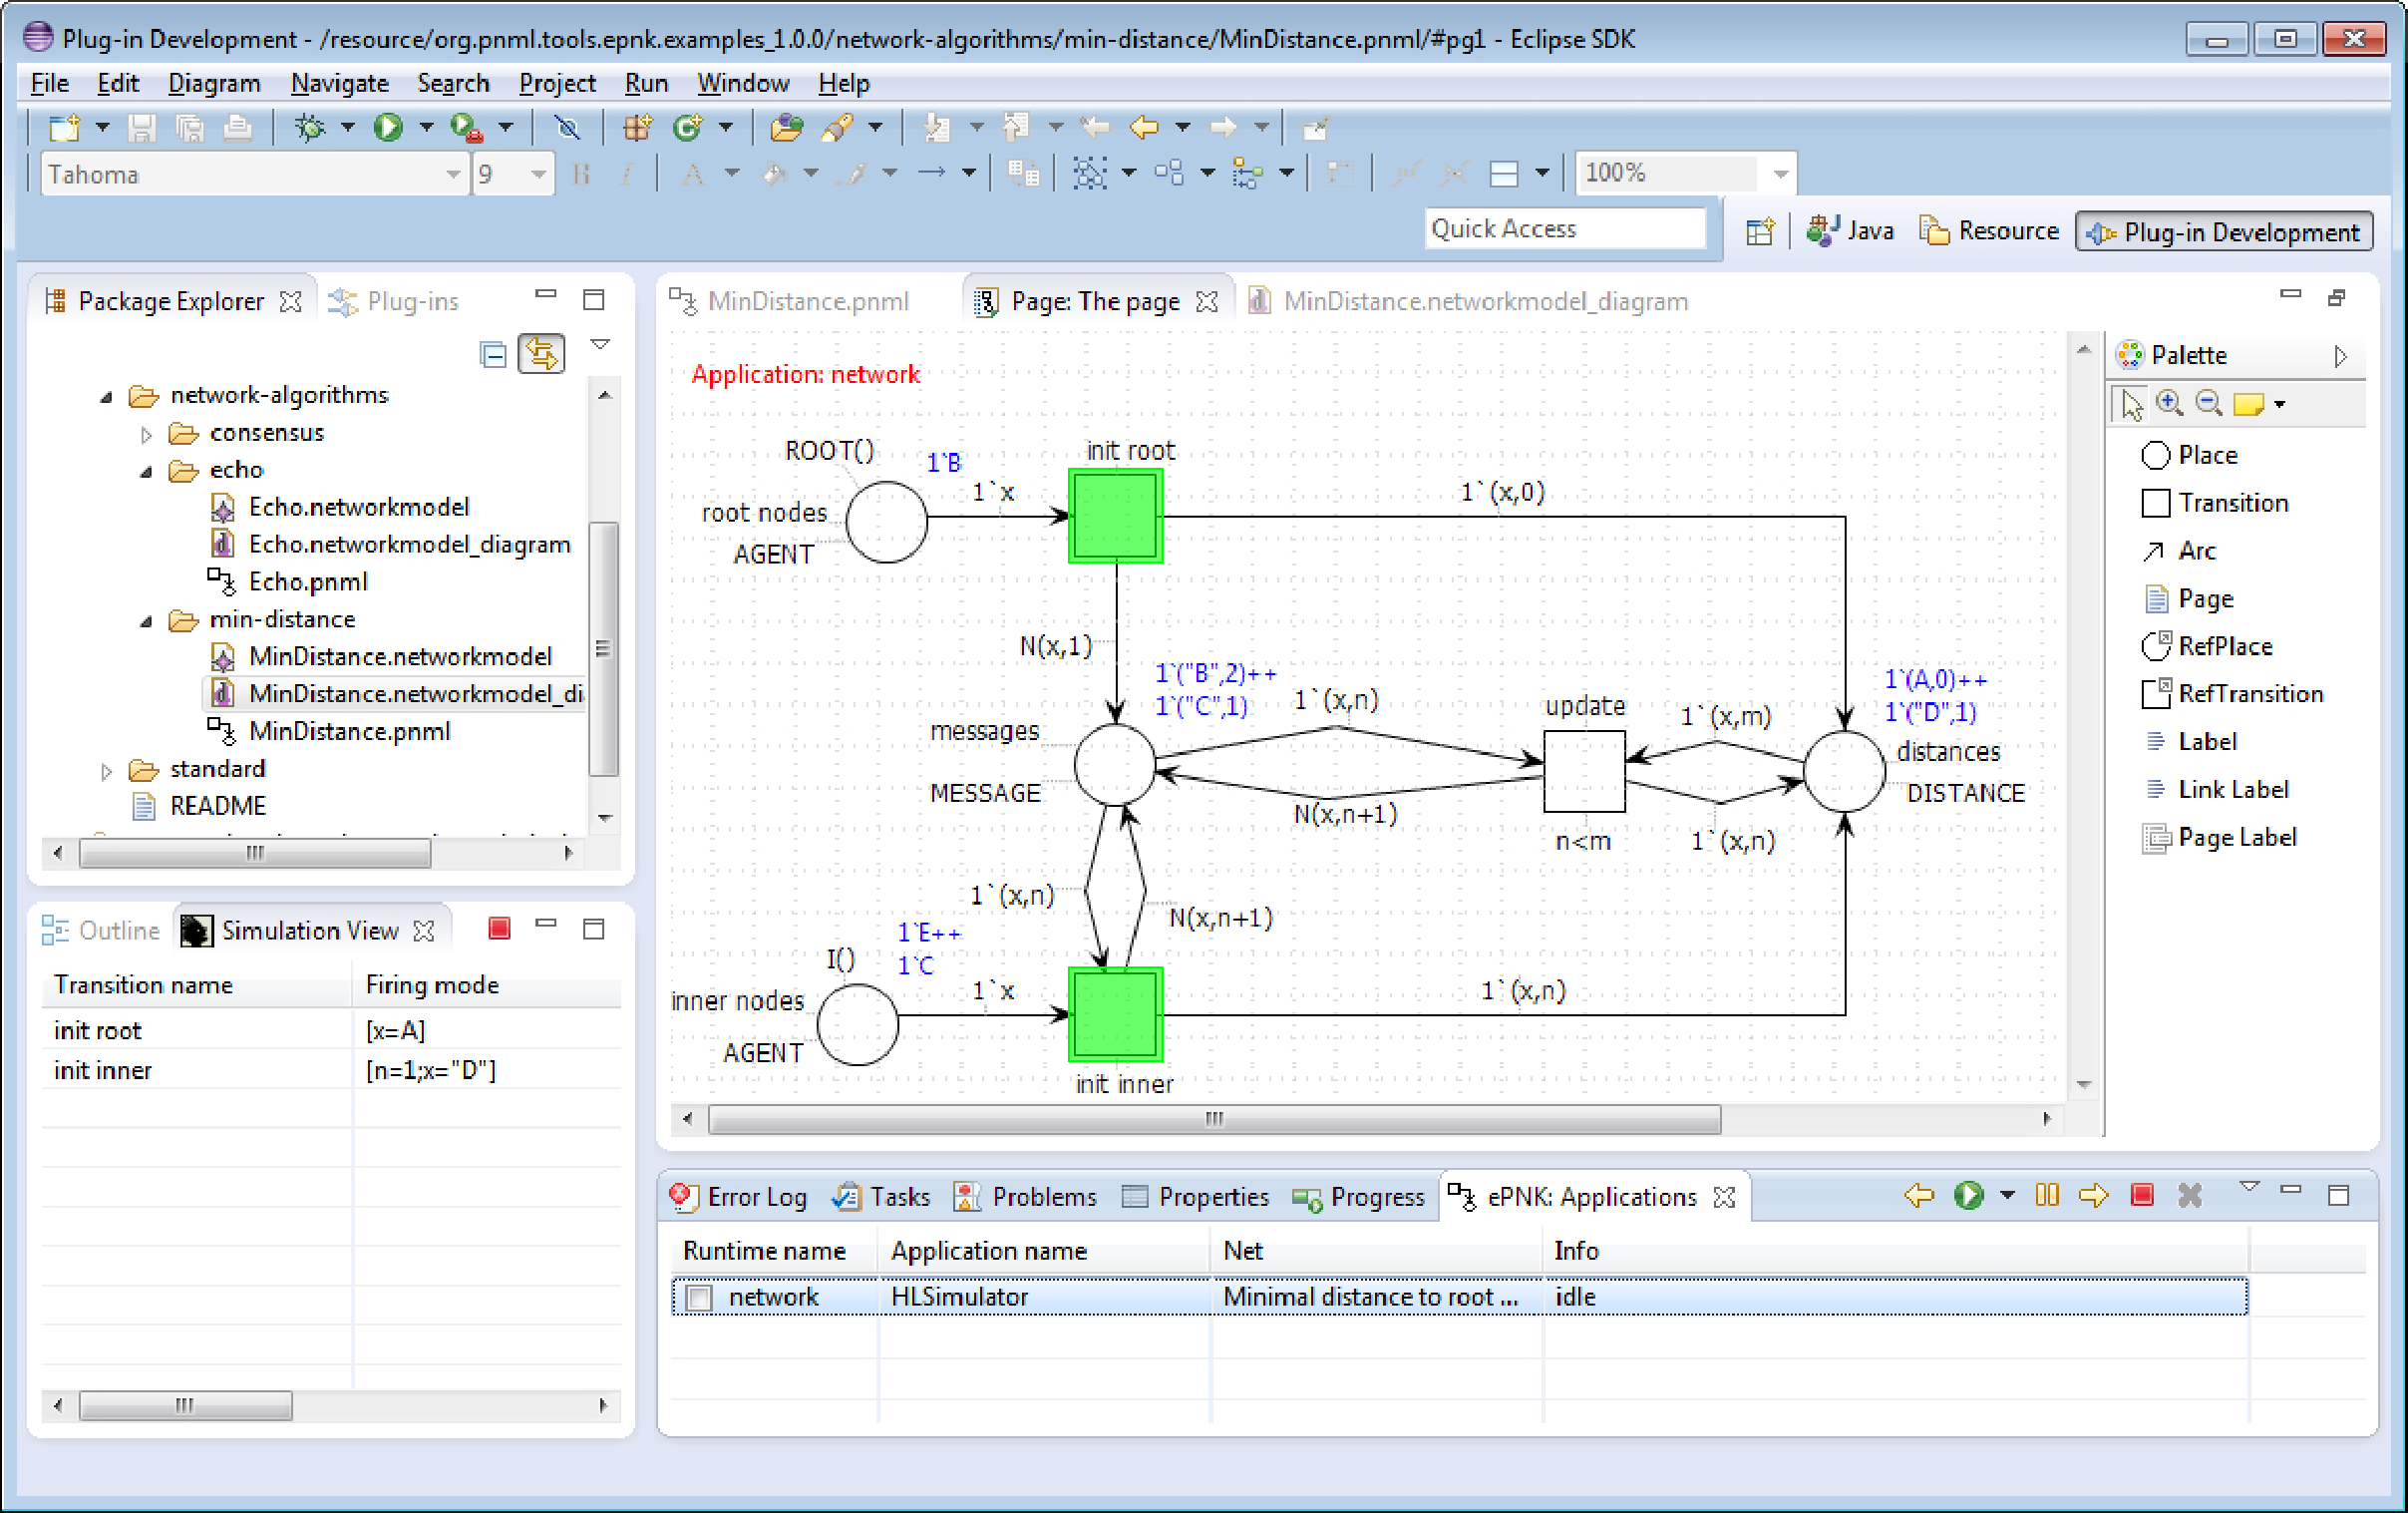
\includegraphics[scale=0.3]{MinDistanceSimulator}}
  \caption{Network simulator running on the minimal distance algorithm}
  \label{fig:user:sim:mindistance-sim}
\end{figure}
% 
The interaction with the simulator and the way to control the simulation is
exactly the same as described for the basic simulator in
Sect.~\ref{subsubsec:user:sim:basic}, once the network simulator is
properly initialized with a network.

The editor for the \emph{network}%
  \index{Network model}%
  \index{Network editor|DEF}
is a simple \emph{editor} generated by GMF
and follows the GMF philosophy. A new network can be created by
``File''$\rightarrow$ ``New''  $\rightarrow$ ``Other...'' and then
selecting ``Network Diagram'' from category ``Examples''. In this
diagram, you can add nodes, directed and undirected edges between the
nodes, as well as categories for nodes. When a node is selected,
each node can be associated with any number of categories by
a menu that pops up when clicking in the category property in
the properties view. In Fig.~\ref{fig:user:sim:network}, the
association with categories is also shown by the same colour for
the category and the resp.\ nodes; but the colour itself does not have
any meaning in the diagrams.

For a given network, the sort {\sf AGENT} is associated with
the set of nodes; for every category, the respective constant
symbol is associated with the multiset of nodes that are in
that category (in our example these are the root nodes and
the inner nodes). For the operation symbol {\sf N}, 
$N(x,m)$ denotes a multiset of pairs, where for each outgoing
arc from $x$ to $y$ there is a pair $(y,m)$ in the multiset.
$S(x)$ is a multiset of pairs over agents, where there
is a pair $(y,x)$ in the multiset if there is an undirected
arc from $x$ to $y$; these represent all messages that are
sent from agent $x$ to all its neighbours. Likewise $R(x)$ contains
all the messages received from all its neighbours. 

A Petri net modelling the echo algorithm,%
  \index{Echo algorithm}
which is another example deployed together with the ePNK, makes use of the send
and receive operations {\sf S} and {\sf R}. But, we do not explain the echo
algorithm here -- see \cite{WWea97, KRVW97} for details\footnote
  {The operation {\sf S} is denoted with $M$ and the
   operation {\sf R} is denoted with $\overline{M}$ in \cite{KRVW97} -- and
   the other way round in \cite{WWea97}.}%
.%
  \index{Simulator|)}

\section{Limitations and pitfalls}  

The current version of the ePNK (1.0.0) still has some minor limitations,
which are discussed in this section in order to avoid some unpleasant
surprises. If you identify other issues or problems, please, let us know. 
  
\subsection{Saving files: Tree editor}
Technically, the tree editor and the graphical editor for pages are
different editors. The graphical editors can be initiated via
the tree editor only (via the pop-up menu ``Start GMF Editor on Page'' or
a double click on a page in the tree editor or the graphical editor).
The tree editor, however, serves as the main editor; saving a PNML document
is possible only from the tree editor -- and only the tree editor
shows a valid ``dirty-flag'' when the file contains unsaved changes
(see Sect.~\ref{subsec:save-documents})

\subsection{Reset an attribute}
\label{subsec:user:reset-attribute}
In case some attribute is set to some value and you would like to remove
that value (meaning that actually, the attribute is removed completely),
it is no good to enter an empty string as a value for that property. And
if it is an attribute with finitely many possible values, the drop down
menu does not give you an option to not select any value. To restore
the default situation of unsetting the attribute, you can right-click
into the property column of that attribute in the properties view and then
select ``Restore default value'' (see Sect.~\ref{subsec:attributes}).


\subsection{Graphical features}
\label{subsec:supported-graphical-features}

The graphical editor of the ePNK supports many graphical features, such as
positions and size of nodes, intermediate positions for arcs, fonts, size and
colours for labels, colours and line-width for nodes and arcs. Up to now, not
all of these graphical features are transferred back to the actual
PNML document (some of this information it is not even supported by PNML).
Some graphical information is stored only as (ePNK) tool specific information.

The graphical information that is used and made available in PNML
so that it can be used by other tools that support PNML is the following:
\begin{itemize}
  \item Position and size of nodes.
  \item Line colour and background colour for nodes.
  \item Image information for nodes\footnote
          {Up to version 1.0.0 of the ePNK, the path to an image can be changed
          only in the tree editor. But the image is shown in the graphical editor
          once it is set. From version 1.0.1 and higher, it will be possible to
          set the image URI in the properties view of the node directly}.
  \item Position resp.\ relative position of labels\footnote
          {The size of labels is not supported by PNML}.
  \item Text colour\footnote
          {For the text colour the ePNK is actually abusing the line colour
           attribute of PNML, since PNML does not have a text colour
           attribute.}
        and background colour for labels.
  \item The font and the font-size of labels.
  \item Intermediate points of arcs.
  \item Line colour of arcs.
  \item The shape attribute of arcs (straight or bezier).
\end{itemize}

Note that all the graphical information -- even the one that is not transferred
to PNML features -- is saved by the ePNK as tool specific information. You can
even put notes on the graphical canvas, which will be saved. The graphical
information not covered in the above list, however, will not be available to
other tools, and will be gone, when the tool specific information
(org.pnml.tools.epnk.diagraminfo) for the resp.\ page is deleted.

The ePNK reads all graphical attributes that are supported by PNML;
but, only the ones discussed above are used and shown in the graphical editor.
Moreover, the unused graphically attributes are not checked for
validity; they will be written exactly the same way they were, when
loading the PNML file (see also Sect.~\ref{subsec:graceful-PNML}).

Due to some limitations in the automatically generated GMF editor on which
the graphical editor of the ePNK for pages is based, there is another quirk
of the graphical ePNK editor: When a node is moved, the intermediate points of
the attached arcs are also changing in the diagram; these changes are, however,
not propagated to the PNML model. If you want to make sure that the
intermediate points of an arc of the diagram and the PNML are exactly the same,
the you need to explicitly touch and slightly move an intermediate point of each
attached arc -- only then, the exact positions of the intermediate points
are properly propagated to the PNML model.

Note that some Petri net type definitions might define some graphical appearance
for some of its elements. In that case, this graphical appearance overrides the
graphical attributes of PNML.

\subsection{Petri net types}

As mentioned in Sect.~\ref{subsec:creating-elements}, the type of a Petri net
should never be changed after a net of that type was created --
unless you know exactly what you are doing. Otherwise, it could happen
that the produced PNML is invalid.

For HLPNGs, it is no problem to change its kind any time, since this
kind has an effect on the validation only, but no effect on the
serialisation of the net to a PNML file. Changing the ``kind'', actually,
does not change the Petri net type -- just the sub sets of features that
are supported.

 
\subsection{Wrapping labels}

All labels in ePNK can have line-breaks. In the graphical editor,
line-breaks can be added by pressing the CNTRL and ENTER at the same time.

\subsection{Graceful PNML interpretation}  
\label{subsec:graceful-PNML}

PNML files that are produced by the ePNK and which have been successfully
validated are conformant to PNML as defined in ISO/IEC~15909-2. The
only exception is, when some illegal graphical attributes are read from an
existing PNML file; these attributes will not be touched by the ePNK, and
therefore written again -- even if they are not conformant to ISO/IEC~15909-2.
But, if a PNML file is created by using the ePNK only and if it validates
correctly, the saved file is PNML conformant.

The ePNK, however, is not a PNML validator. It reads PNML and ``PNML-like''
documents and writes them again in a graceful manner. This way, it is possible
to save PNML documents that do not properly validate; and the ePNK is able to
load these files again even though other PNML tools might not be able to
load them. For example, when some elements do not have ids (as required
by PNML), references to these elements cannot be made via their id. In that
case, the ePNK uses XPath references to these elements, which is not conformant
to PNML. If such an invalid PNML file is loaded later by the ePNK again,
the ids are added then, and validation is successful, saving this
file  will produce a conformant PNML documents again.

\subsection{Deviation from PNML}
\label{subsec:user-netlabels}

There is one minor deviation of the ePNK from PNML as of ISO/IEC~15909-2:2011:
In the ePNK, all declarations of HLPNGs can have a name attribute, 
which comes from the fact that {\tt Declaration} implements the interface for
symbol definitions ({\tt SymbolDef}). As a consequence, also the {\tt Unparsed}
declaration can have a name attribute. In ISO/IEC~15909-2, {\tt Unparsed} does
not have a name attribute -- as the only exception among all declarations of
PNML. Therefore, if an {\tt Unparsed} operation declaration with a name
attribute would be manually added to a PNML document in the ePNK tree editor,
the resulting PNML document would not be conformant to  ISO/IEC~15909-2:2011 anymore.

In practice, however, this should not be any problems, since the only
way to add an unparsed declaration to a HLPNG net would be to add it manually
via the ePNK tree editor. If all declarations are edited in the graphical
editor by editing the respective labels, this problem will never arise.
If the PNML document would contain an {\tt Unparsed} operation declaration
without a name attribute (as it would be according to the standard), the
ePNK would show this as an error under validation. But, it would still be able
to read and write the PNML document.

In future versions of ISO/IEC~15909-2\footnote
  {Currently ISO/IEC~15909-2:2011 is under revision, which might fix
   this problem in the standard.}, this might be resolved by requiring that
all declarations -- including {\tt Unparsed} -- should or, at least, could have
a name attribute.
